\subsection{\tty production Measurement in SLDL phase space:}
\label{sec:tty_prod_sldl_measurement}

In this section, we will present results of the unfolded likelihood fit using data for the \tty production cross section measurement in SLDL phase space mentioned in Section ~\ref{sec:fiducial-phase-space}. After the fit, the resulting post-fit $p_T(\gamma)$ distribution are shown in Figure~\ref{fig:pt_postfit_sldl_realdata}. The resulting pulls of the NPs  are shown in Figure ~\ref{fig:pull_plot_pt_sldl_mu_blinded_tty_prod}, and the correlations in Figure ~\ref{fig:NP-corr_sldl_mu_blinded_tty_prod} and Figure ~\ref{fig:NP-corr_sldl_mu_blinded_tty_prod}. The post-fit value of all the NPs changed within 1 $\sigma$, with a large fraction of the NPs having very small pulls and constrains, which indicate that the fit is robust and not affected by any unexpected behavior of the NPs. Ranking plots are shown in Figures ~\ref{fig:ranking_sldl_tty_prod_mu_blinded} . The unfolded distributions at particle level are shown in Figure ~\ref{fig:pt_unfolded_dist_sldl_tty_prod_realdata}. Furthermore the normalised unfolded distributions are shown in Figures ~\ref{fig:tty_prod_diff_SLDL_norm}. The decomposed uncertainties of the unfolded distributions for the absolute and normalized differential cross-sections are illustrated in Figures ~\ref{fig:tty_prod_diff_SLDL_groupedimpact} and ~\ref{fig:tty_prod_diff_SLDL_groupedimpact_normalized}.   $\chi^2$/ndf and $p$-values between the measured absolute and normalised cross-sections of \tty production and the NLO \MGNLO simulations interfaced with \PYTHIA[8] and \HERWIG[7] are shown in Table ~\ref{tab:chi2_ttyprod_sldl}.


\begin{figure}[ht]
  \centering
  \subfloat[]{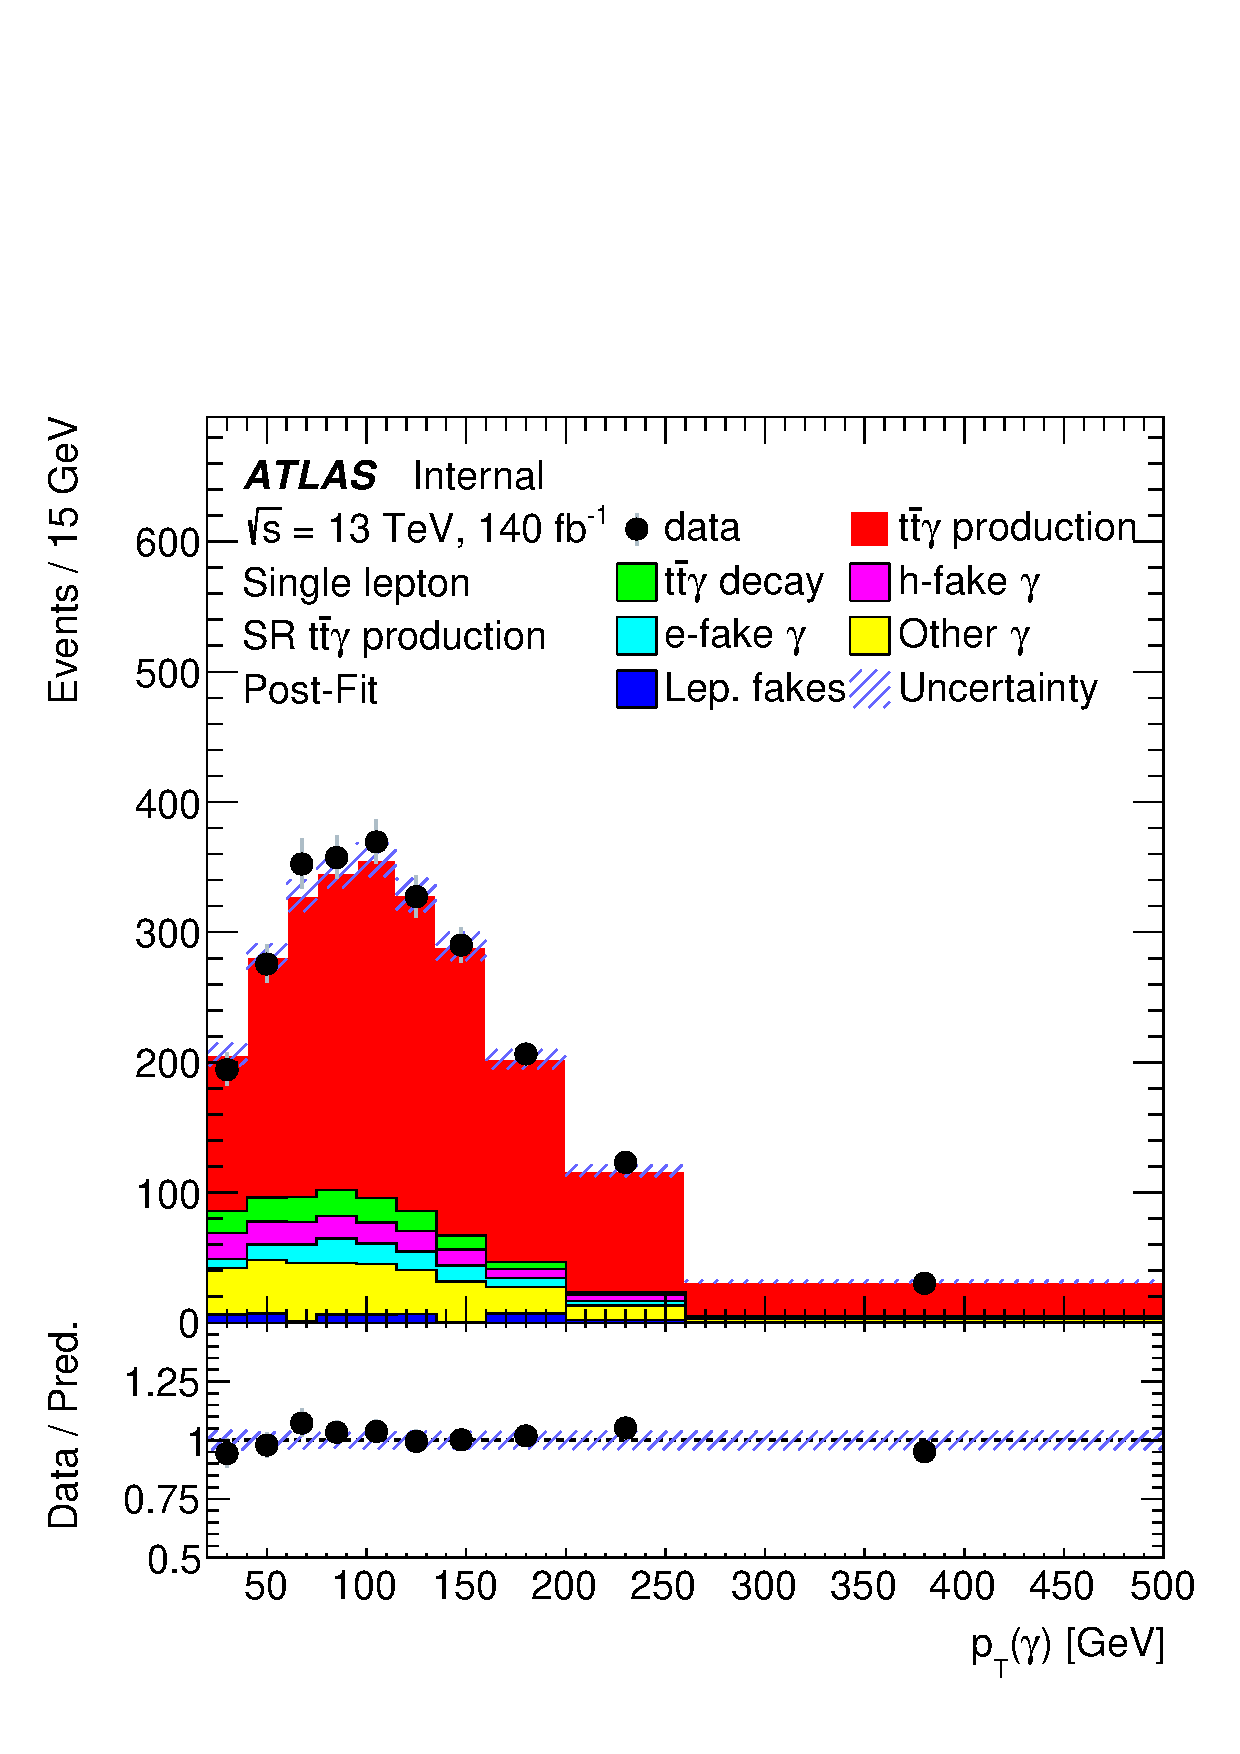
\includegraphics[width=0.30\textwidth]{figures/diff_xsec/ljet_dilep_combination_mu_blinded/post-fit/tty1l_pt_all_syst/SR1_ljet_postFit.pdf}}
  \quad\quad
  \subfloat[]{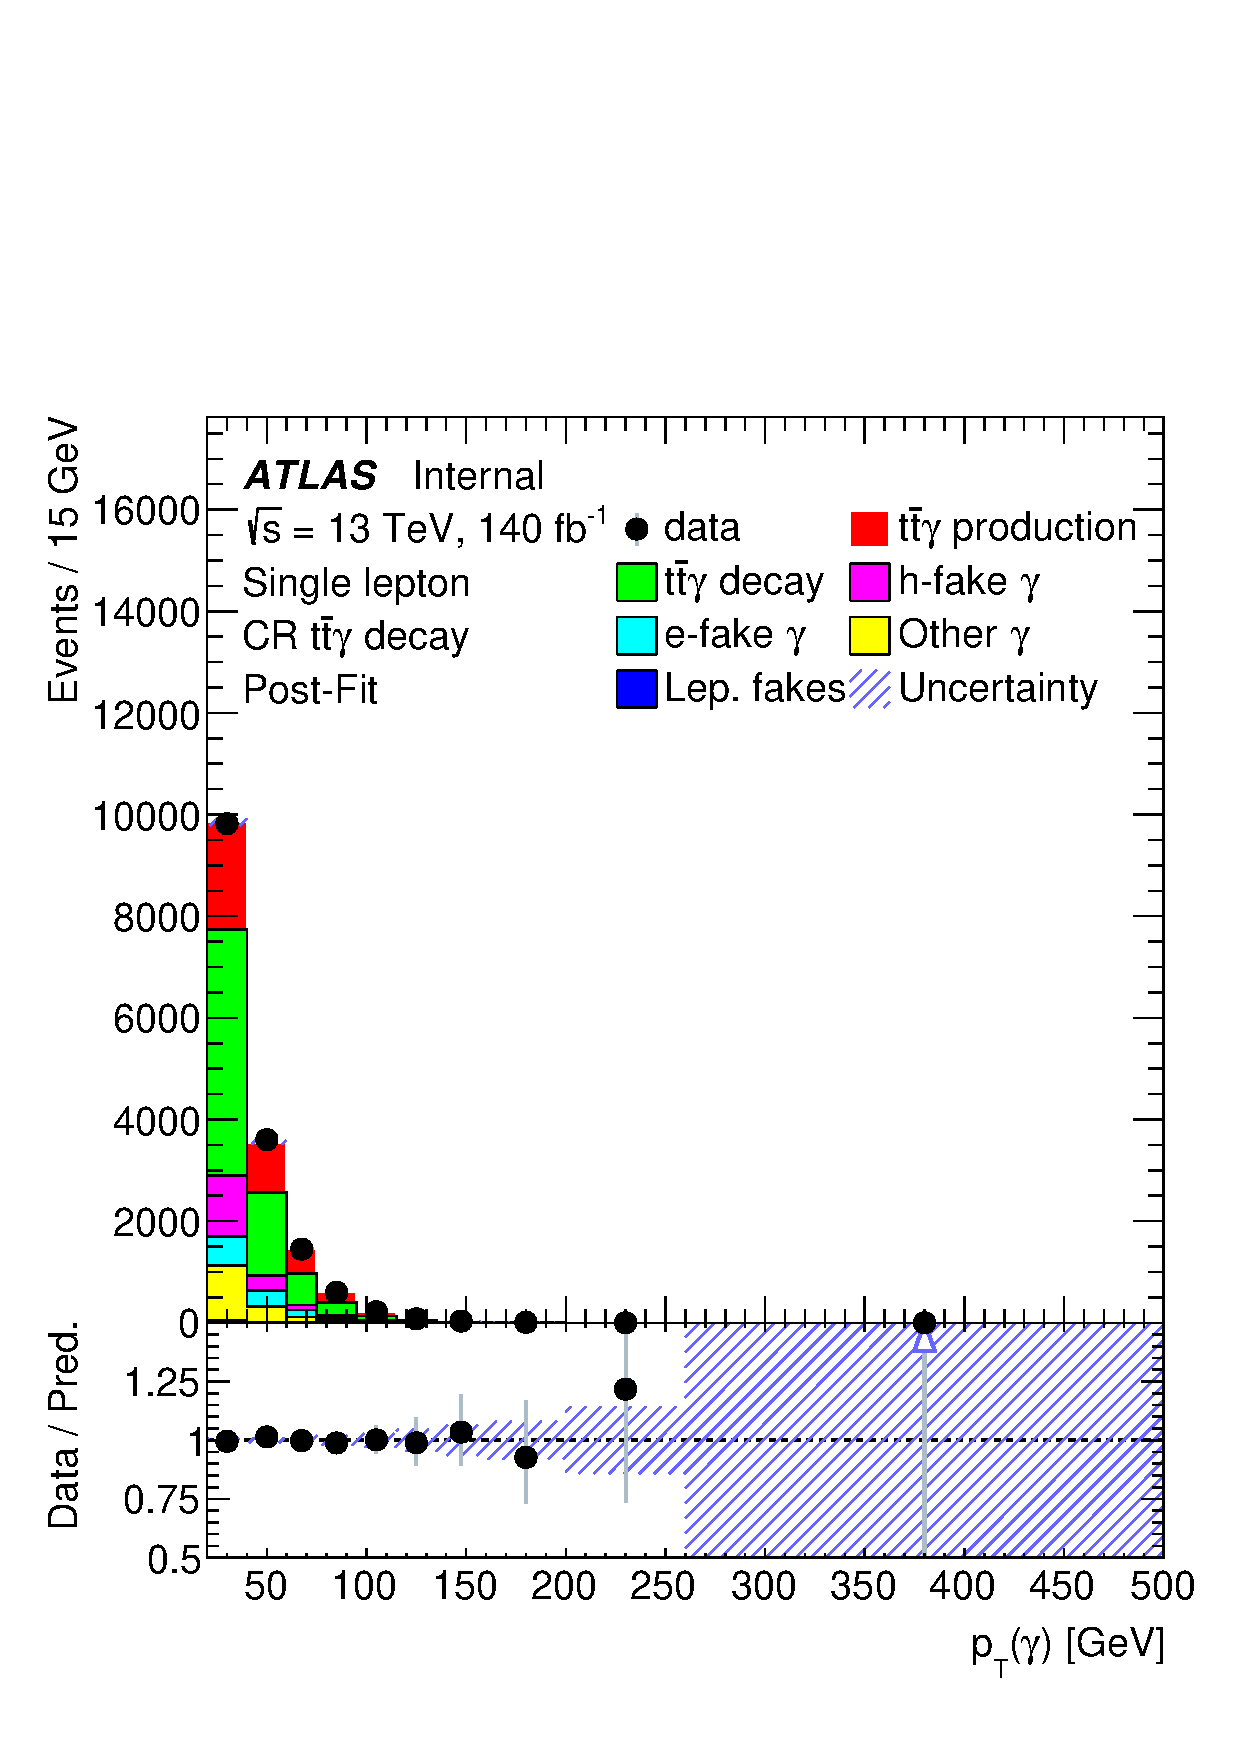
\includegraphics[width=0.30\textwidth]{figures/diff_xsec/ljet_dilep_combination_mu_blinded/post-fit/tty1l_pt_all_syst/SR2_ljet_postFit.pdf}}
  \quad\quad
  \subfloat[]{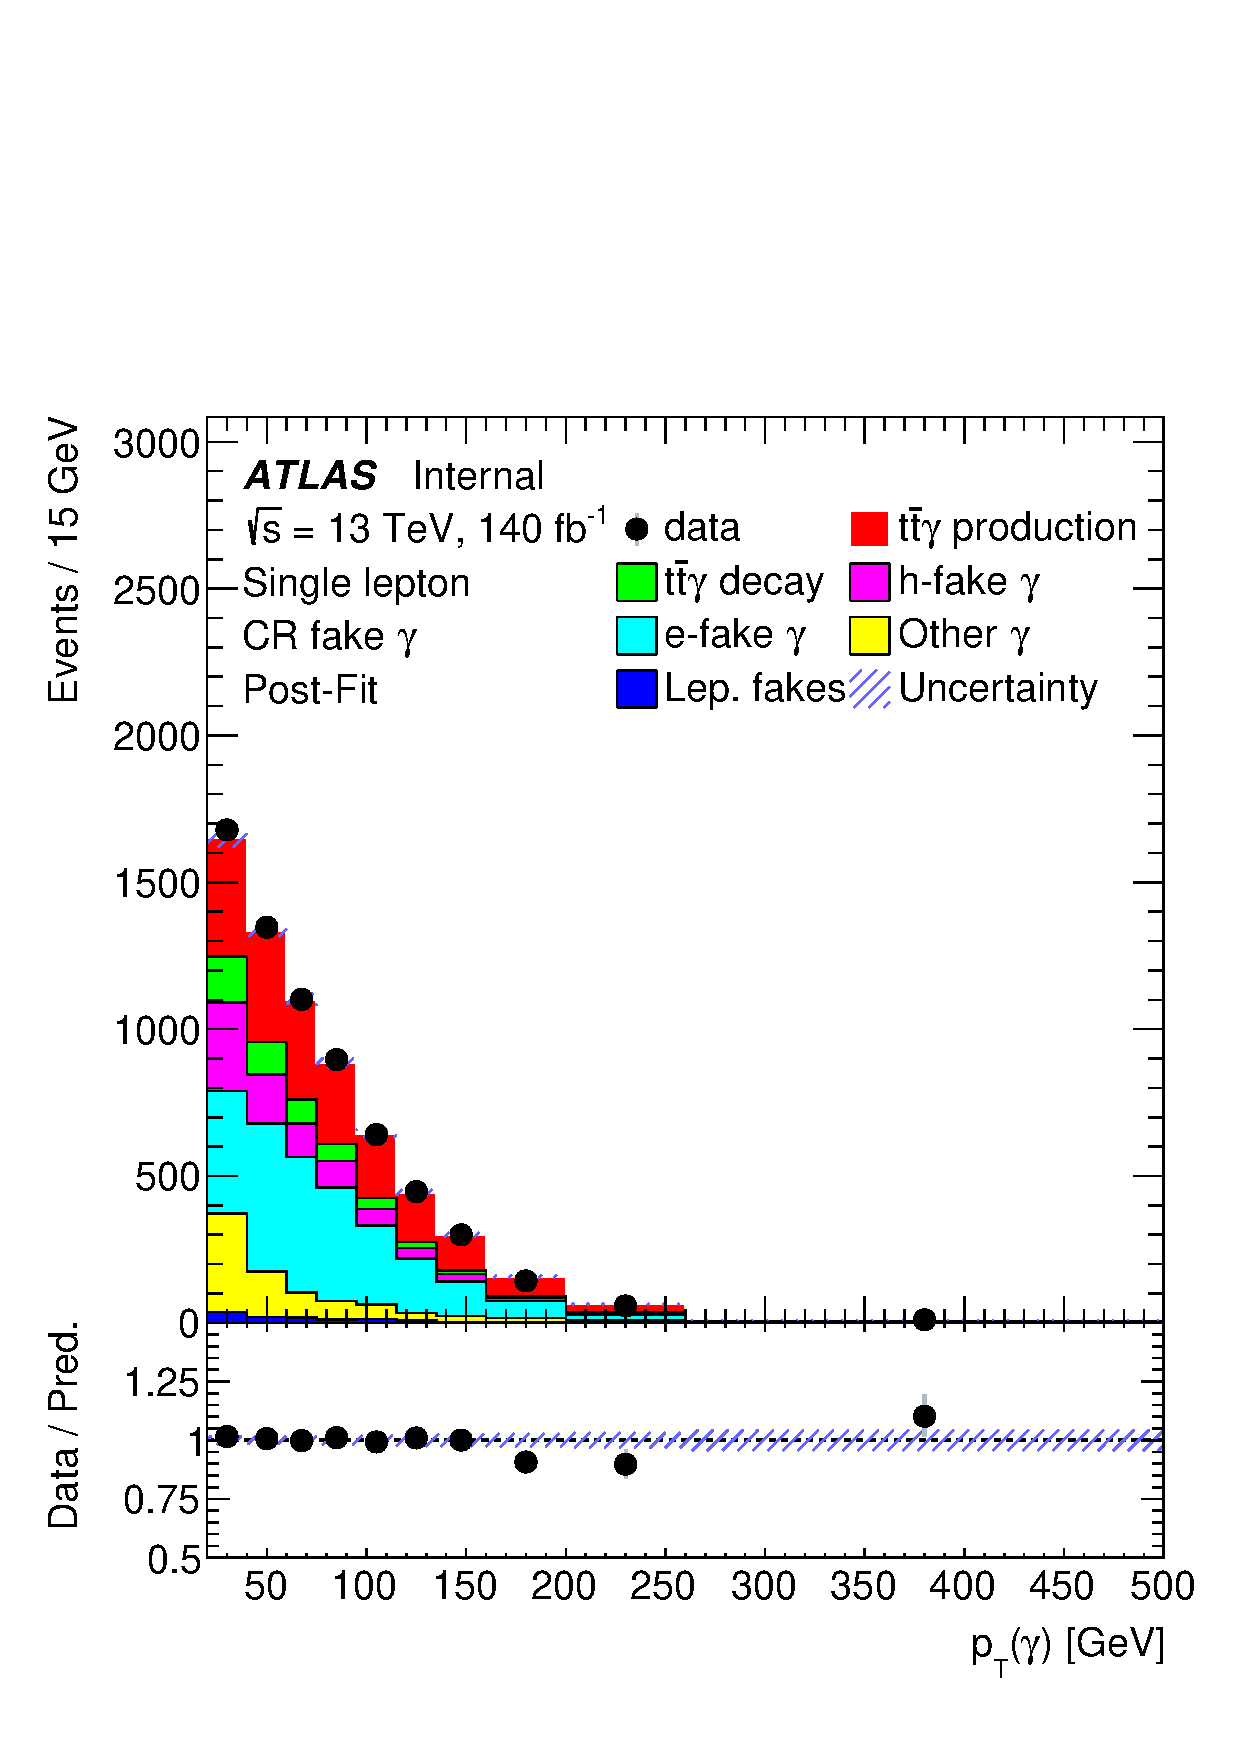
\includegraphics[width=0.30\textwidth]{figures/diff_xsec/ljet_dilep_combination_mu_blinded/post-fit/tty1l_pt_all_syst/SR3_ljet_postFit.pdf}}
  \quad\quad
  \subfloat[]{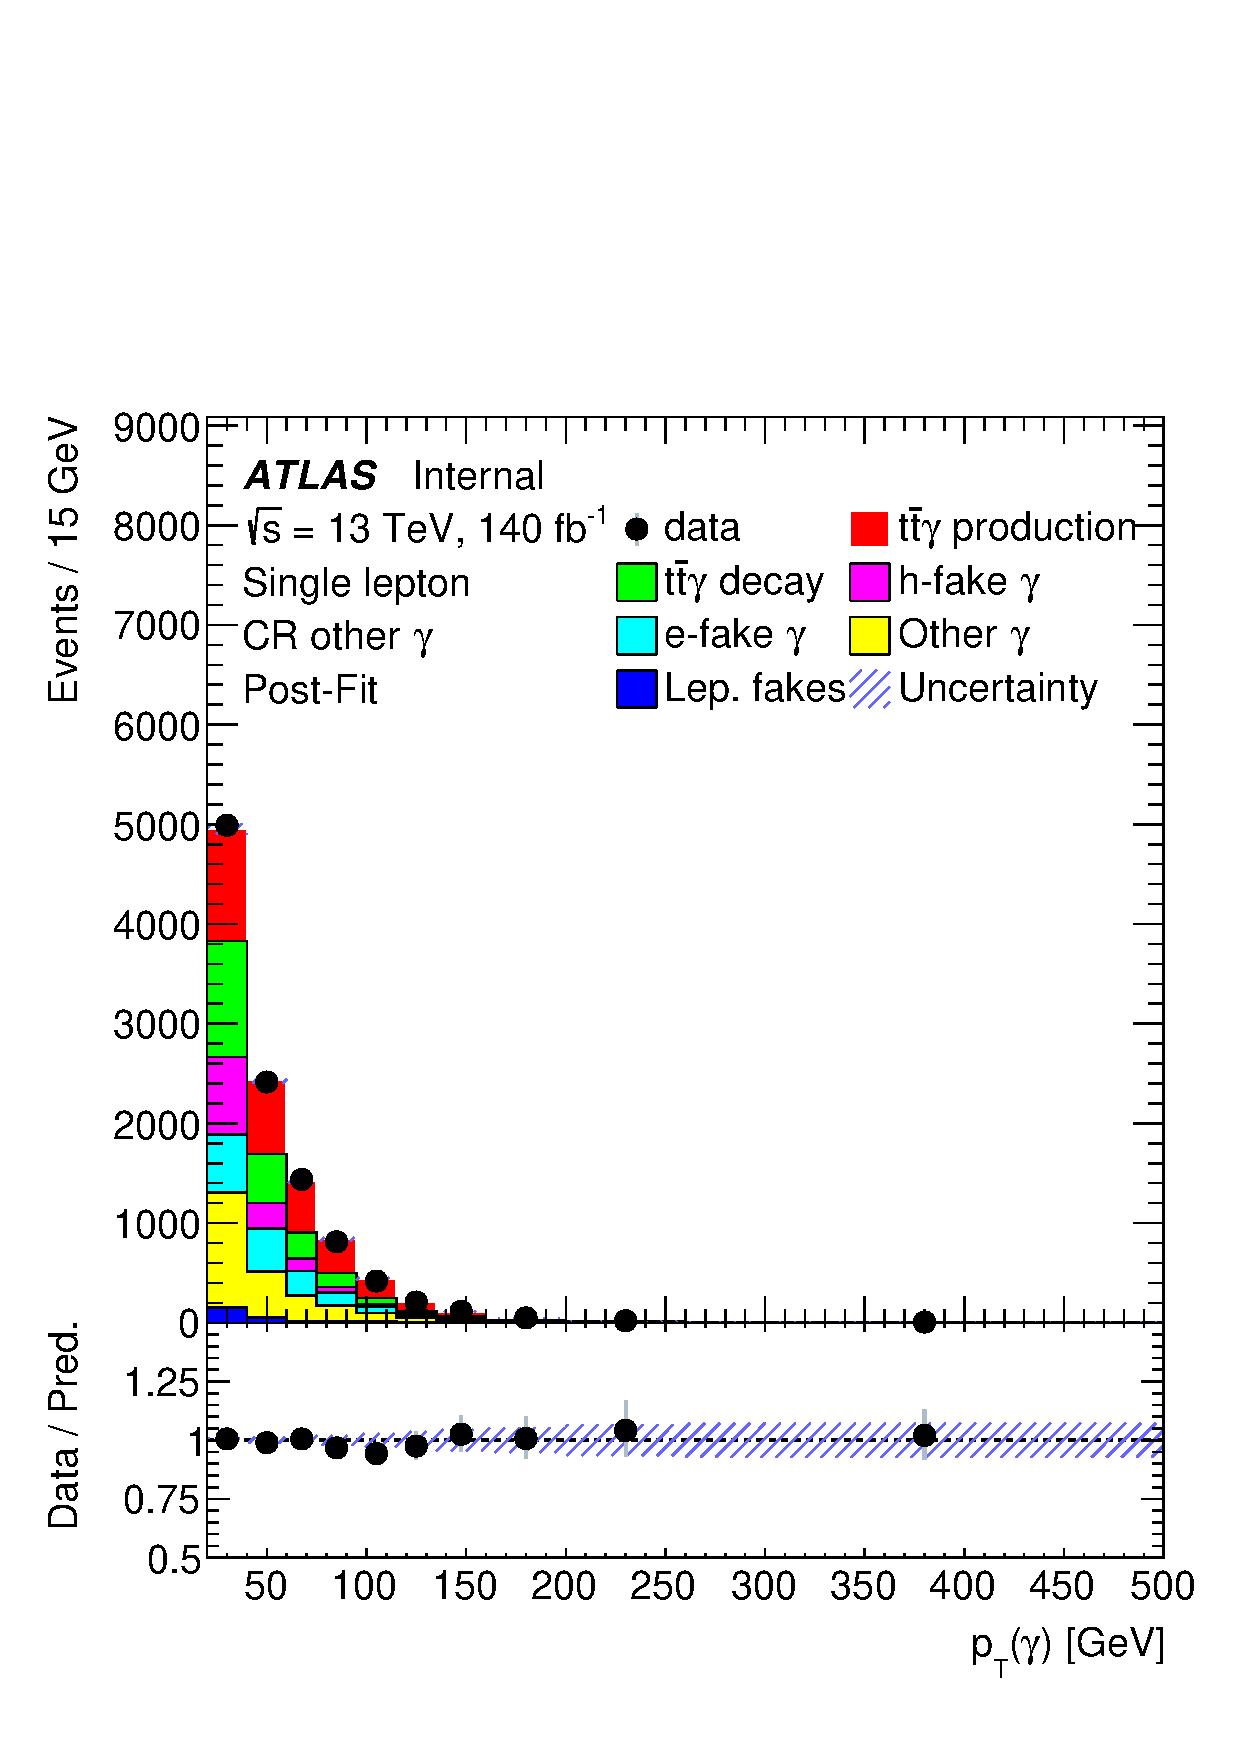
\includegraphics[width=0.30\textwidth]{figures/diff_xsec/ljet_dilep_combination_mu_blinded/post-fit/tty1l_pt_all_syst/SR4_ljet_postFit.pdf}}
  \quad \quad
  \subfloat[]{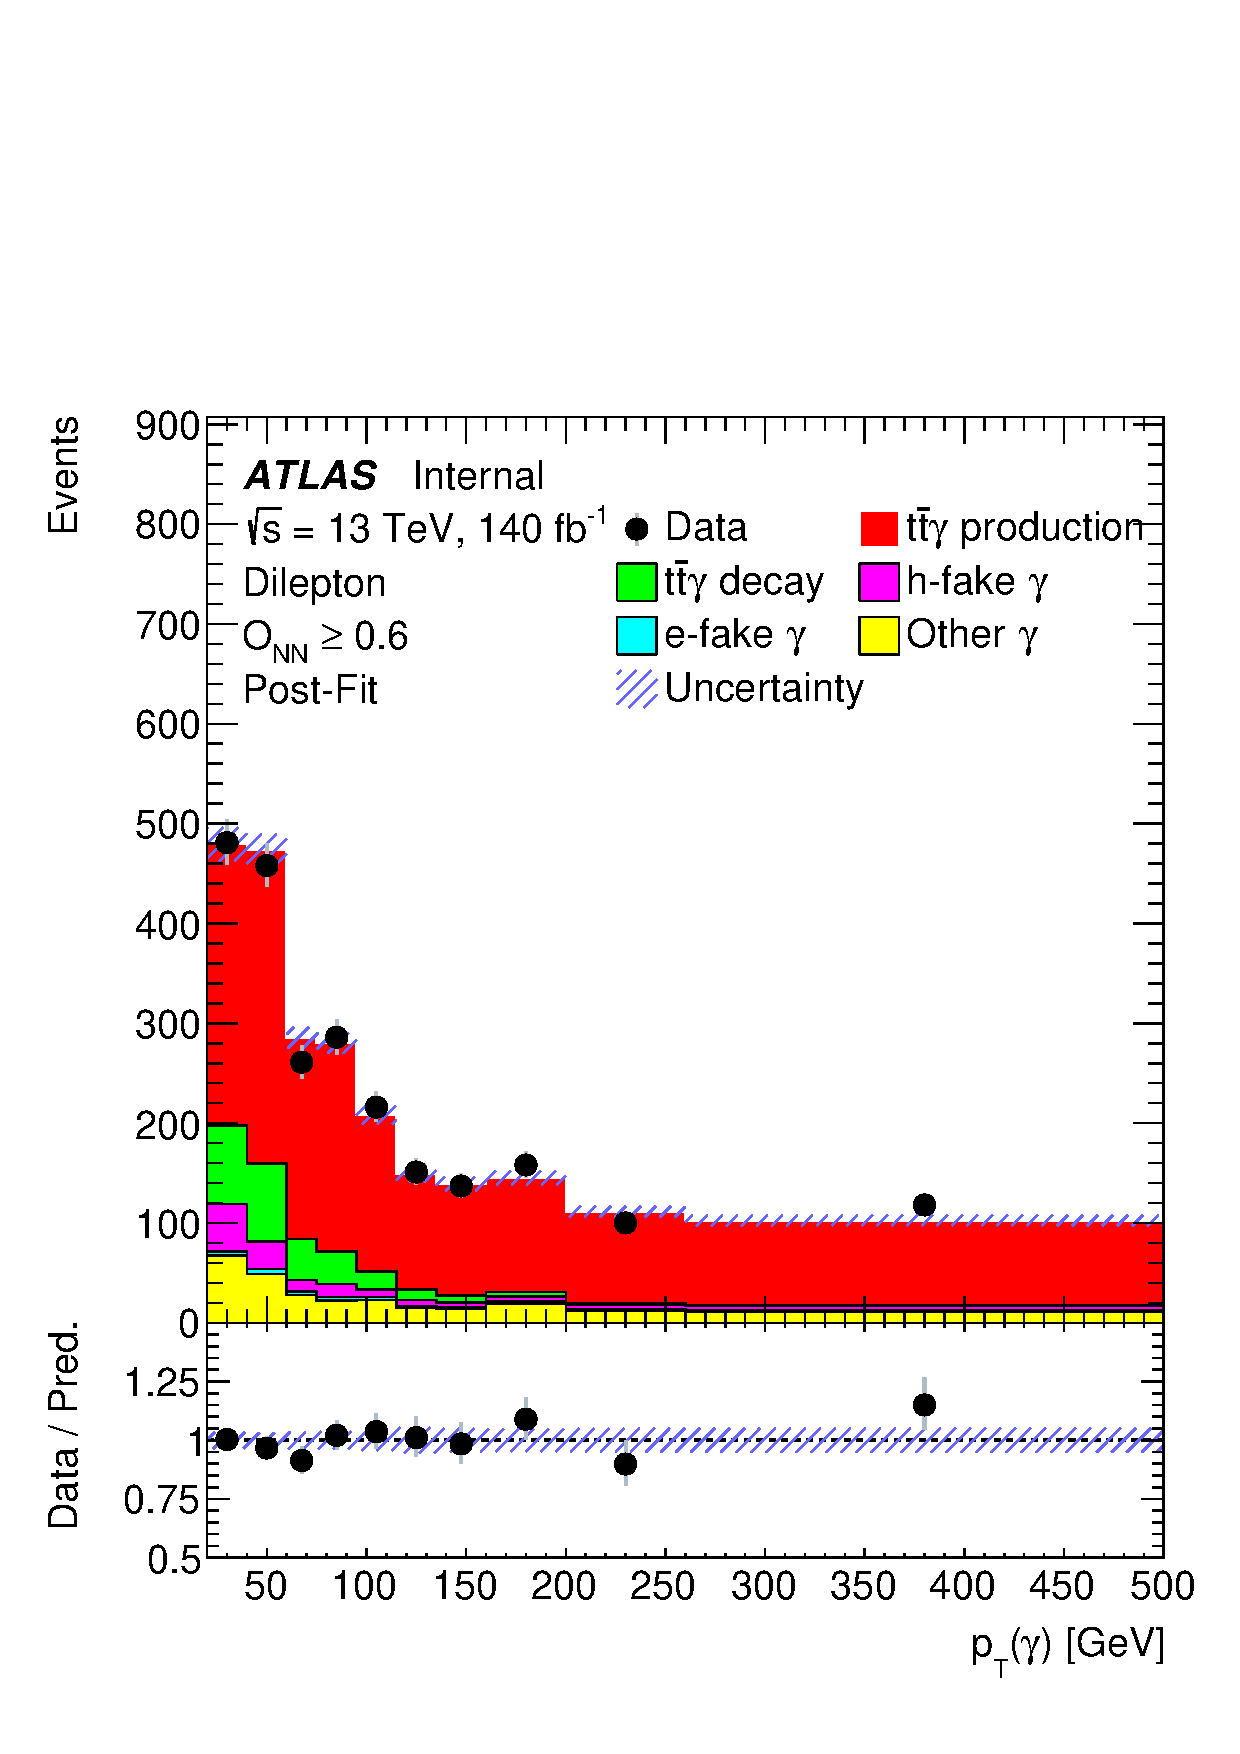
\includegraphics[width=0.30\textwidth]{figures/diff_xsec/ljet_dilep_combination_mu_blinded/post-fit/tty2l_pt_all_syst/SR1_dilep_postFit.pdf}}
  \quad\quad
  \subfloat[]{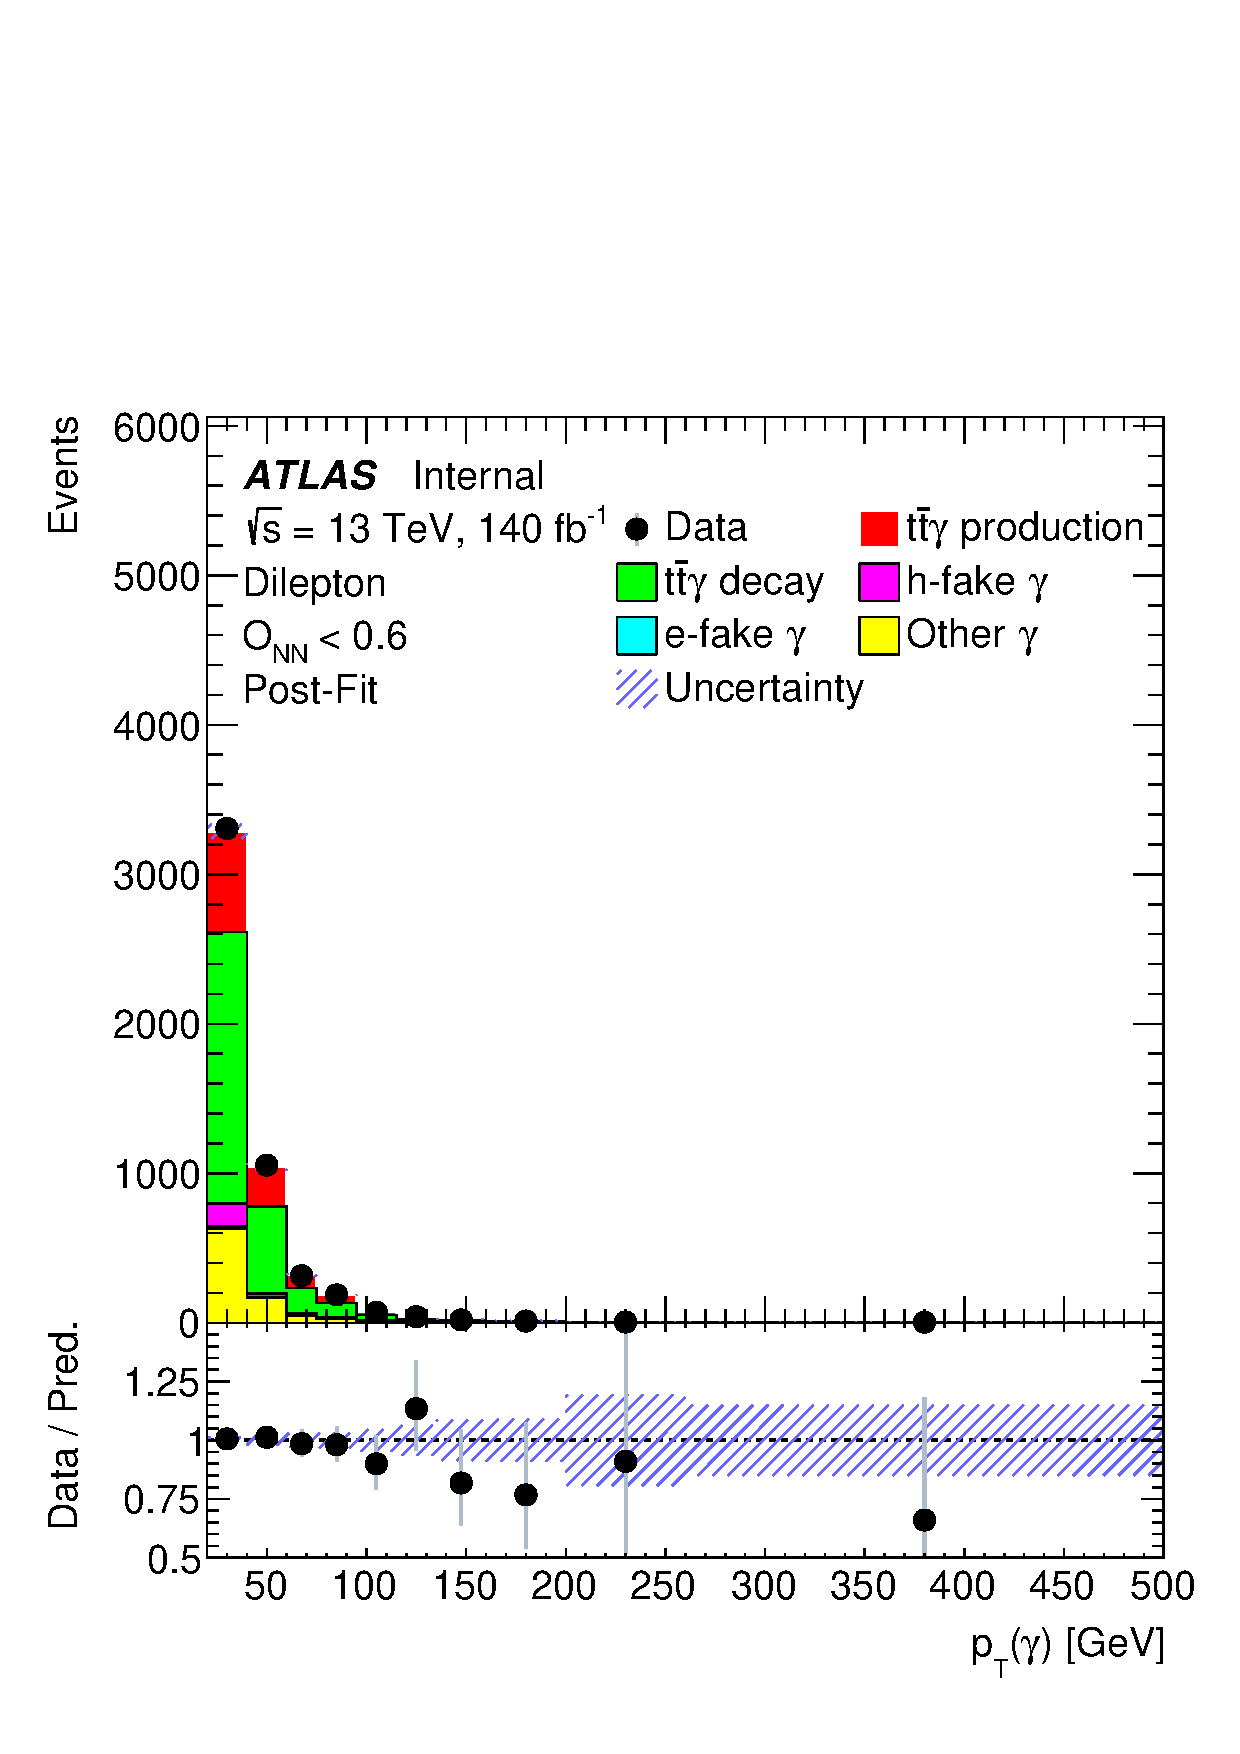
\includegraphics[width=0.30\textwidth]{figures/diff_xsec/ljet_dilep_combination_mu_blinded/post-fit/tty2l_pt_all_syst/SR2_dilep_postFit.pdf}}

  \caption{The post-fit distributions of $p_T(\gamma)$ in 4 regions ( (a) \tty (prod.) enriched region  (b) \tty (dec.) enriched region
  (c) fakes enriched region (d) prompt photon enriched region) in single lepton channel and 2 regions in dilepton channel. }
  \label{fig:pt_postfit_sldl_realdata}
\end{figure}
\FloatBarrier


\begin{figure}[ht]
  \centering
  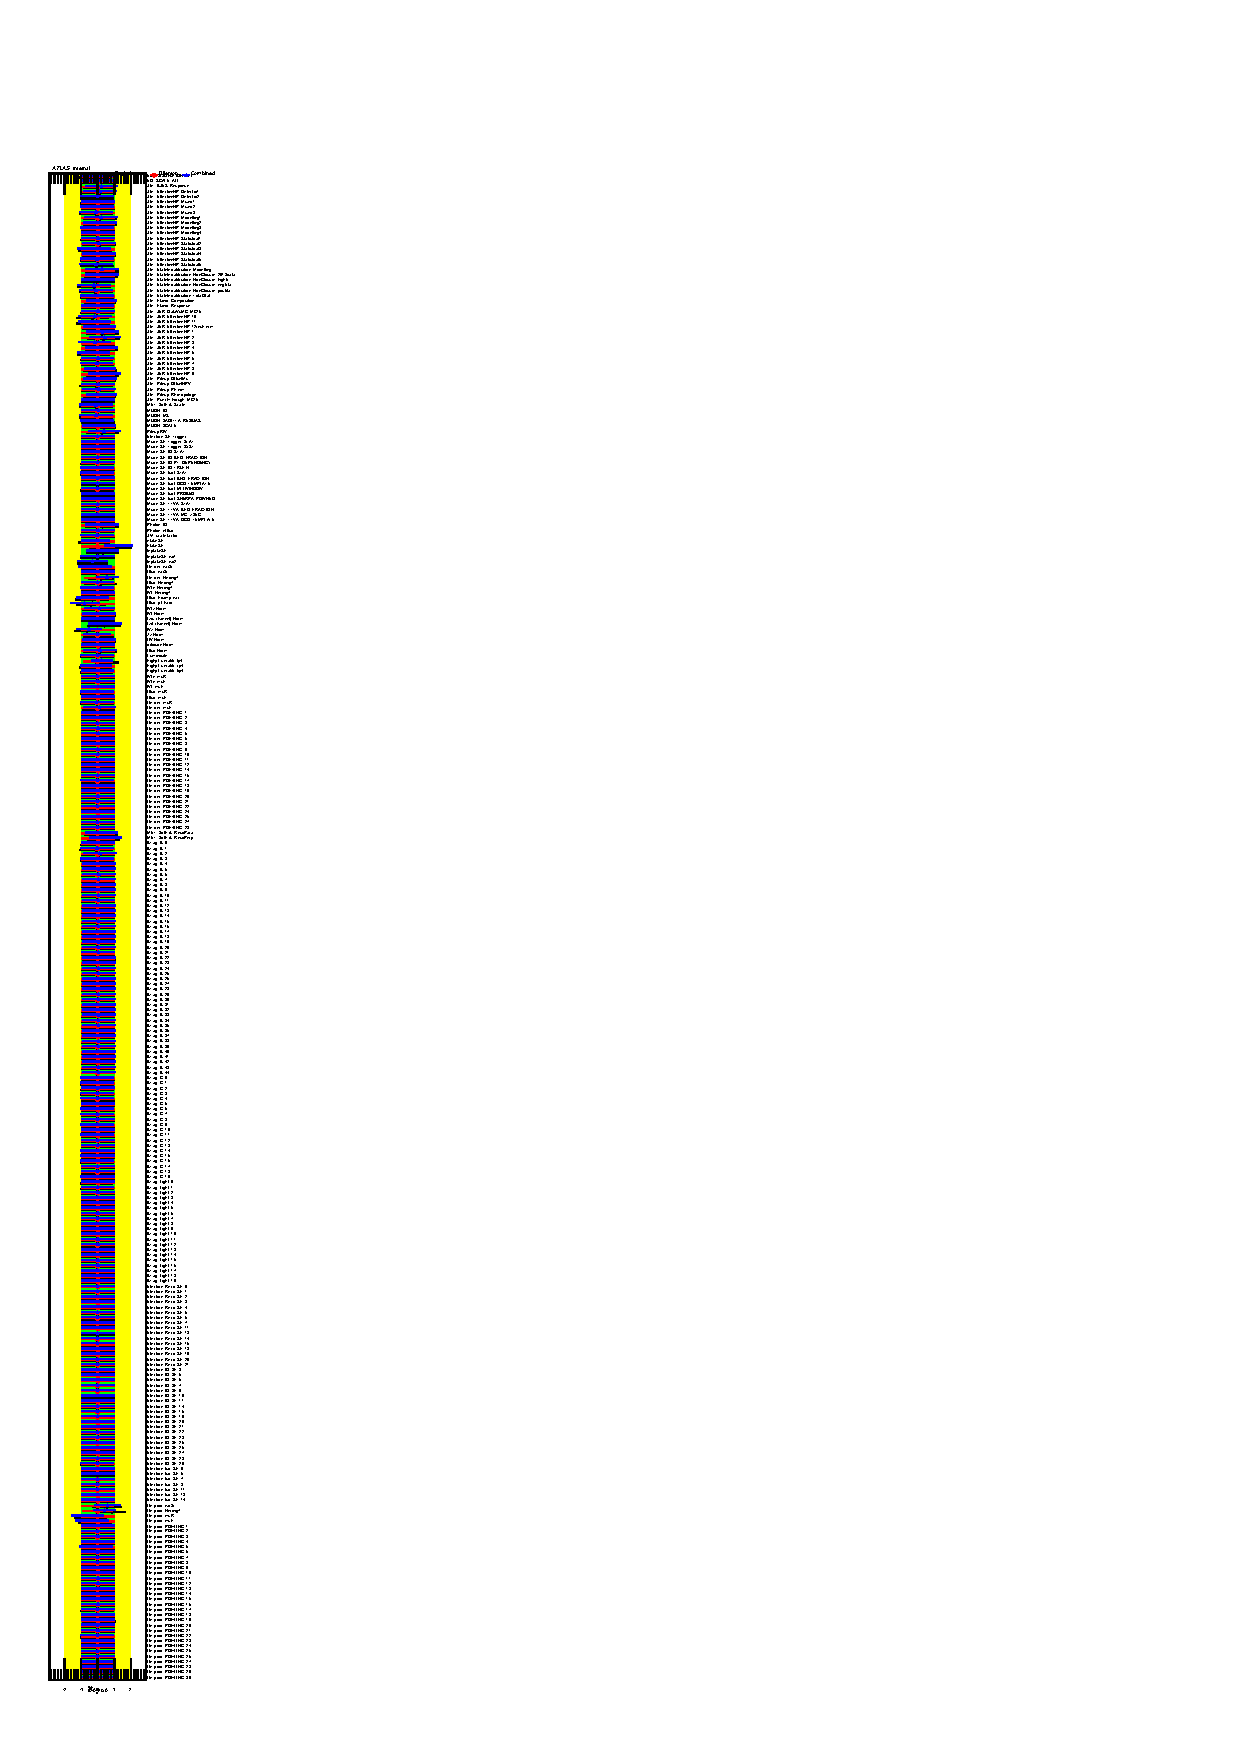
\includegraphics[width=0.20\textwidth]{figures/diff_xsec/ljet_dilep_combination_mu_blinded/compare_NP_pulls/tty_combi_NP_pull_ph_pt.pdf}
  \quad\quad
  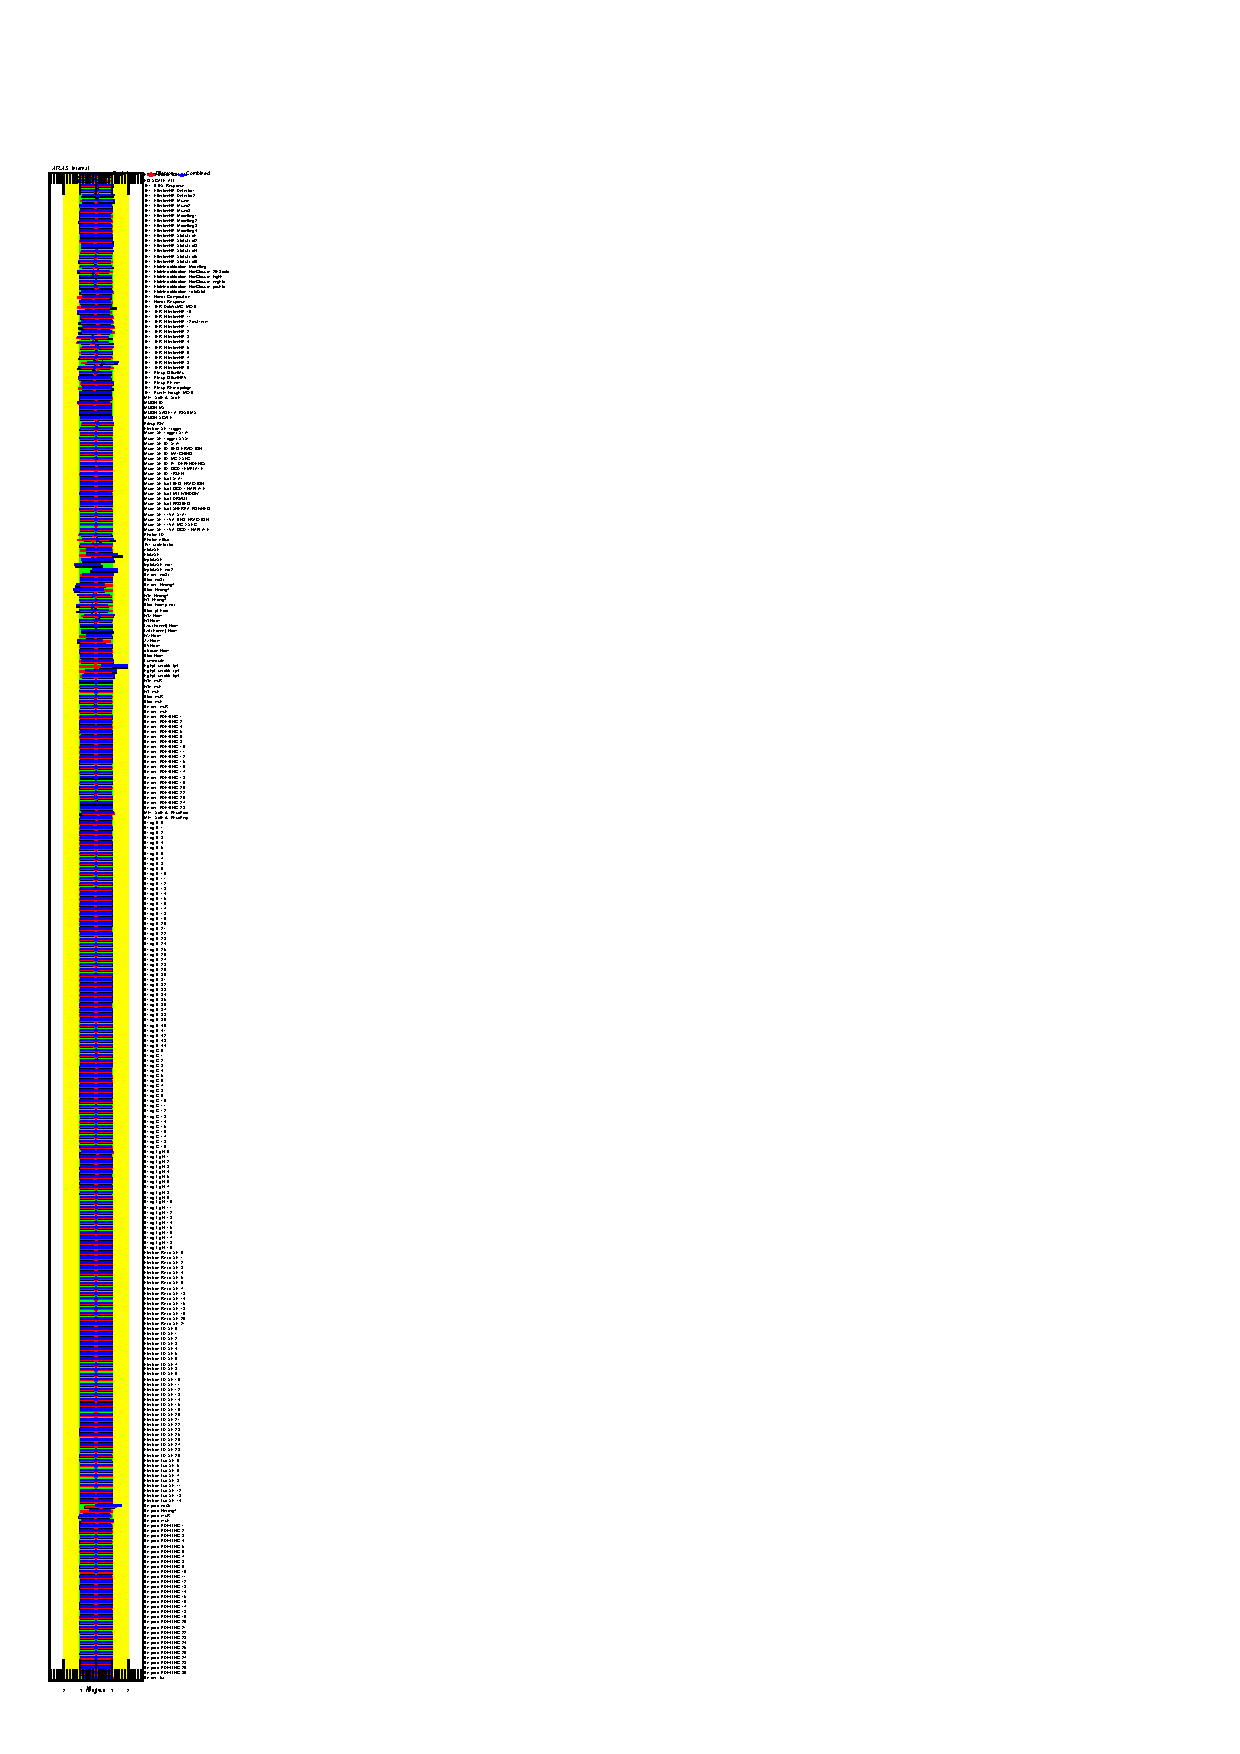
\includegraphics[width=0.20\textwidth]{figures/diff_xsec/ljet_dilep_combination_mu_blinded/compare_NP_pulls/tty_combi_NP_pull_ph_eta.pdf}
  \caption{Pull plots obtained from the fit to the data for the single lepton and dilepton combined channel, for the \tty production measurement.}
  \label{fig:pull_plot_pt_sldl_mu_blinded_tty_prod}
\end{figure}
\FloatBarrier

\begin{figure}[ht]
  \centering
  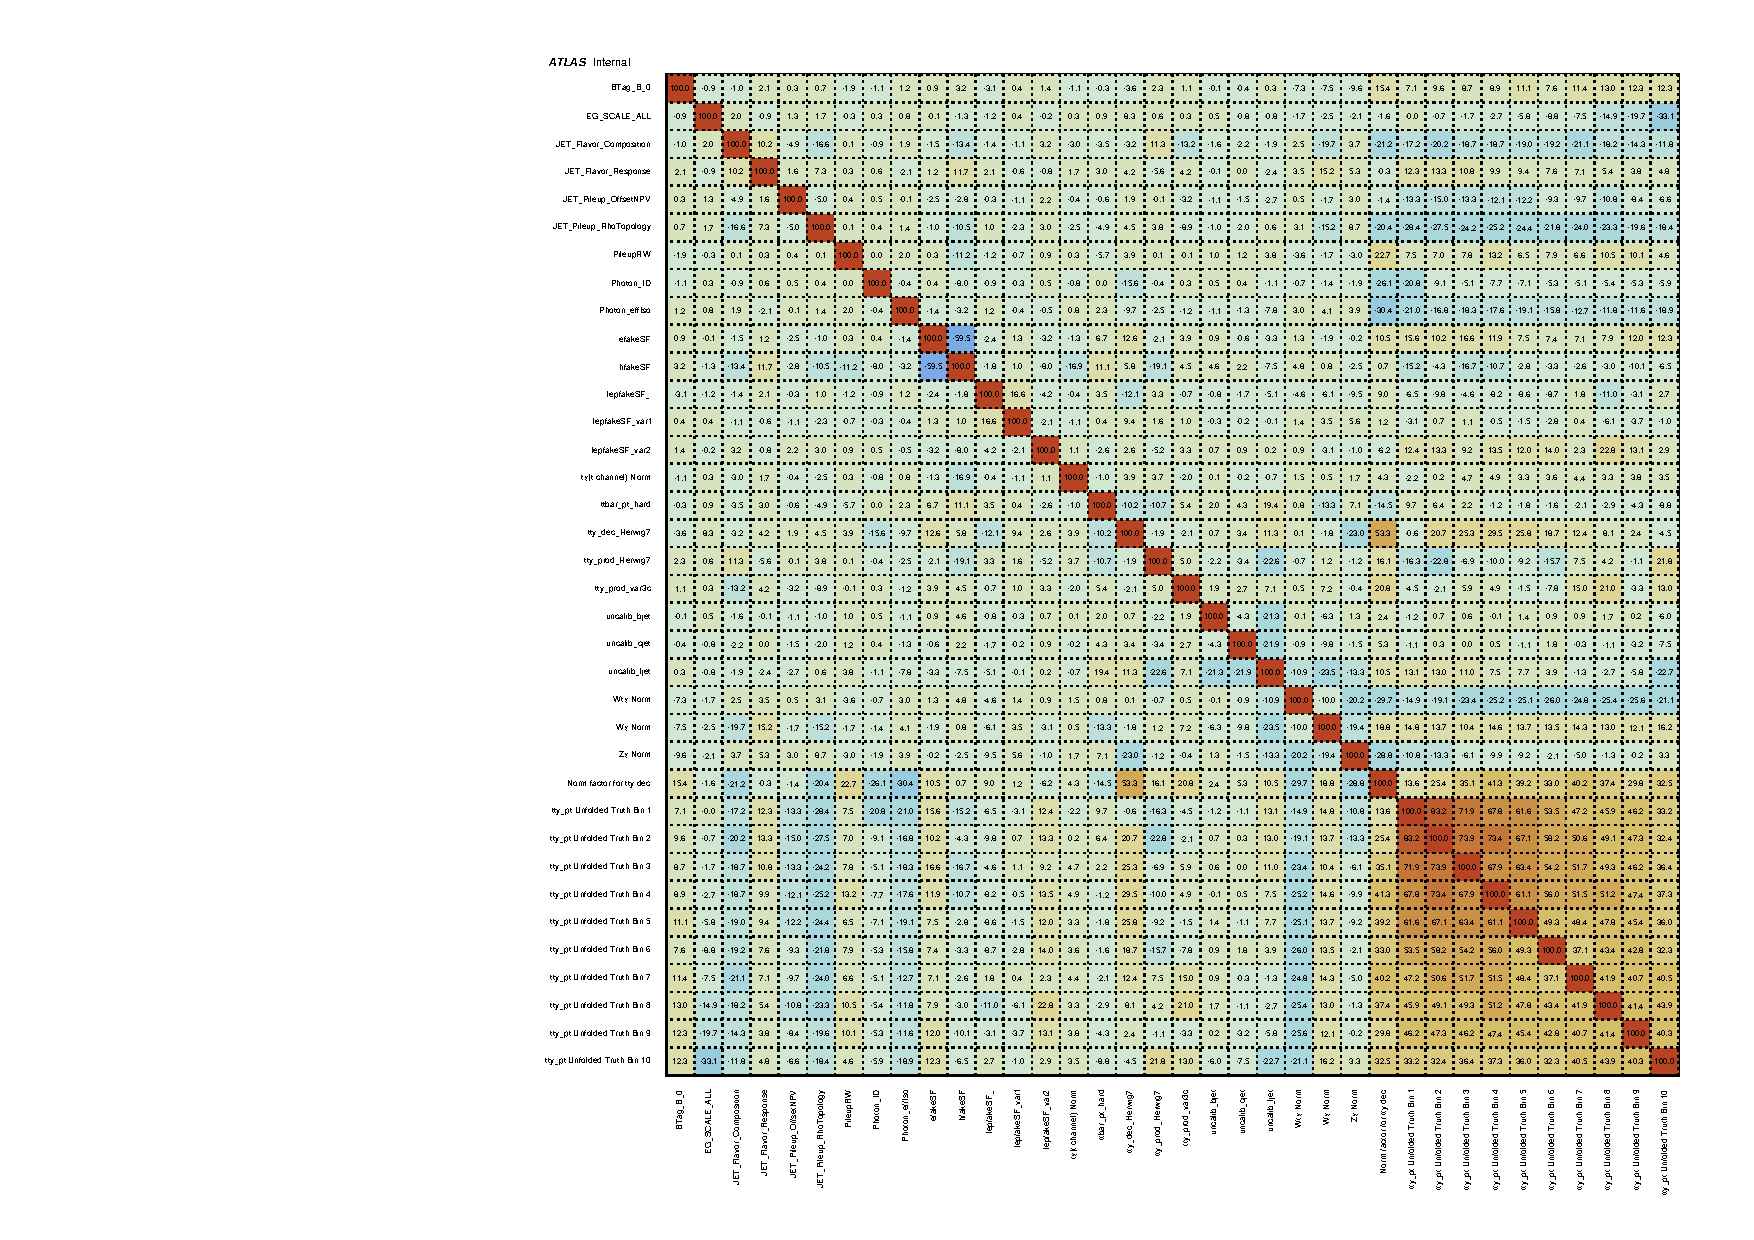
\includegraphics[width=0.6\textwidth]{figures/diff_xsec/ljet_dilep_combination_mu_blinded/correlations/tty_combi_corr_ph_pt.pdf}
  \quad\quad
  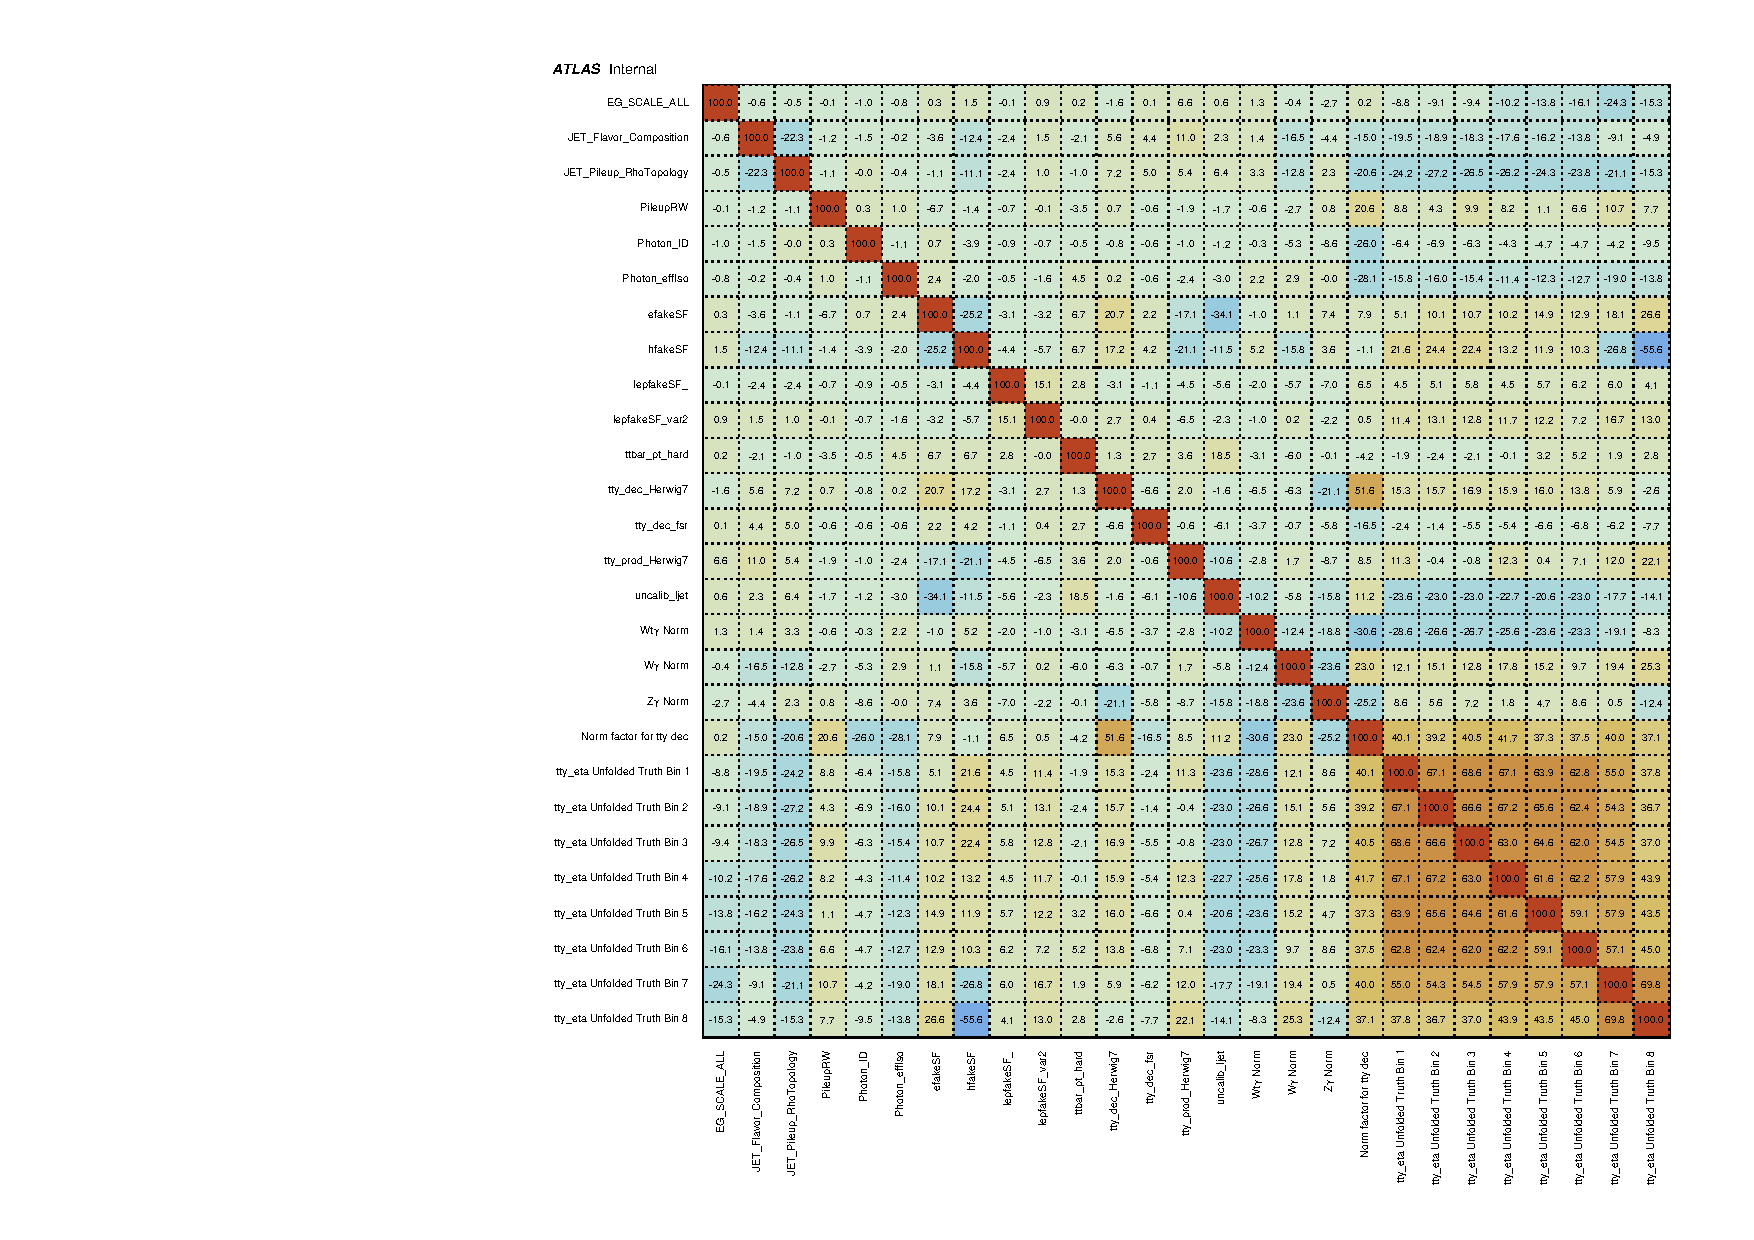
\includegraphics[width=0.6\textwidth]{figures/diff_xsec/ljet_dilep_combination_mu_blinded/correlations/tty_combi_corr_ph_eta.pdf}
  \caption{The correlation between the NPs and POIs for the measurement of 
  the $p_T(\gamma)$ distribution in the combined single lepton and dilepton channel for the \tty production measurement.}
  \label{fig:NP-corr_sldl_mu_blinded_tty_prod}
\end{figure}
\FloatBarrier

%%%%%%%%%%%% RANKING %%%%%%%%%%%%%%%%%%%

\begin{figure}[ht]
  \centering
  \subfloat[]{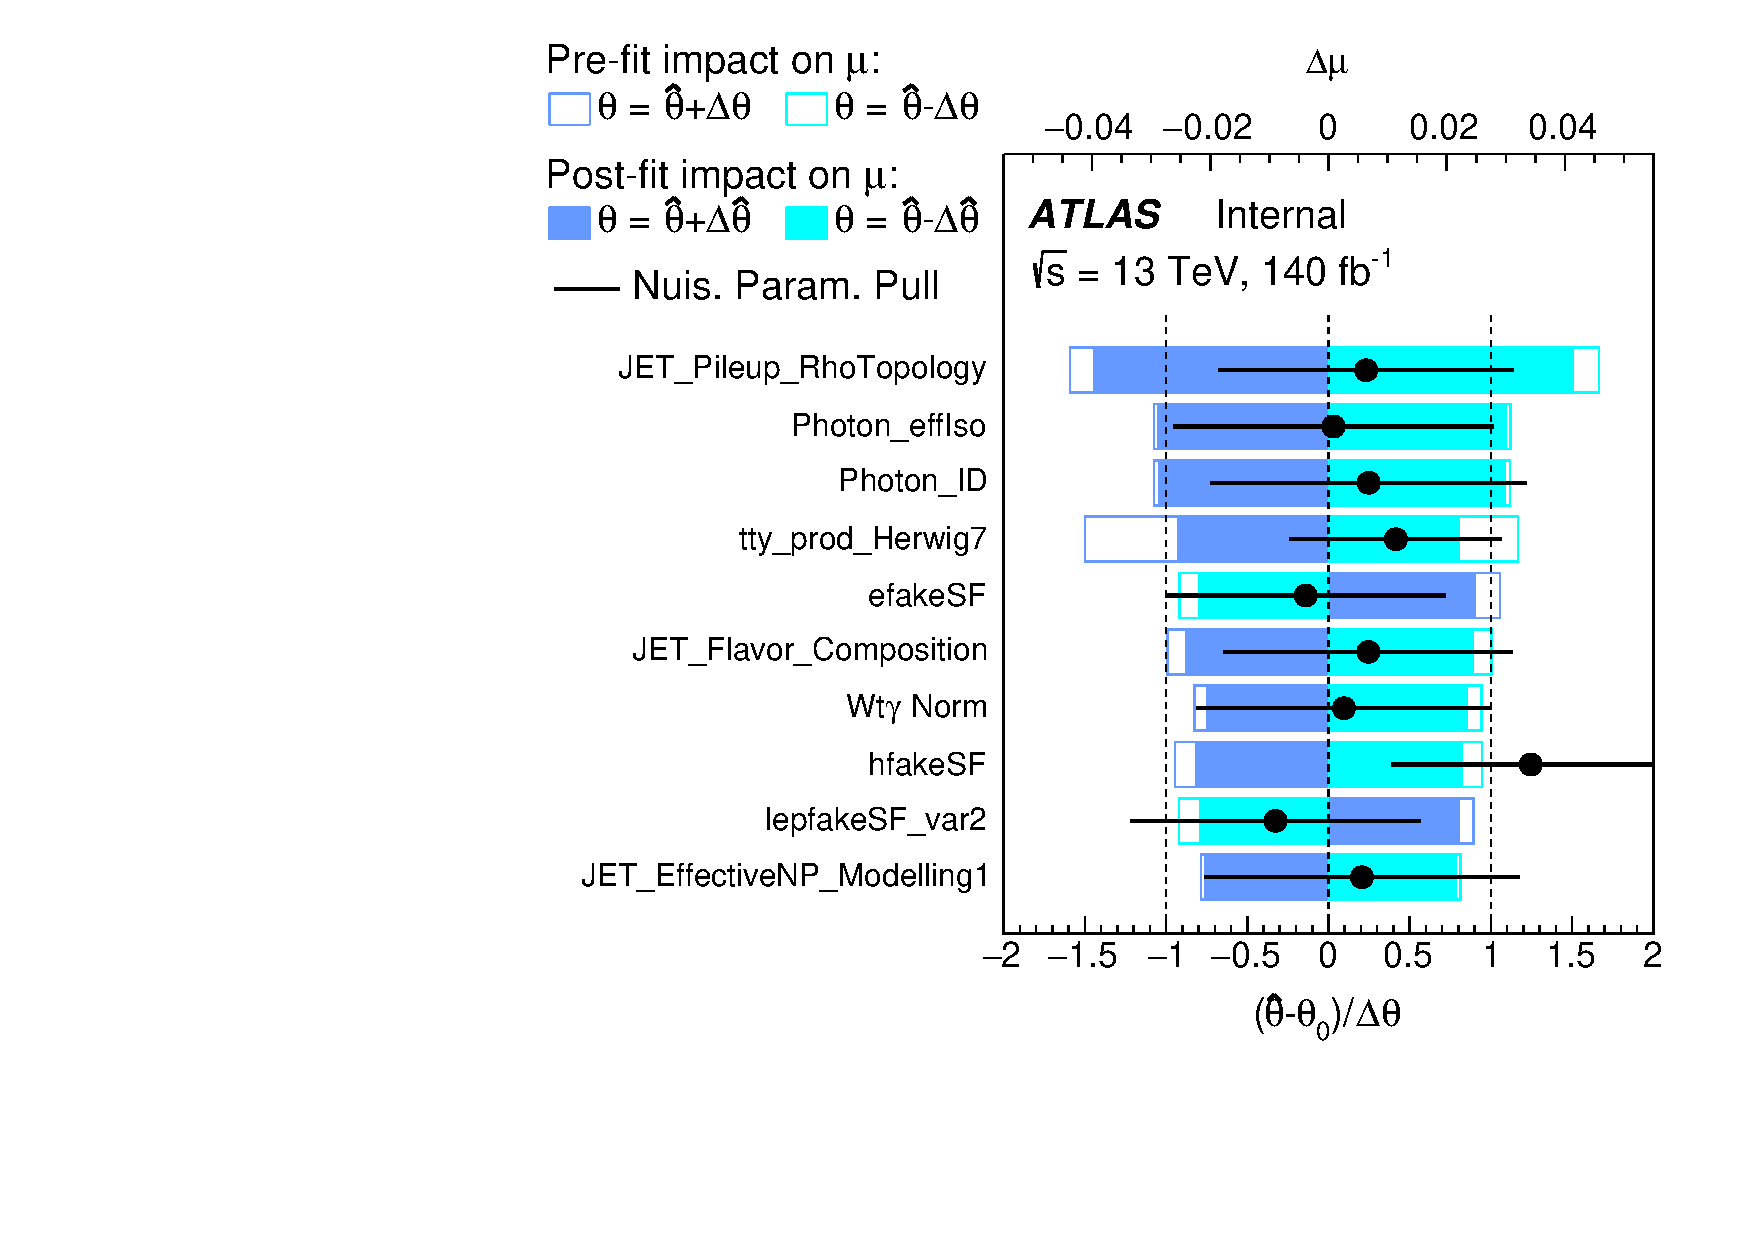
\includegraphics[width=0.2\textwidth]{figures/diff_xsec/ljet_dilep_combination_mu_blinded/Ranking/Ranking_tty_pt_Bin_001_mu.pdf}}
  \quad \quad
  \subfloat[]{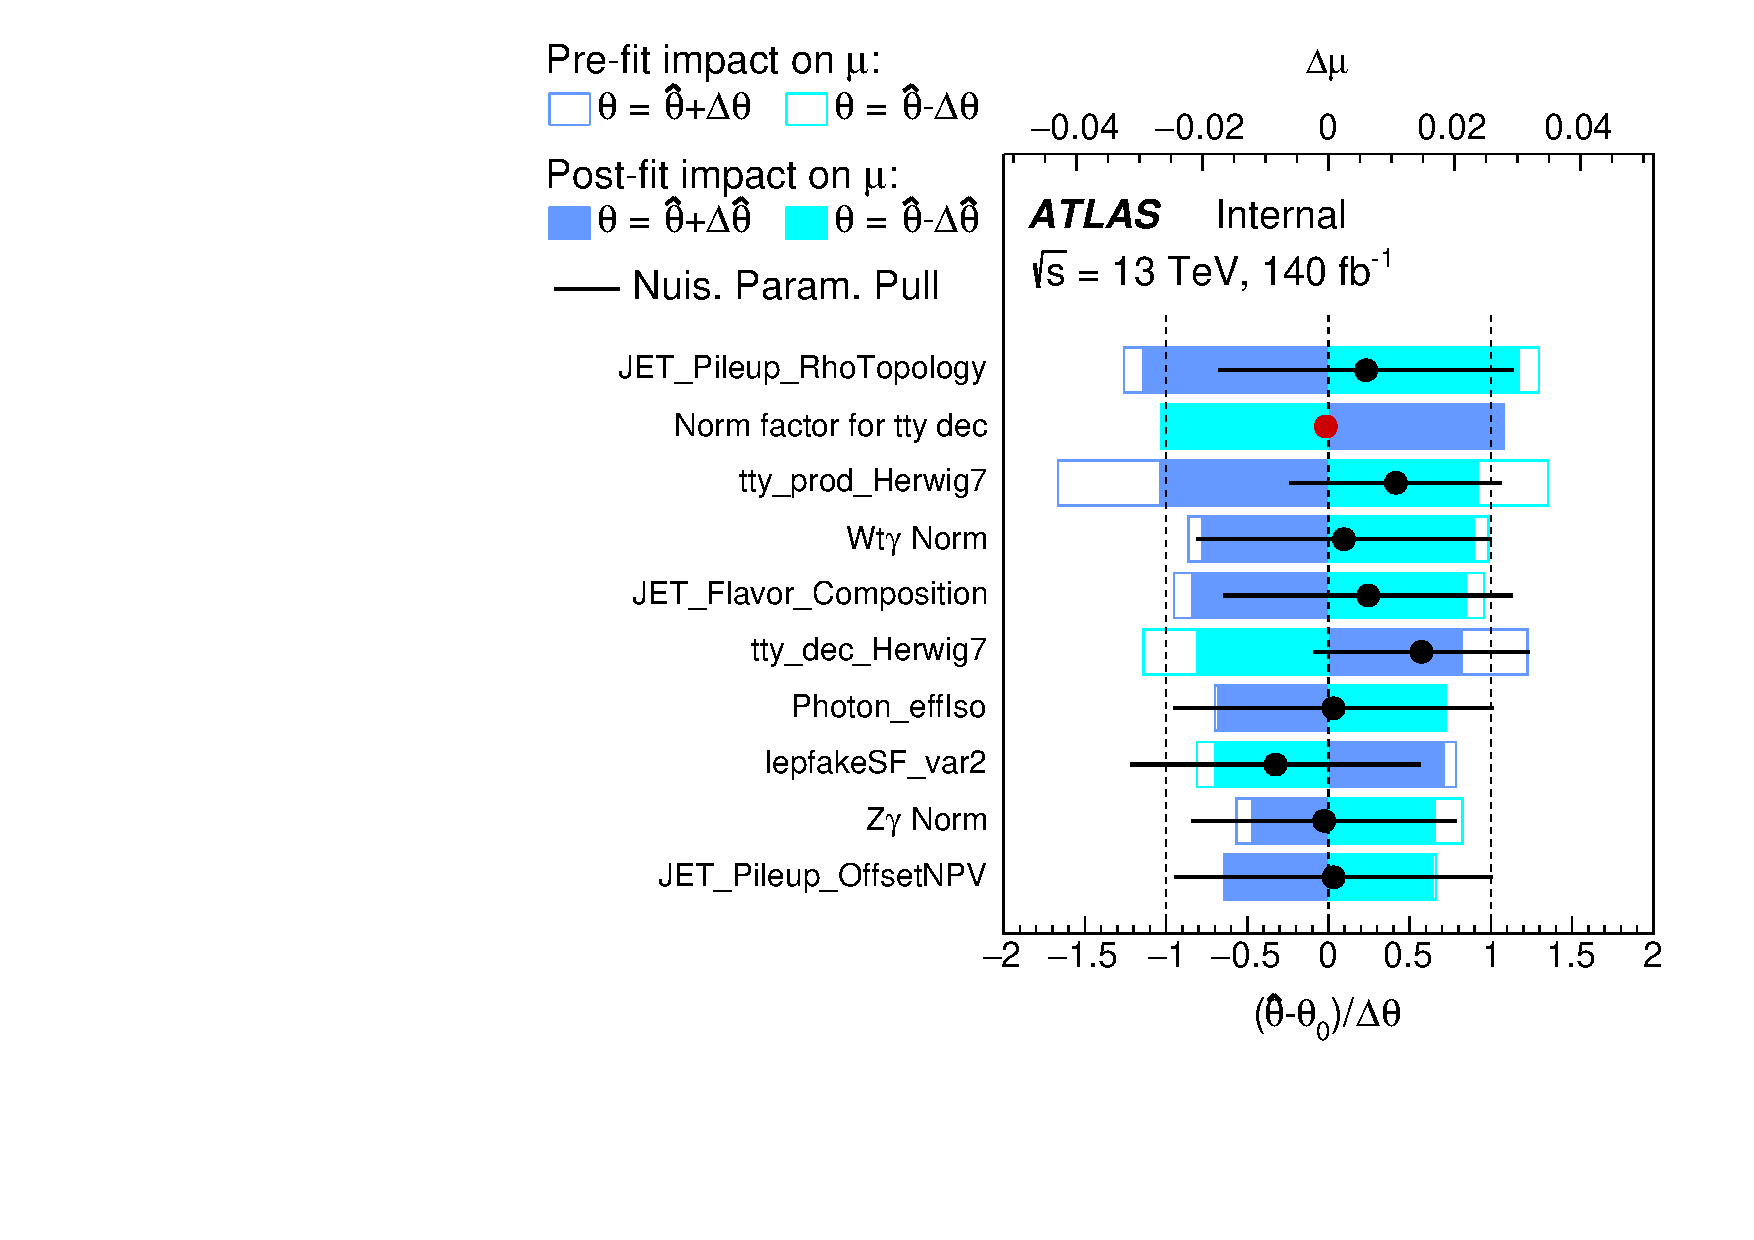
\includegraphics[width=0.2\textwidth]{figures/diff_xsec/ljet_dilep_combination_mu_blinded/Ranking/Ranking_tty_pt_Bin_002_mu.pdf}}
  \quad \quad
  \subfloat[]{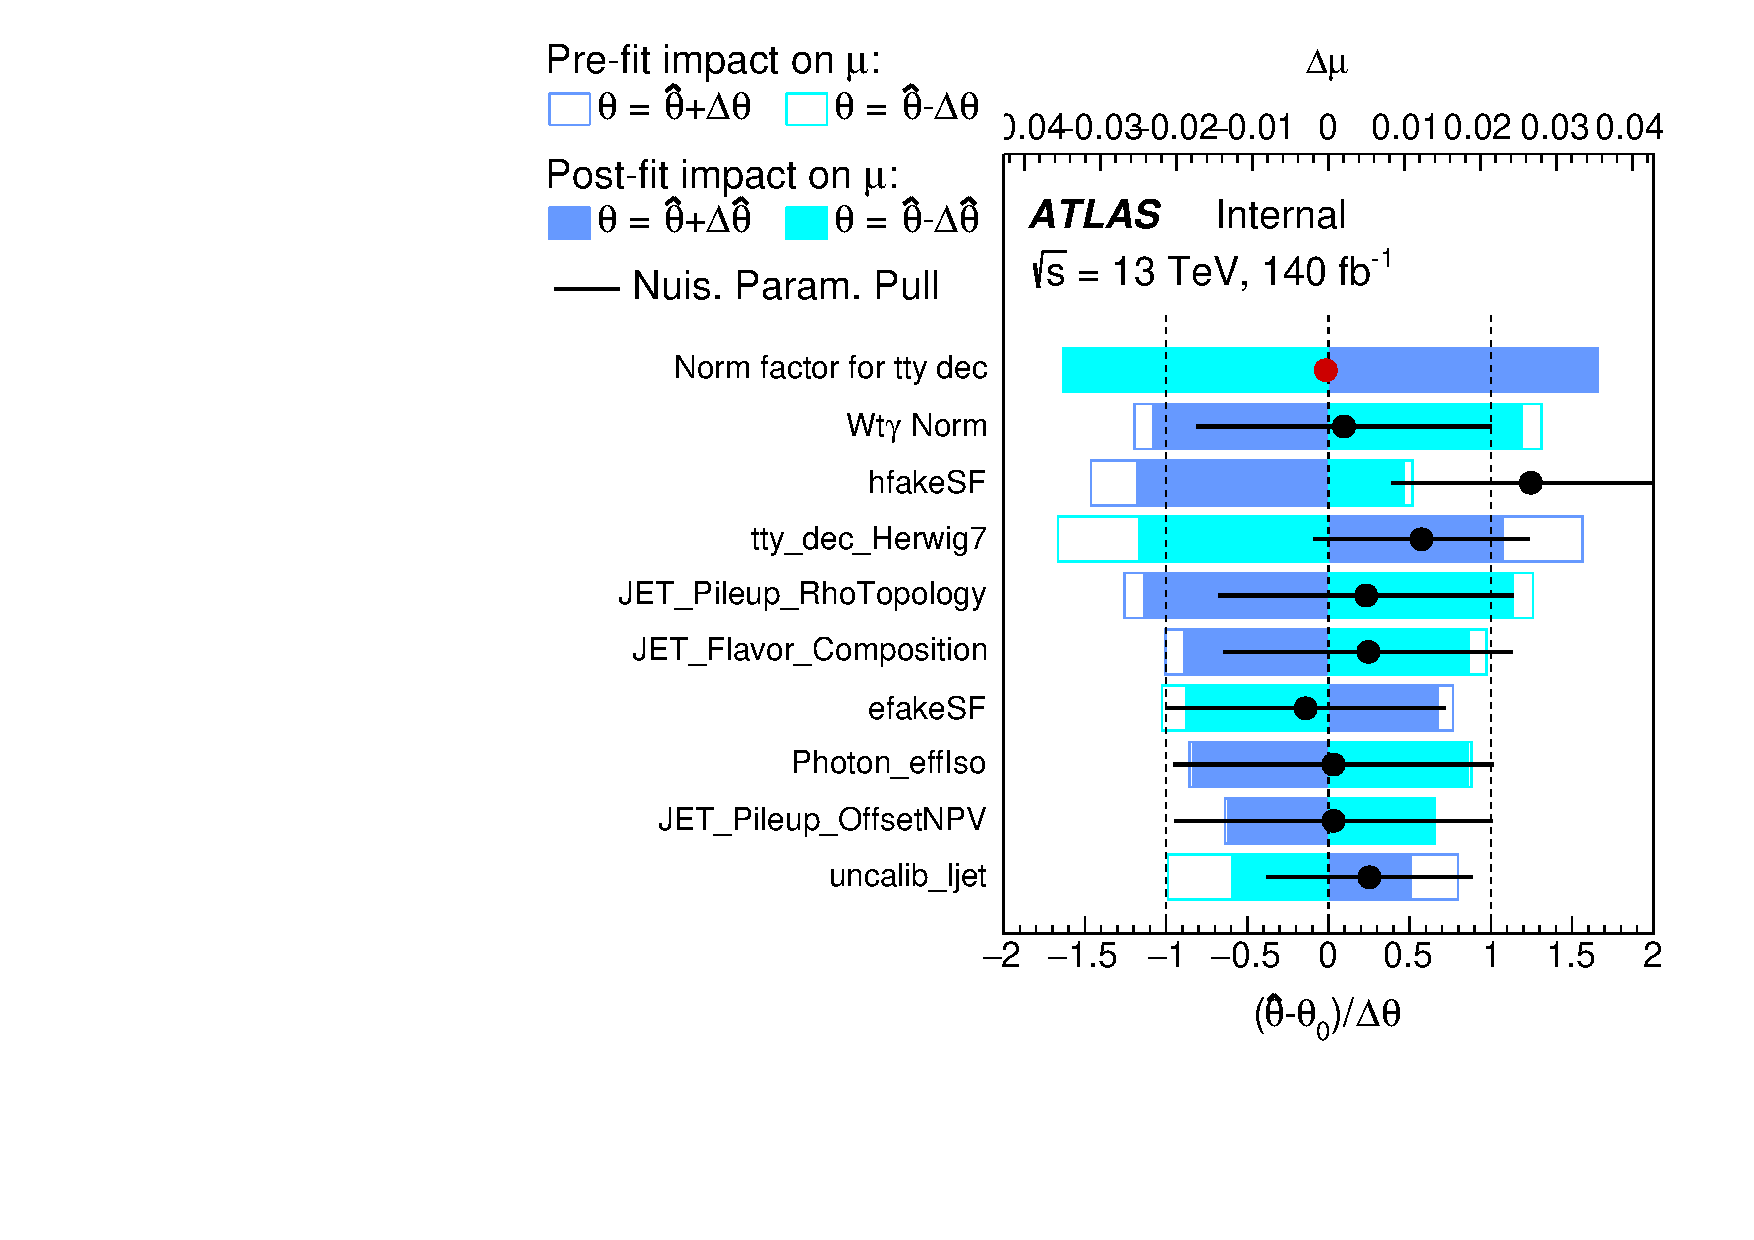
\includegraphics[width=0.2\textwidth]{figures/diff_xsec/ljet_dilep_combination_mu_blinded/Ranking/Ranking_tty_pt_Bin_003_mu.pdf}}
  \quad \quad
  \subfloat[]{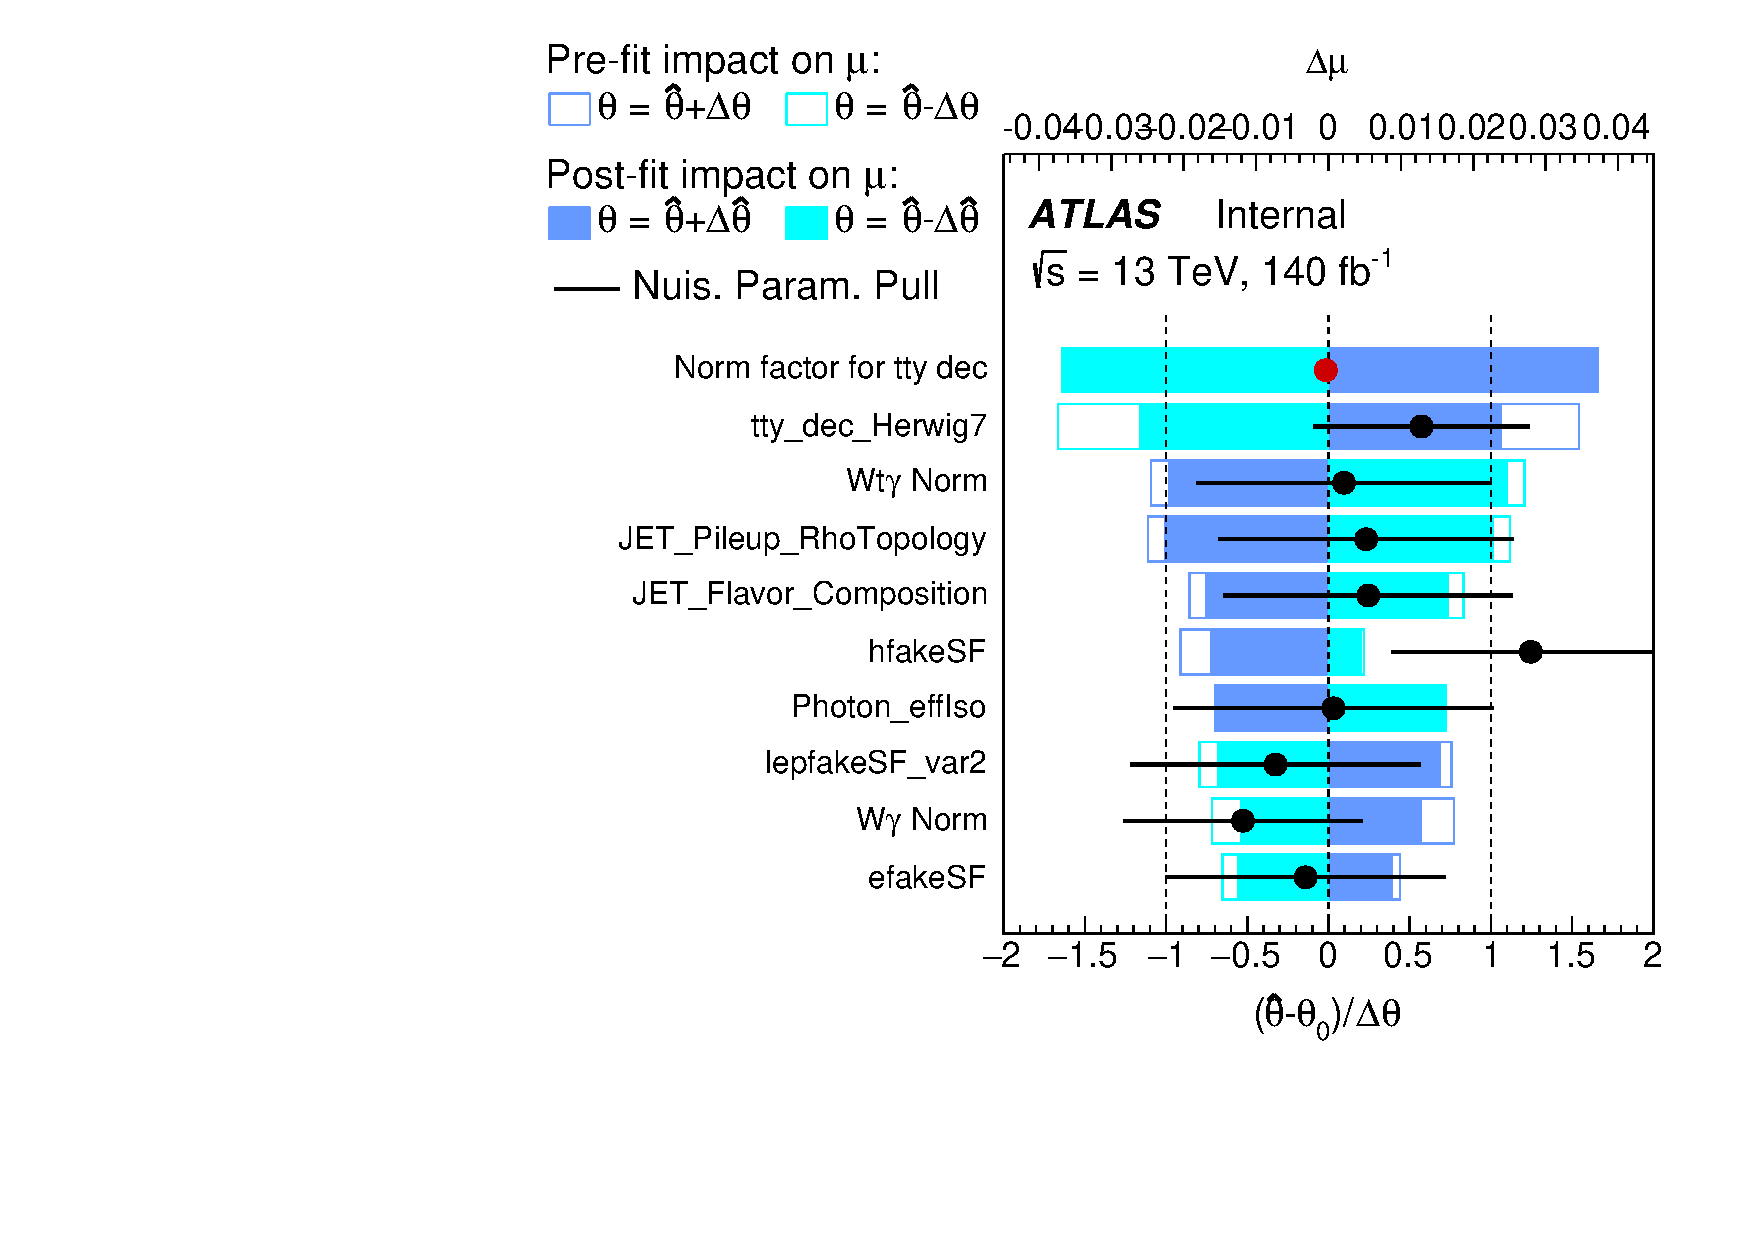
\includegraphics[width=0.2\textwidth]{figures/diff_xsec/ljet_dilep_combination_mu_blinded/Ranking/Ranking_tty_pt_Bin_004_mu.pdf}}
  \quad \quad
  \subfloat[]{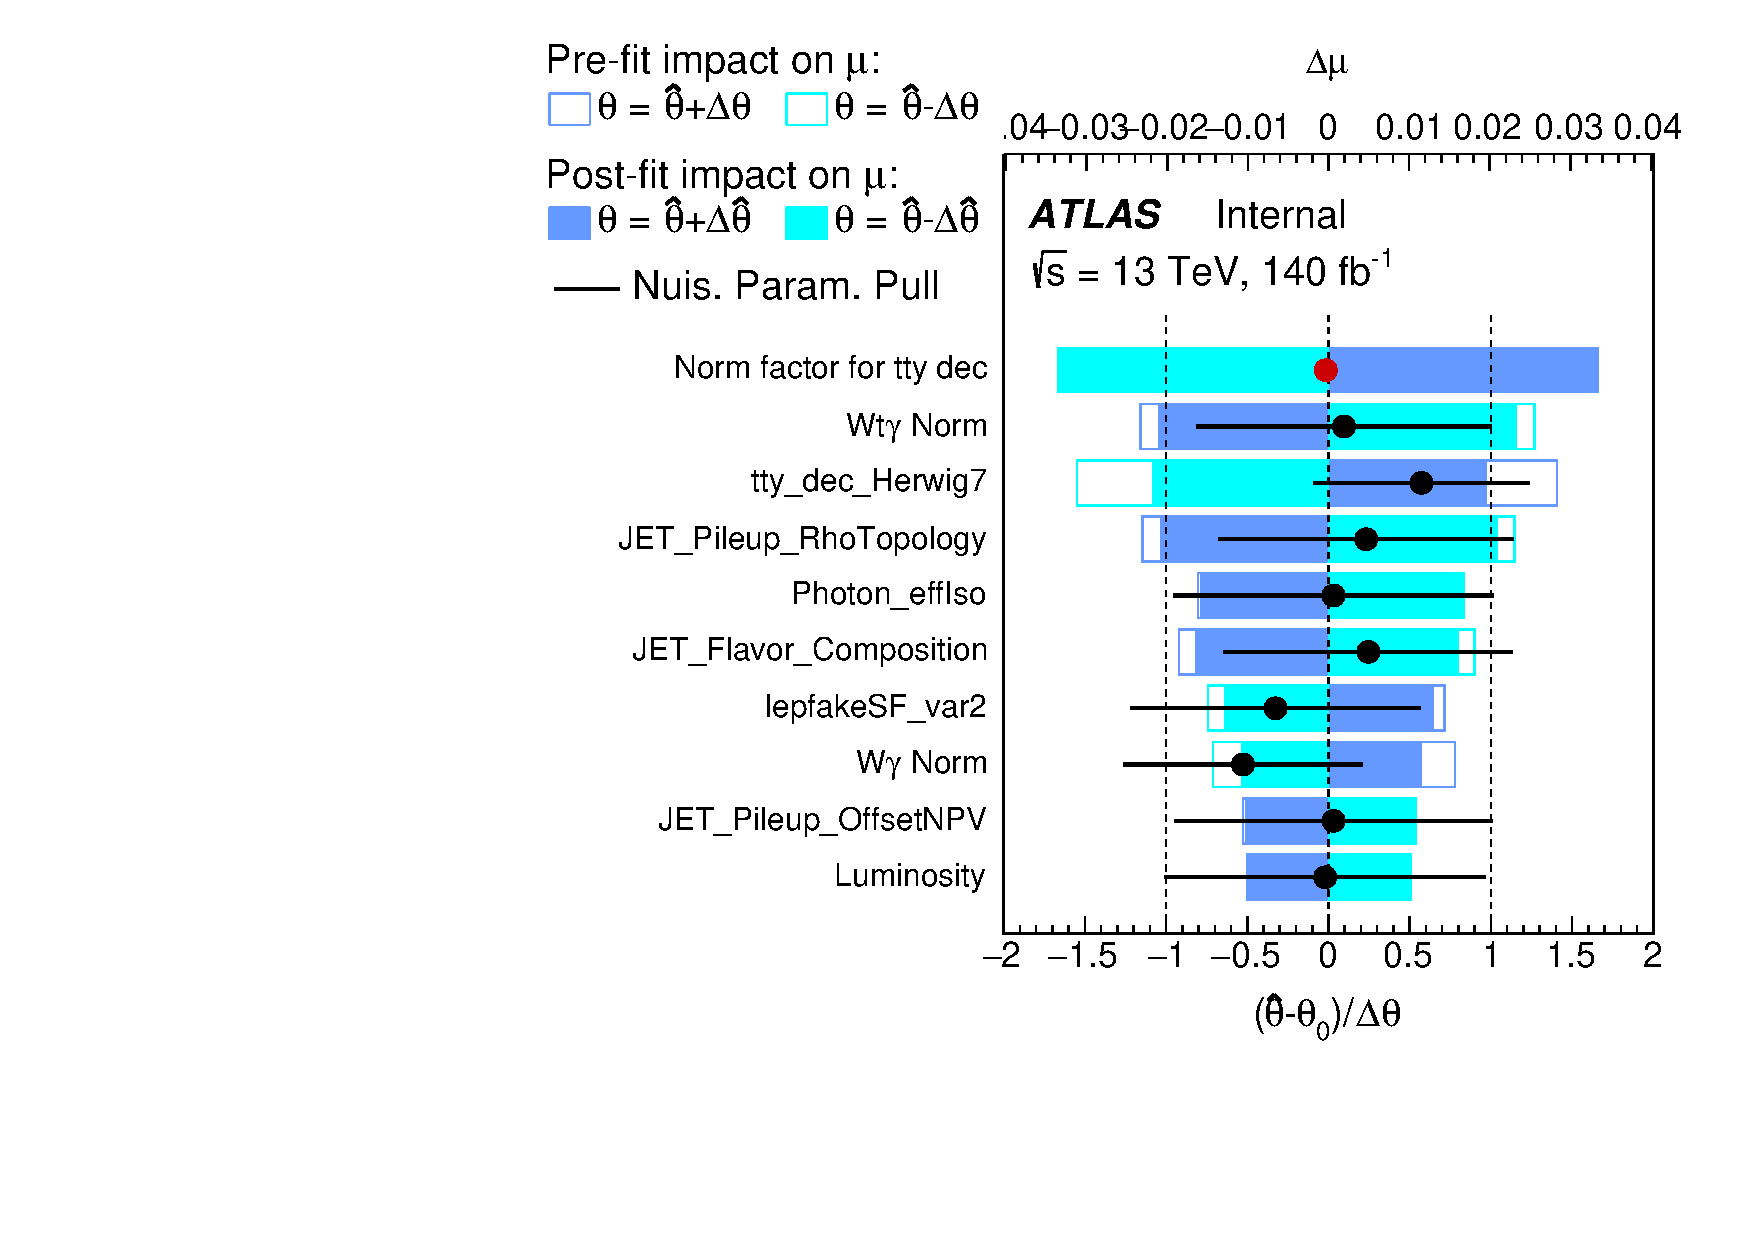
\includegraphics[width=0.2\textwidth]{figures/diff_xsec/ljet_dilep_combination_mu_blinded/Ranking/Ranking_tty_pt_Bin_005_mu.pdf}}
  \quad \quad
  \subfloat[]{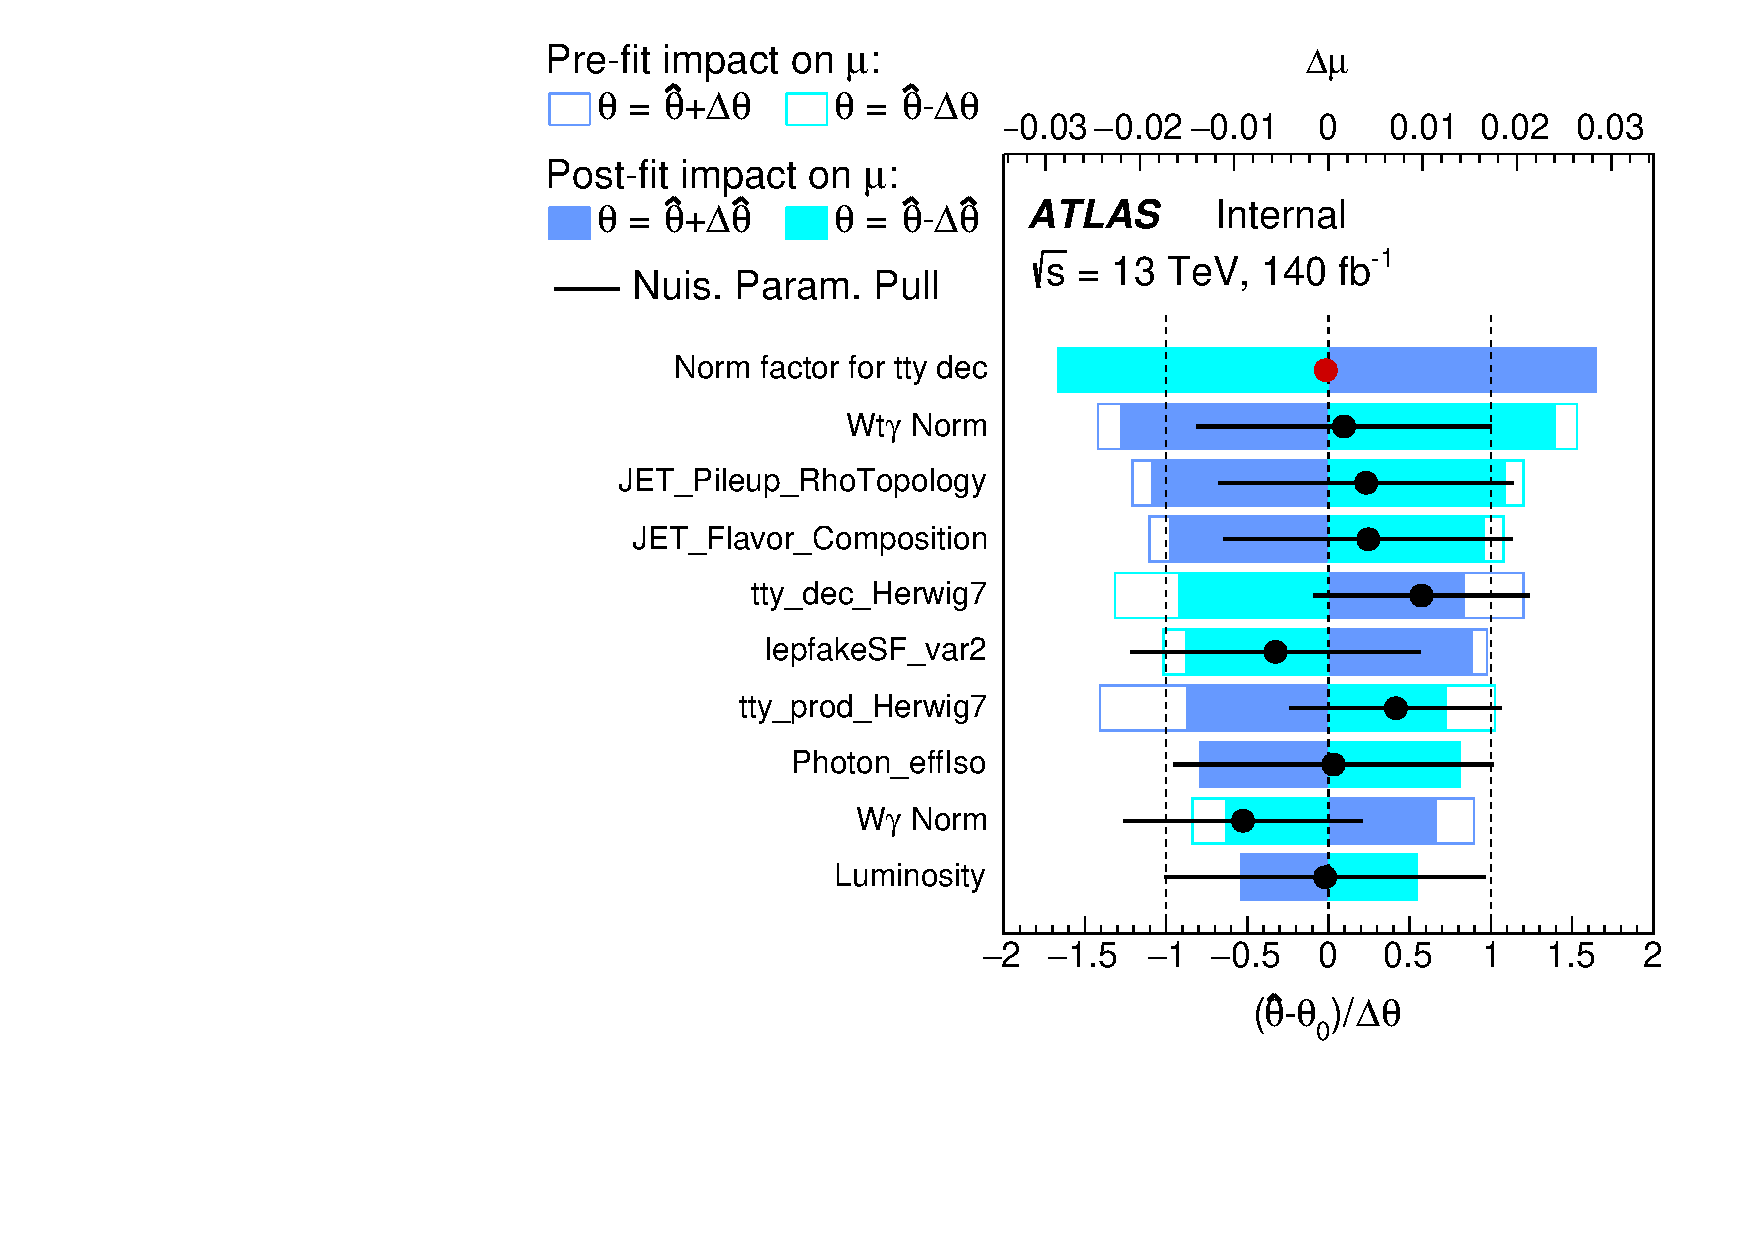
\includegraphics[width=0.2\textwidth]{figures/diff_xsec/ljet_dilep_combination_mu_blinded/Ranking/Ranking_tty_pt_Bin_006_mu.pdf}}
  \quad \quad
  \subfloat[]{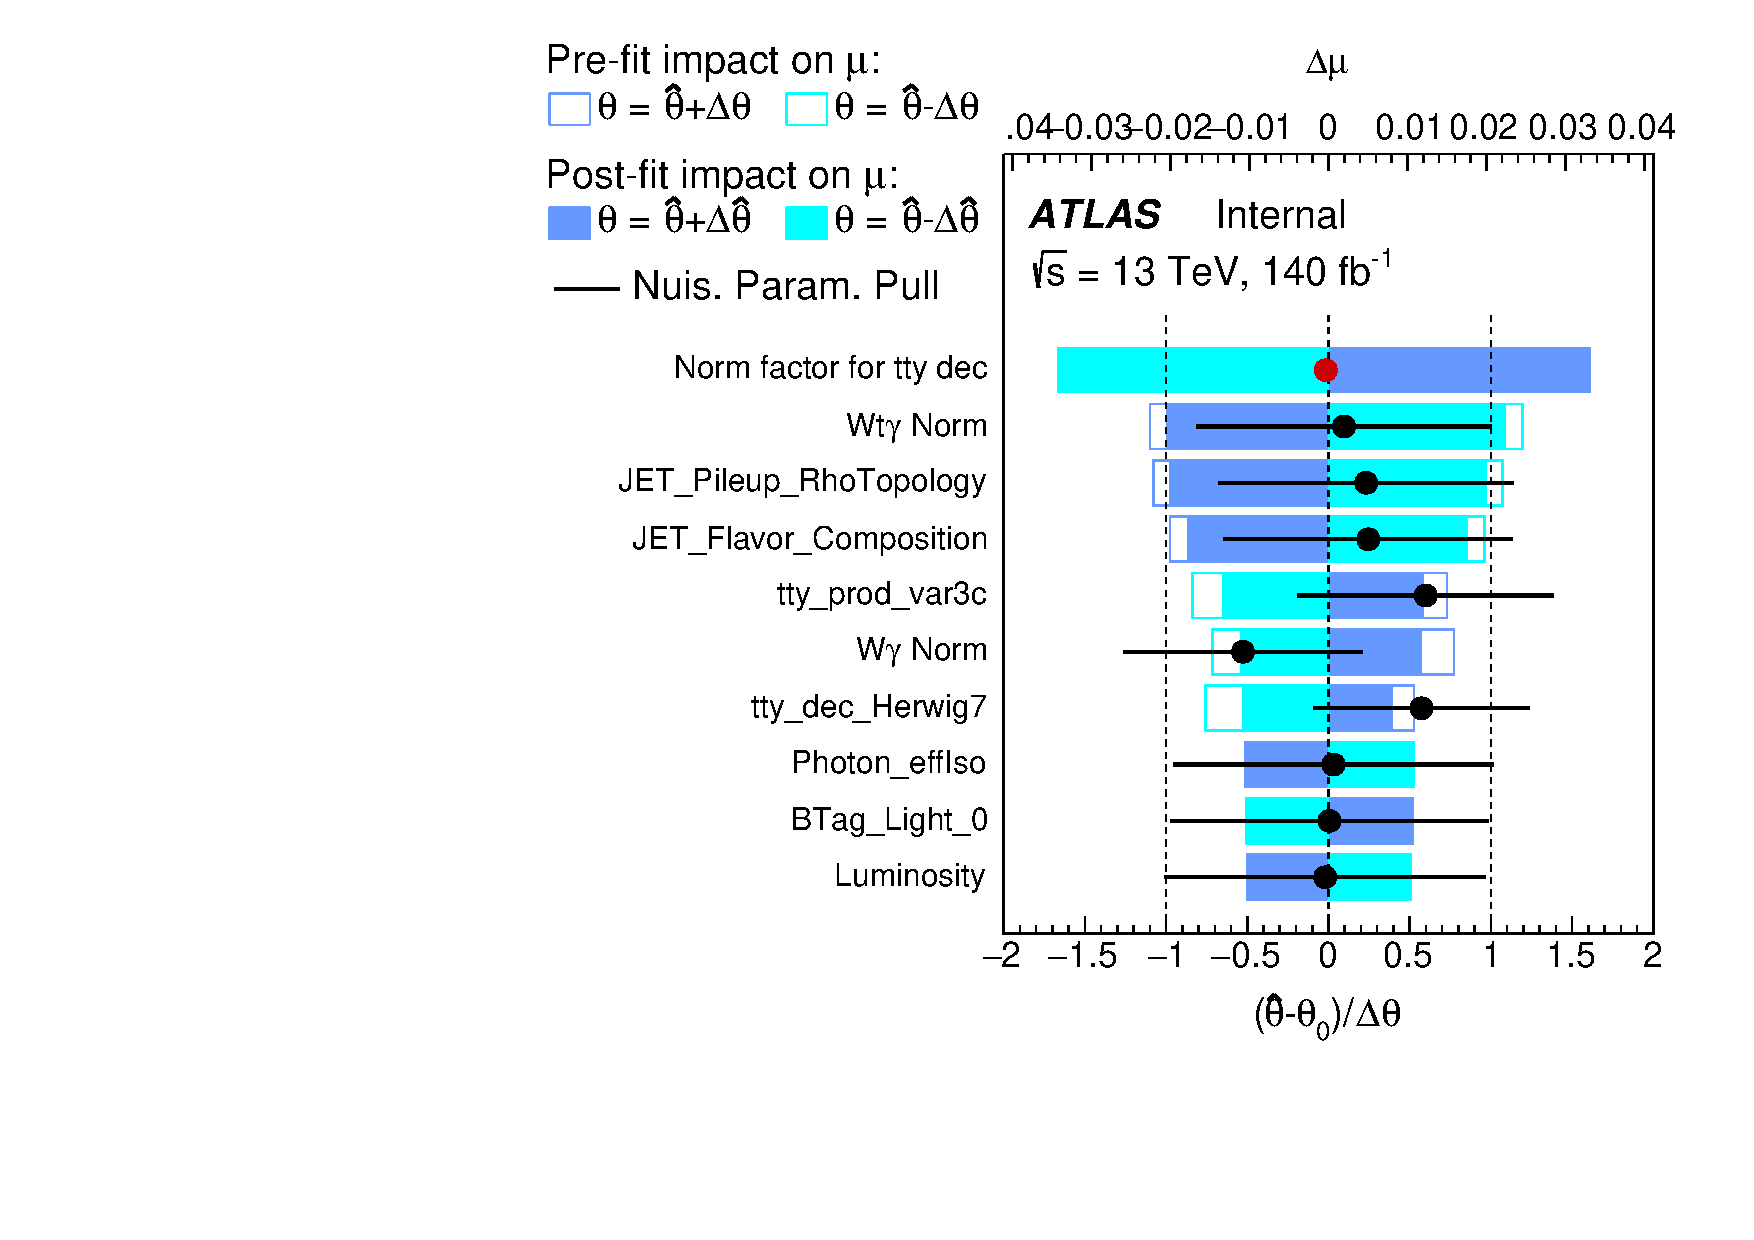
\includegraphics[width=0.2\textwidth]{figures/diff_xsec/ljet_dilep_combination_mu_blinded/Ranking/Ranking_tty_pt_Bin_007_mu.pdf}}
  \quad \quad
  \subfloat[]{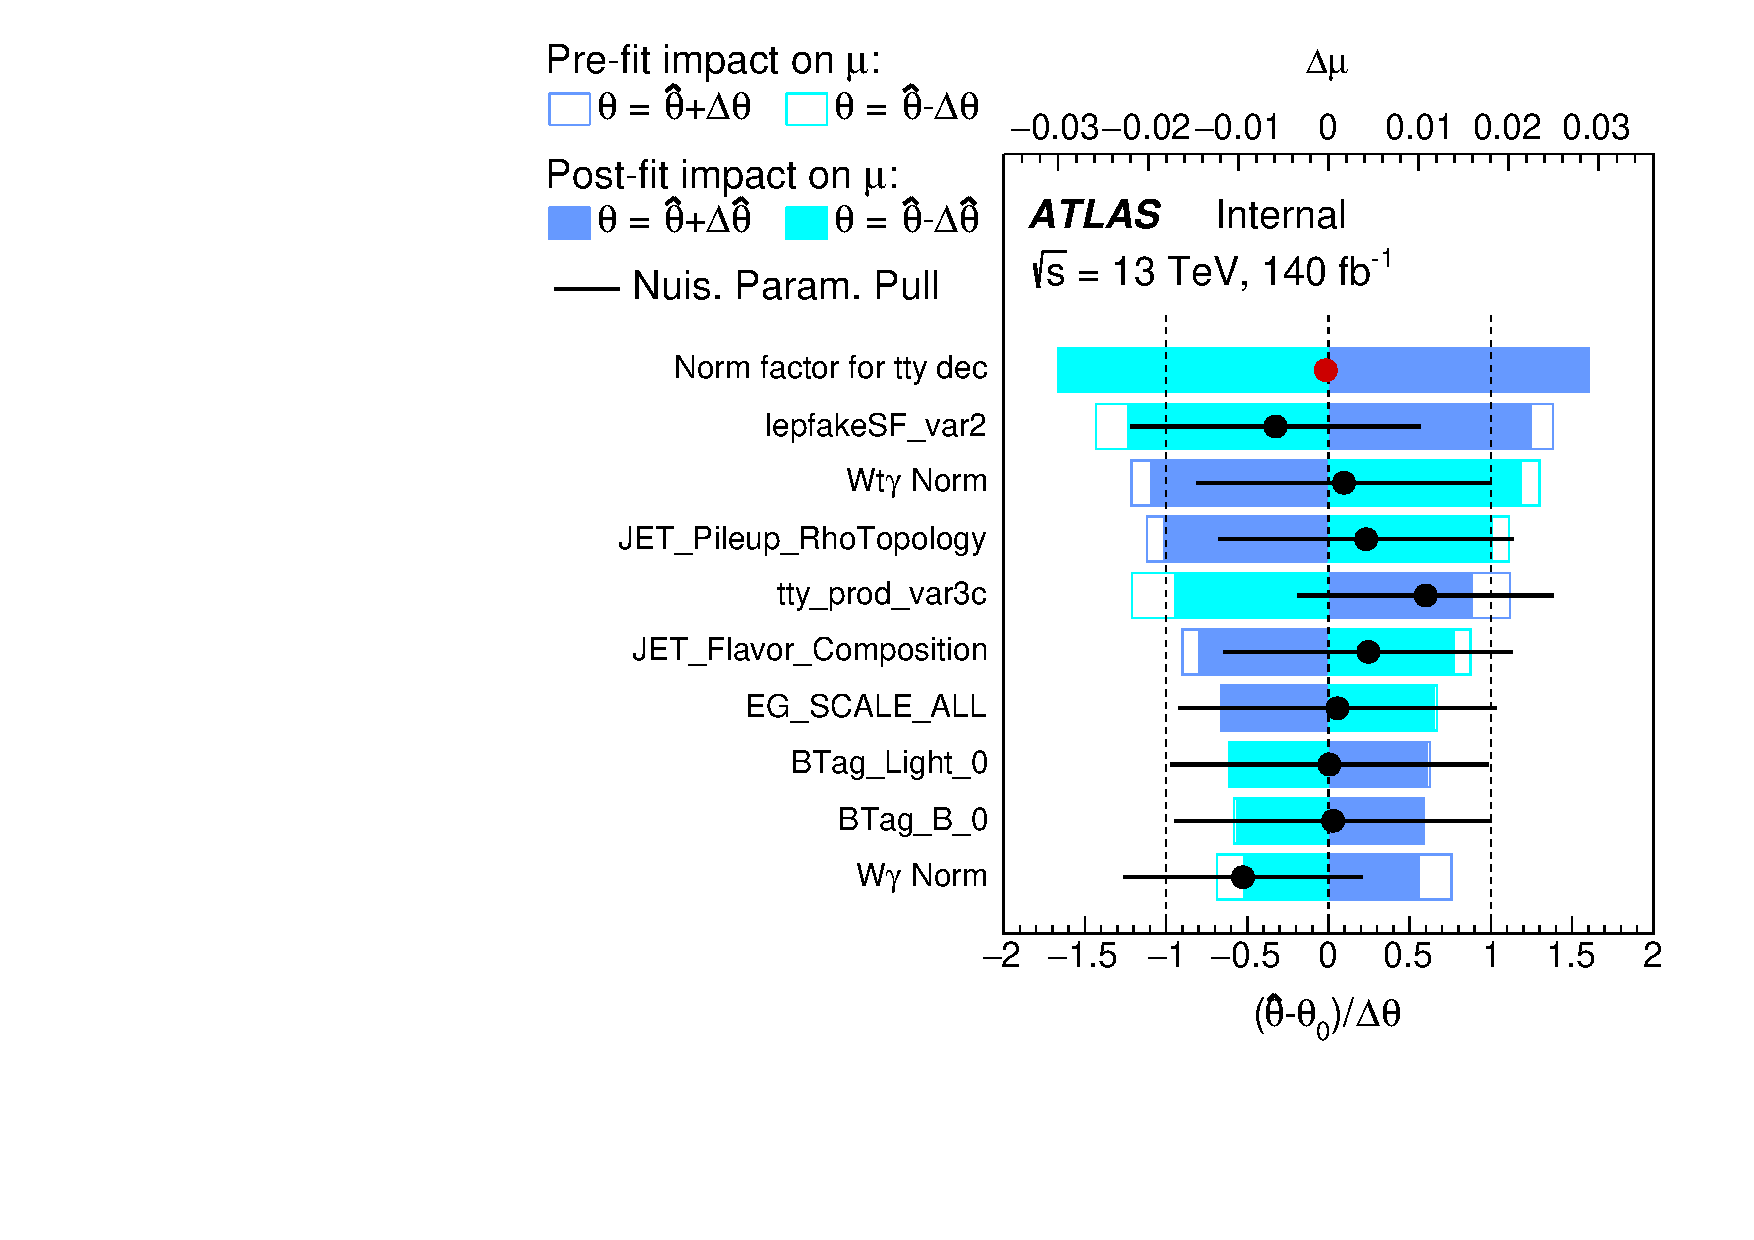
\includegraphics[width=0.2\textwidth]{figures/diff_xsec/ljet_dilep_combination_mu_blinded/Ranking/Ranking_tty_pt_Bin_008_mu.pdf}}
  \quad \quad
  \subfloat[]{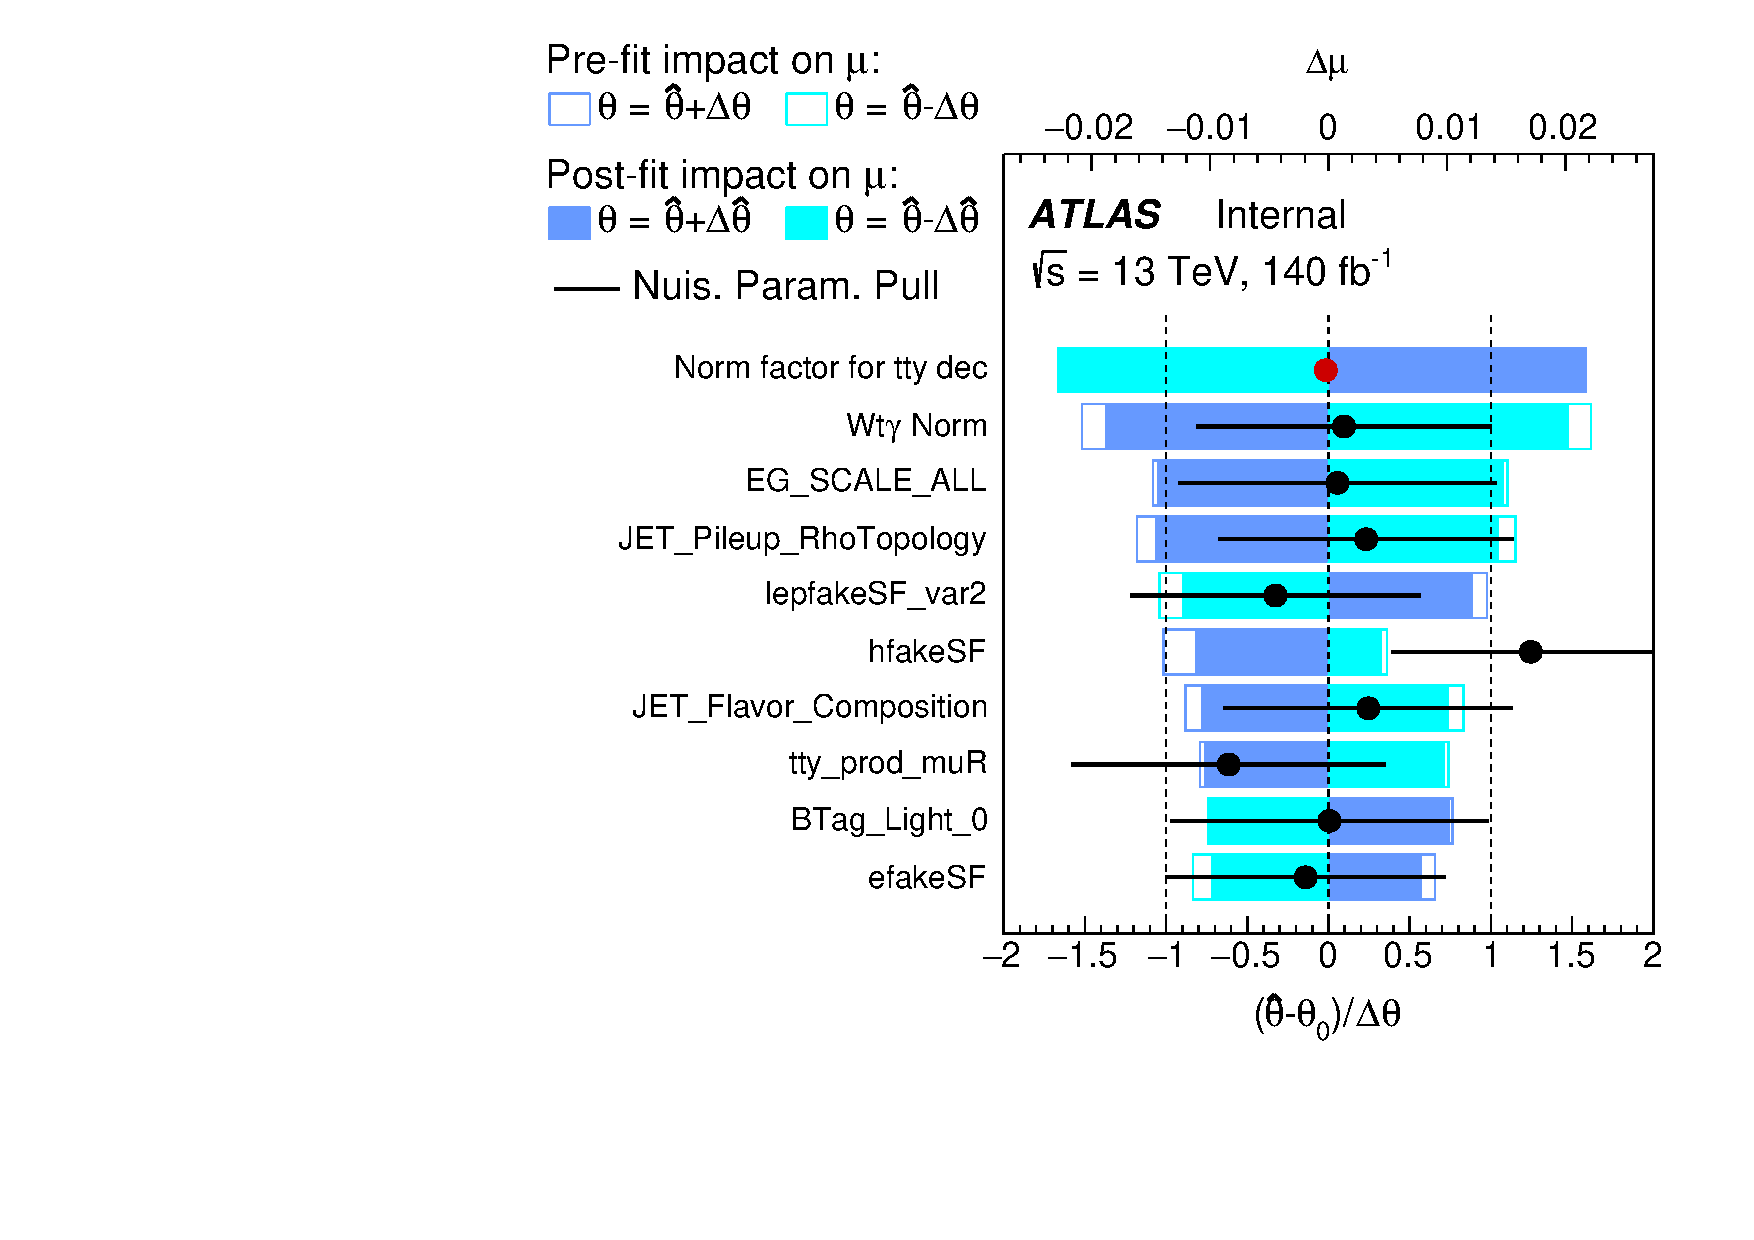
\includegraphics[width=0.2\textwidth]{figures/diff_xsec/ljet_dilep_combination_mu_blinded/Ranking/Ranking_tty_pt_Bin_009_mu.pdf}}
  \quad \quad
  \subfloat[]{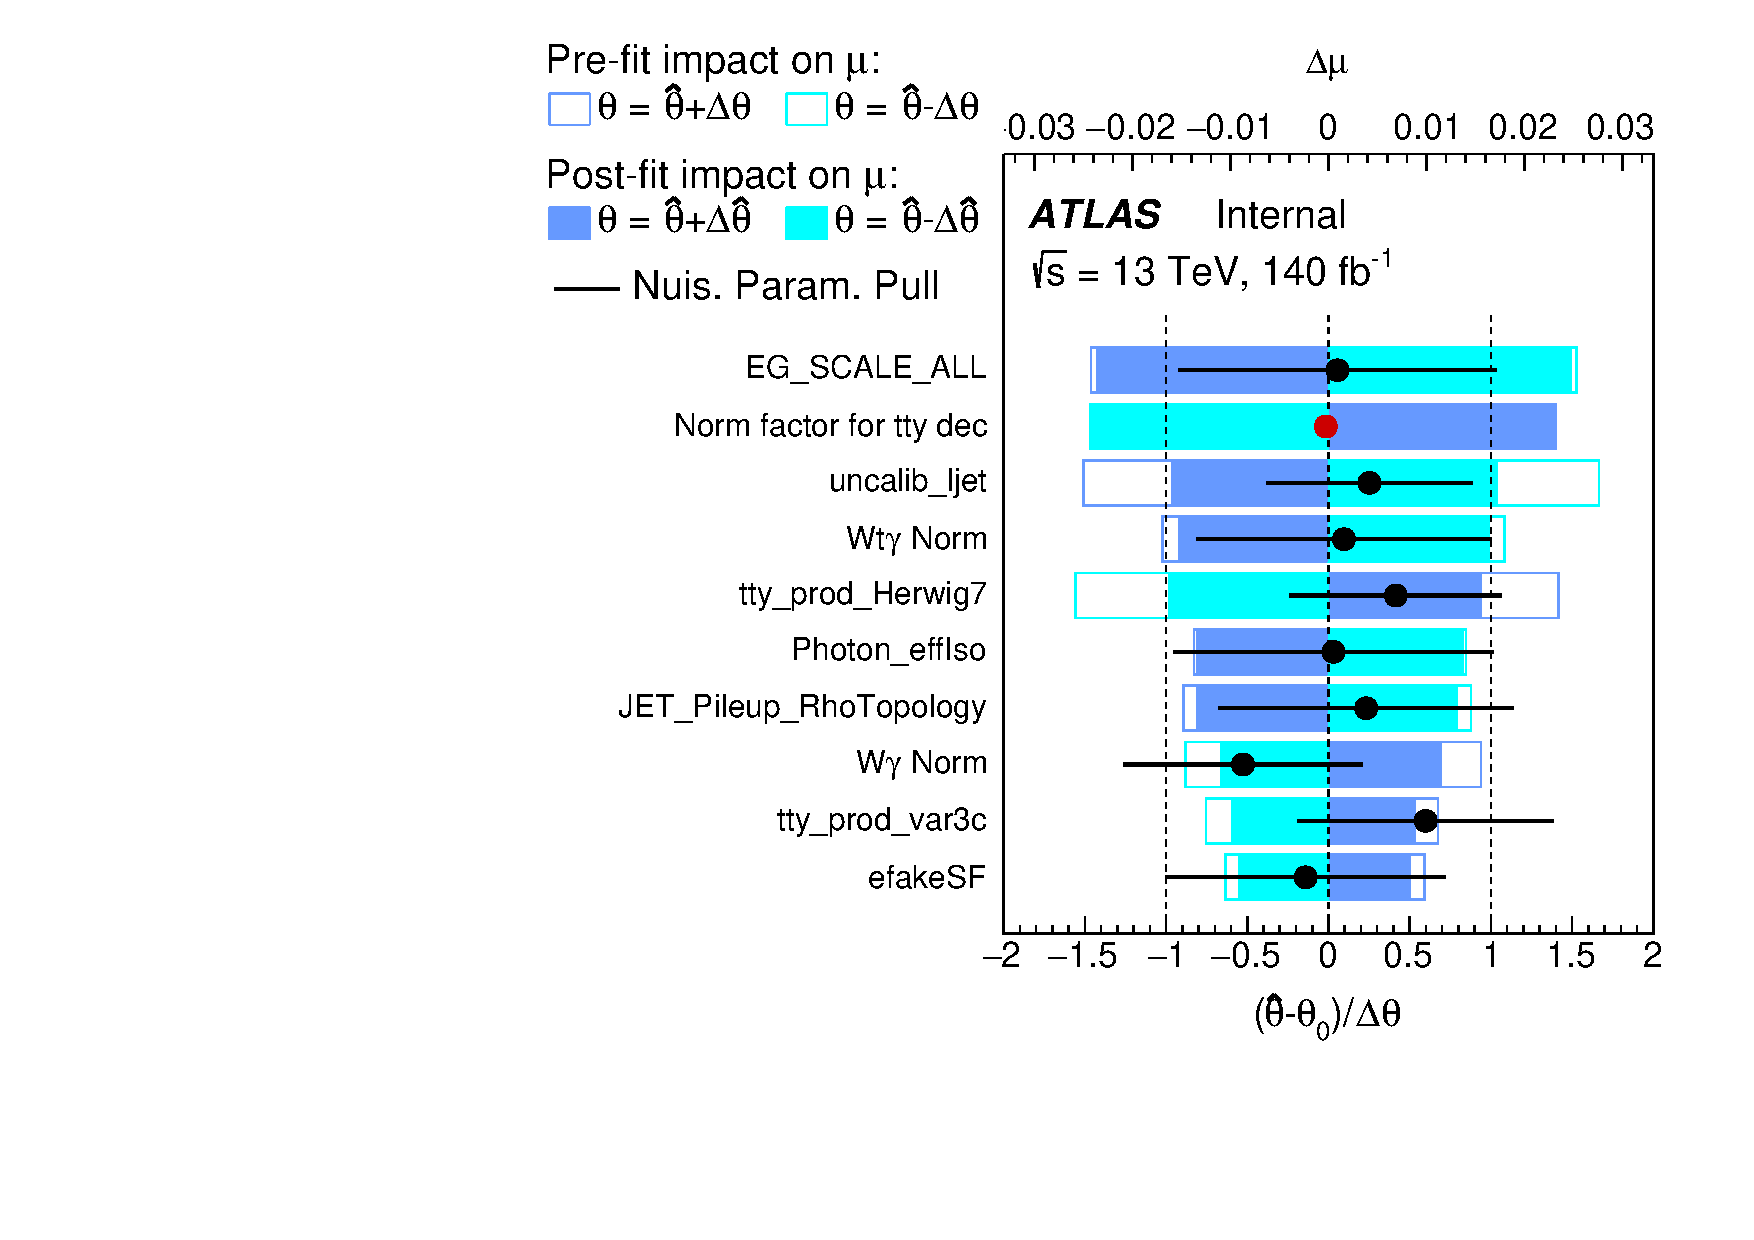
\includegraphics[width=0.2\textwidth]{figures/diff_xsec/ljet_dilep_combination_mu_blinded/Ranking/Ranking_tty_pt_Bin_010_mu.pdf}}

  \caption{Ranking plots of the 10 NPs with the largest impact on the \tty production singal strength in each bin of the $p_T(\gamma)$ distribution in the combined single 
  lepton and dilepton channel. Each subfigure, labeled (a), (b), (c), (d)... (j), corresponds to a specific bin 
  of the $p_T(\gamma)$ distribution, with bin 1 represented in subfigure (a), bin 2 represented in 
  subfigure (b), and so on.}
  \label{fig:ranking_sldl_tty_prod_mu_blinded}
\end{figure}
\FloatBarrier

%%%%%%%%%%%% UNFOLDED Distributions %%%%%%%%%%%%%%%%%%%%%
\begin{figure}[ht]
  \centering
  \subfloat[]{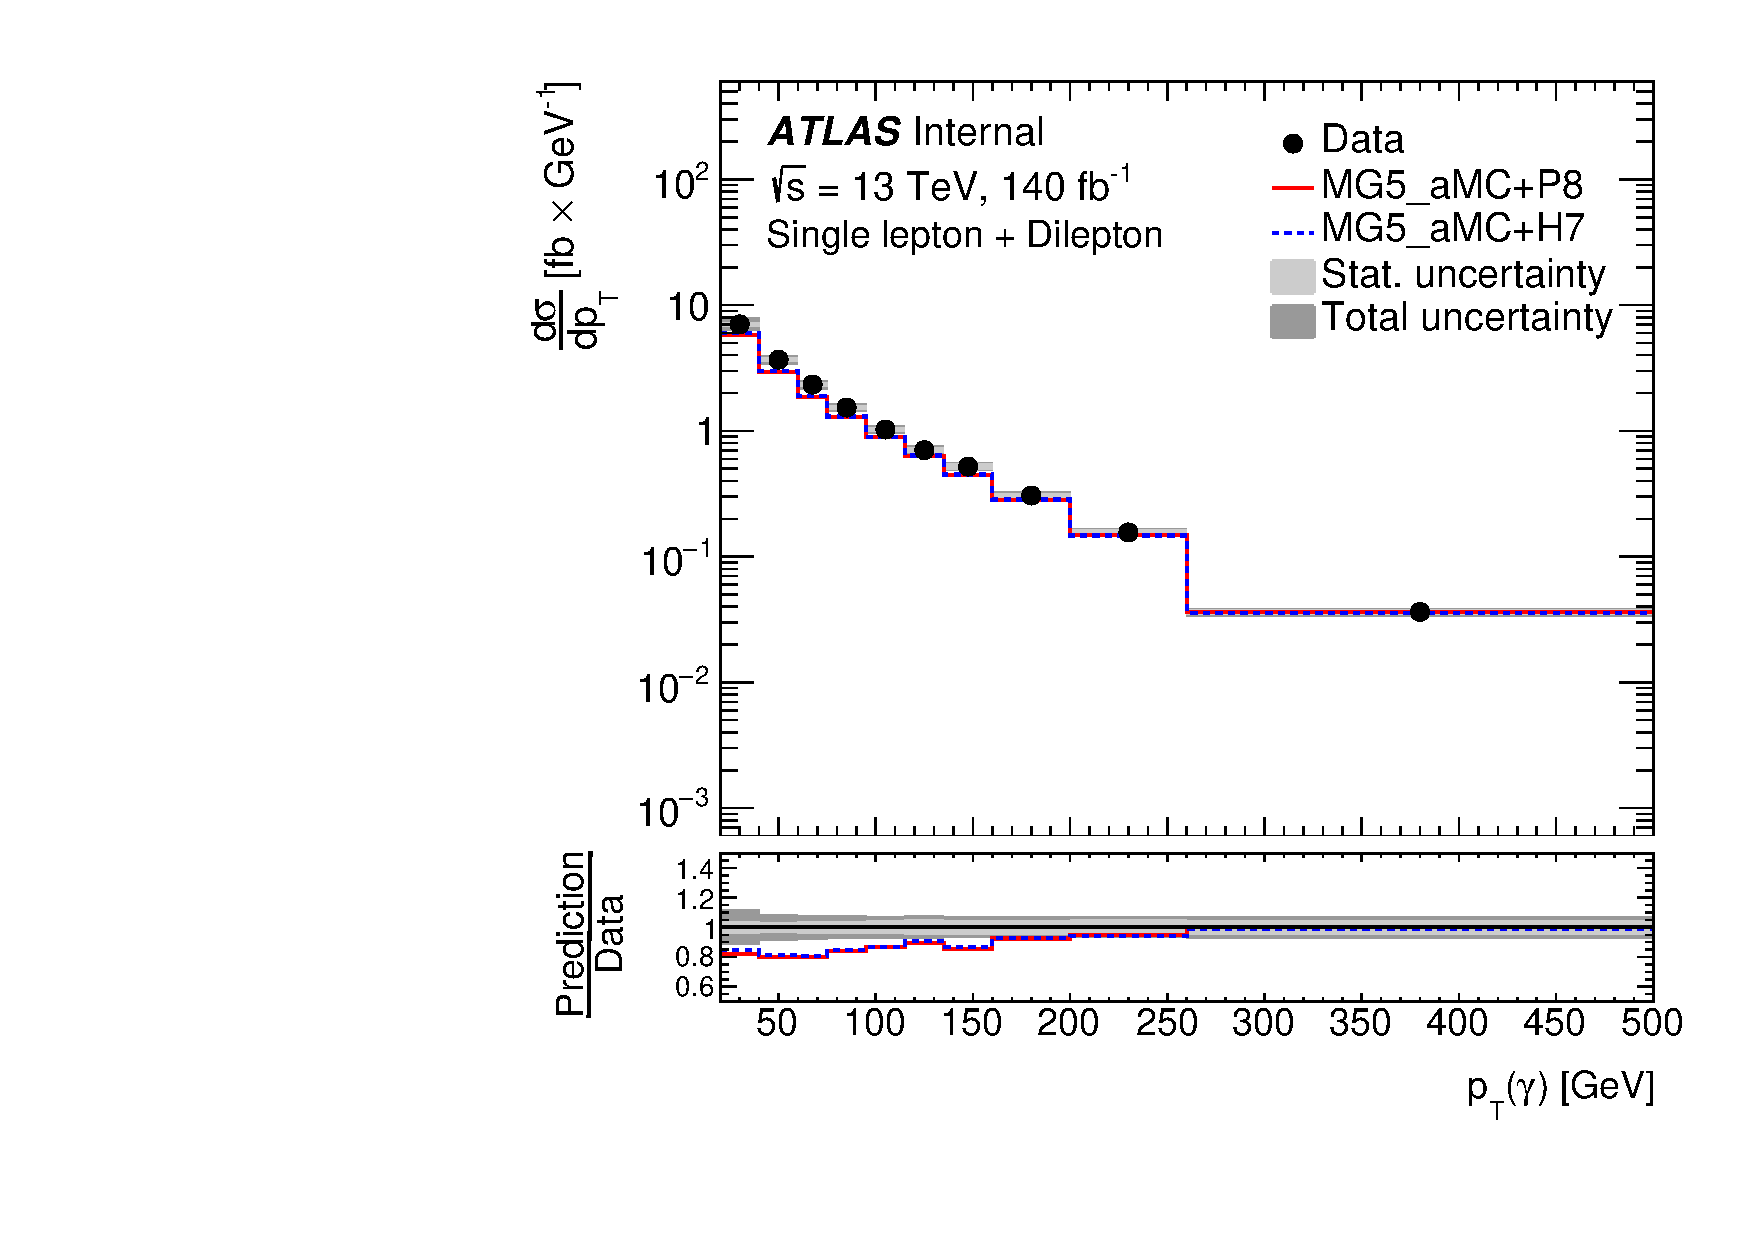
\includegraphics[width=0.4\textwidth]{figures/diff_xsec/absolute-unfolded-distributions/tty_prod_SLDL/tty_pt_UnfoldedData.pdf}}
  \quad\quad
  \subfloat[]{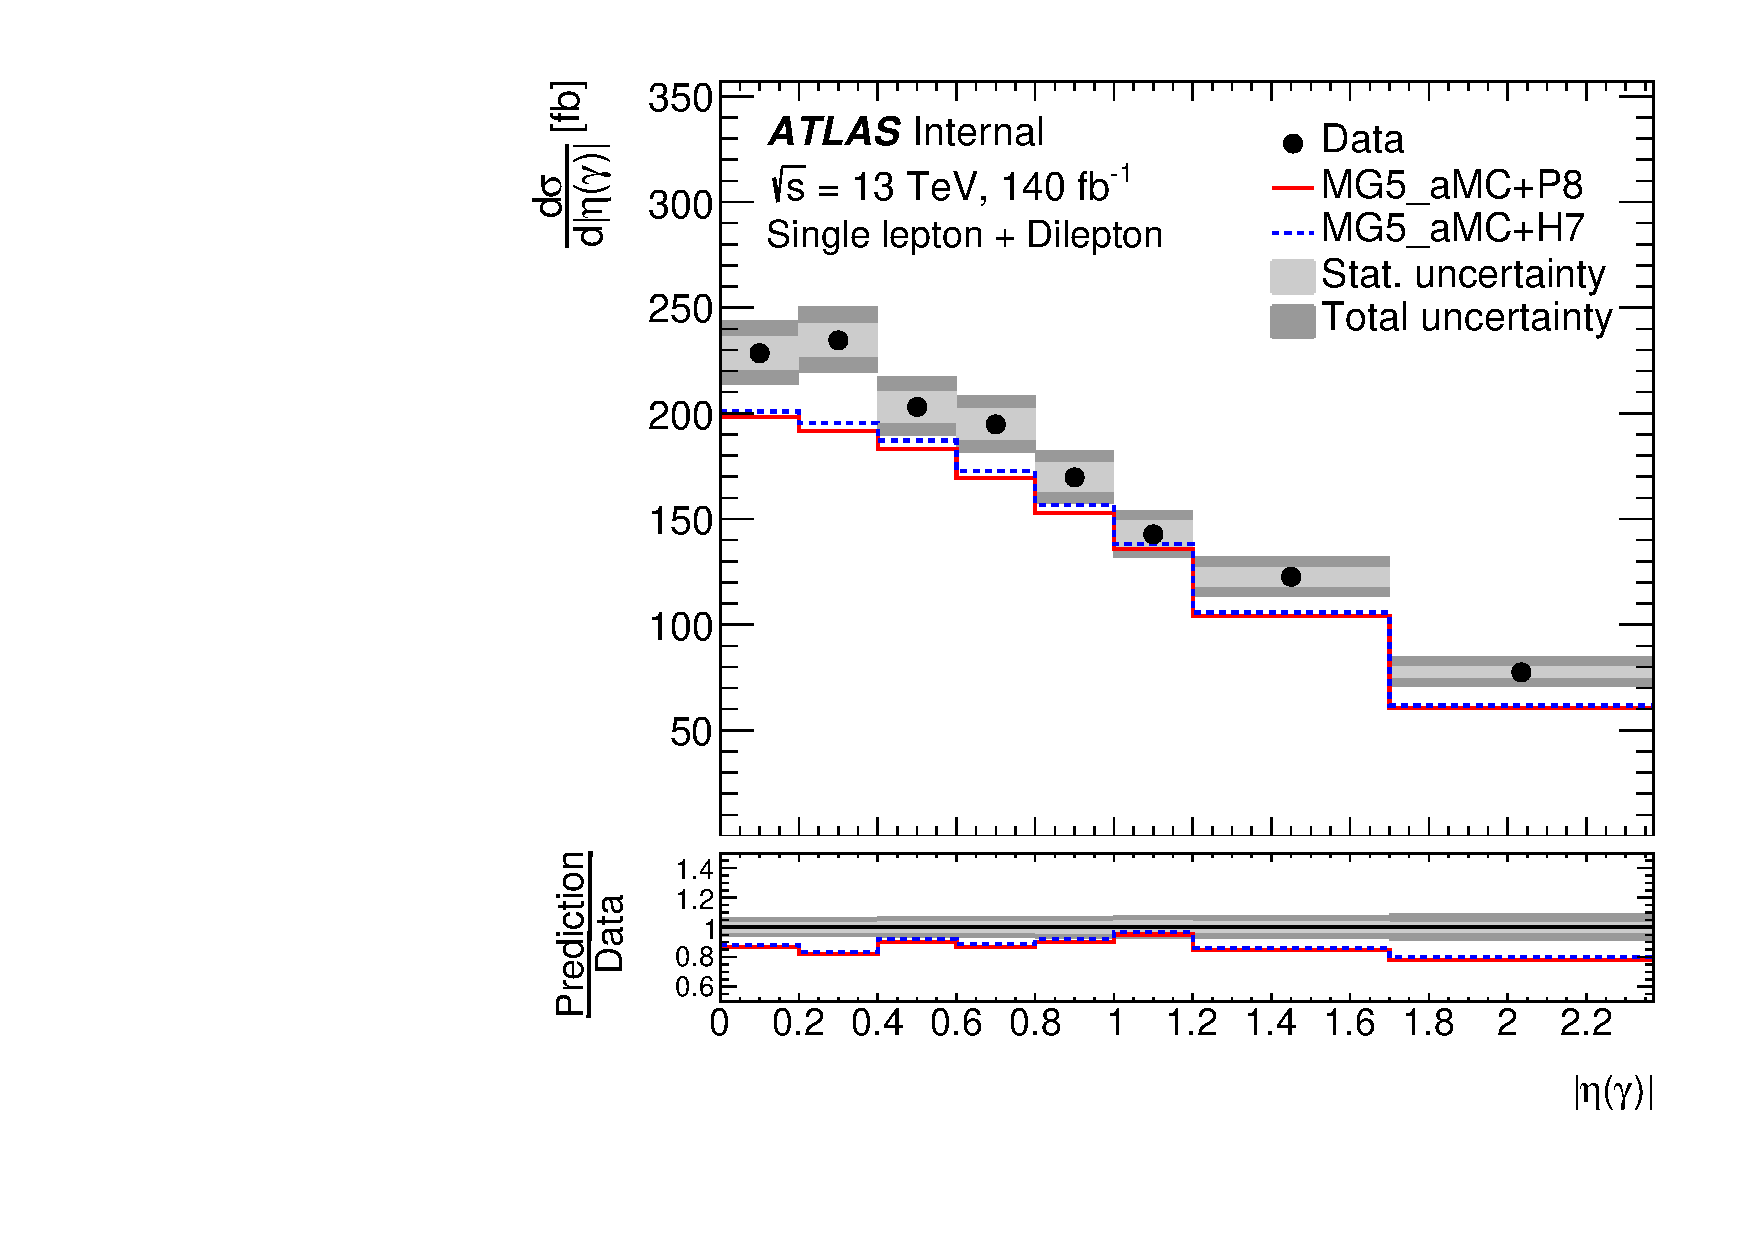
\includegraphics[width=0.4\textwidth]{figures/diff_xsec/absolute-unfolded-distributions/tty_prod_SLDL/tty_eta_UnfoldedData.pdf}}
  \caption{For the $t\bar{t}\gamma(\mathrm{production})$ measurement, particle-level unfolded distributions in the combined single lepton and dilepton channel after fitting to the real dataset. 
  The error bars represent both statistical and systematic uncertainties. (a) $p_T(\gamma)$, (b) $|\eta(\gamma|)$. Overflow events are included in the last bin of the corresponding distribution.}
  \label{fig:pt_unfolded_dist_sldl_tty_prod_realdata}
\end{figure}
\FloatBarrier


%%%%%%%%%%%%%%%%%%%%%%%%%%%%%%%%%%%%%%%%%%%%%%%%%%%%%%%%%%%%%%%%%%%%%%%%%%%%%%%%
%%%%%%%%%%%%%%  Normalized distributions %%%%%%%%%%%%%%%%%%%%%%%%%%%%%%%%%%%%%%%
%%%%%%%%%%%%%%%%%%%%%%%%%%%%%%%%%%%%%%%%%%%%%%%%%%%%%%%%%%%%%%%%%%%%%%%%%%%%%%%%


\begin{figure}[ht]
  \centering
  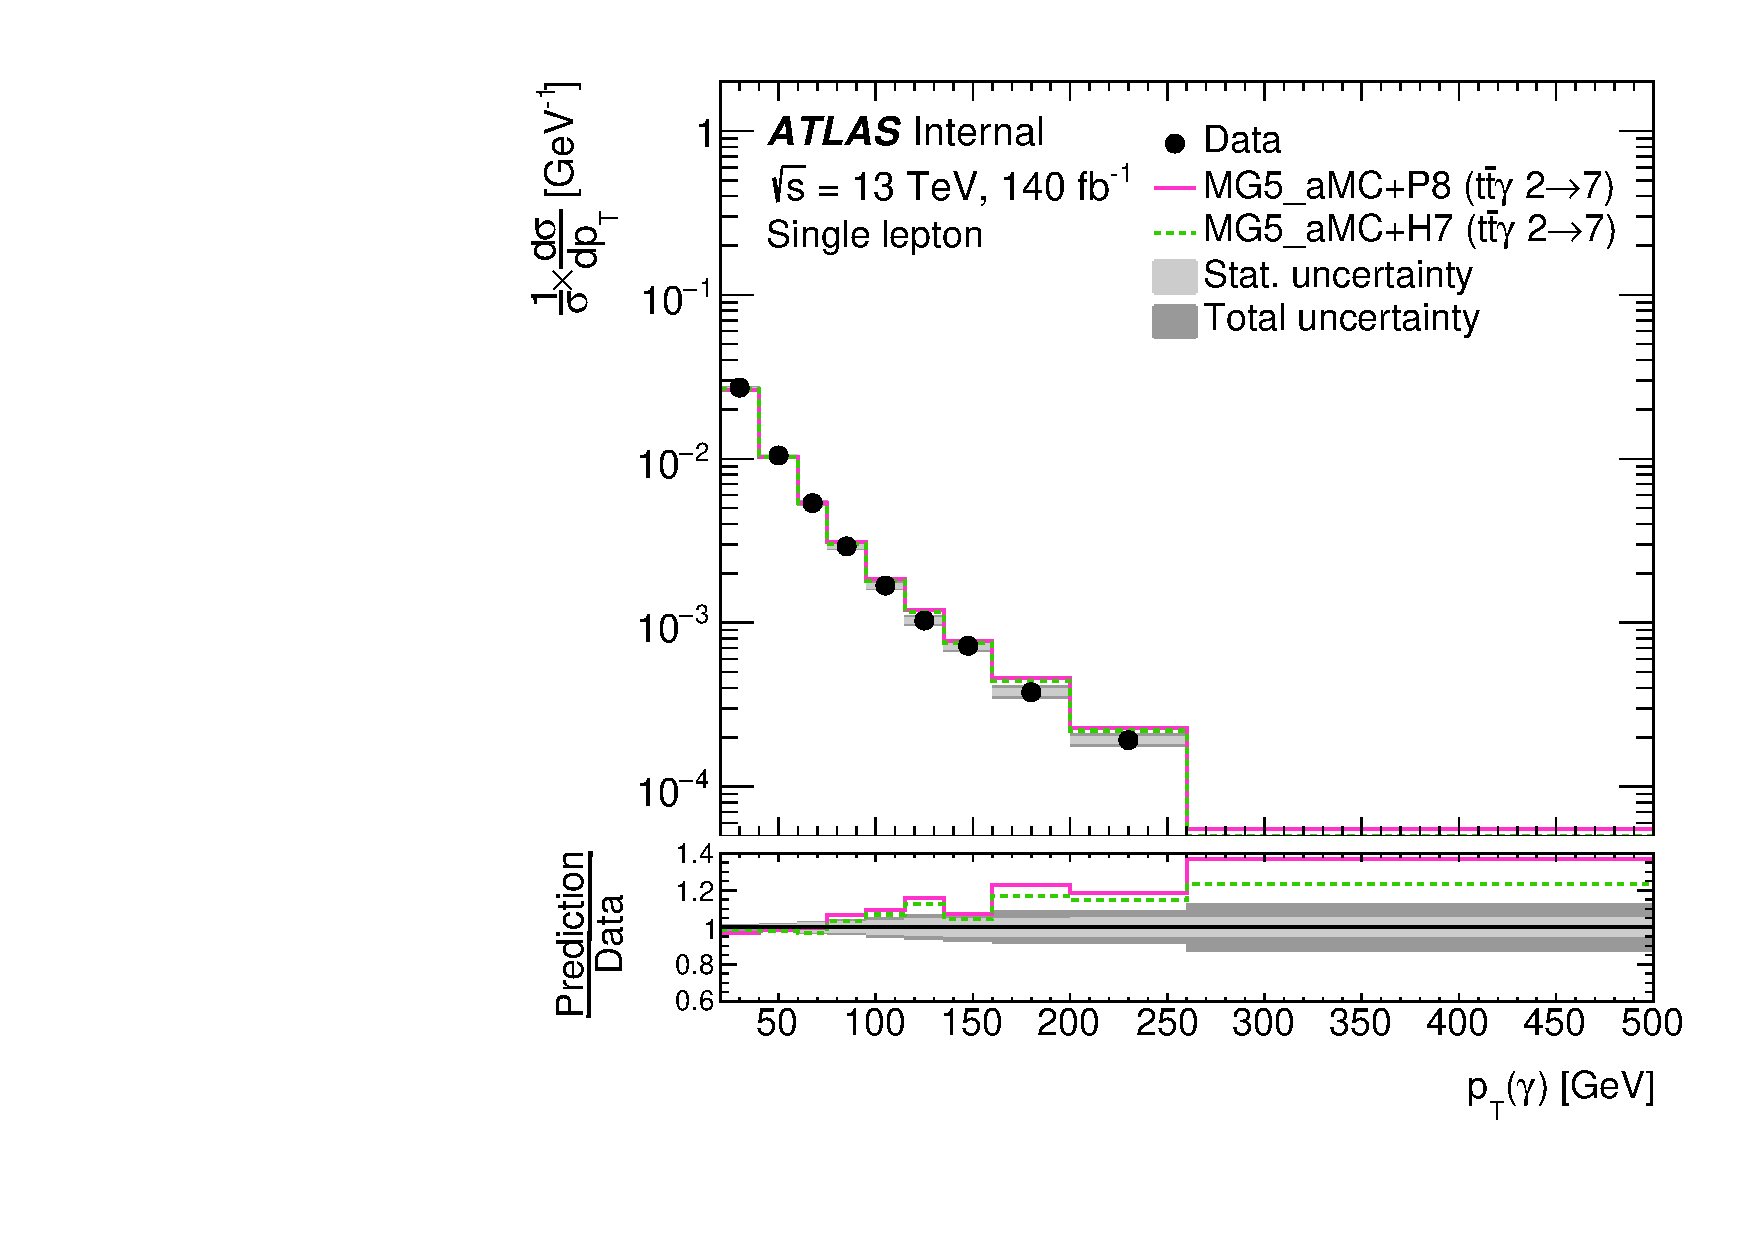
\includegraphics[width=0.33\textwidth]{figures/diff_xsec/normalized-unfolded-distributions/tty_total_ljet/SL_tty_total_pt_unfolded_normalized.pdf}%
  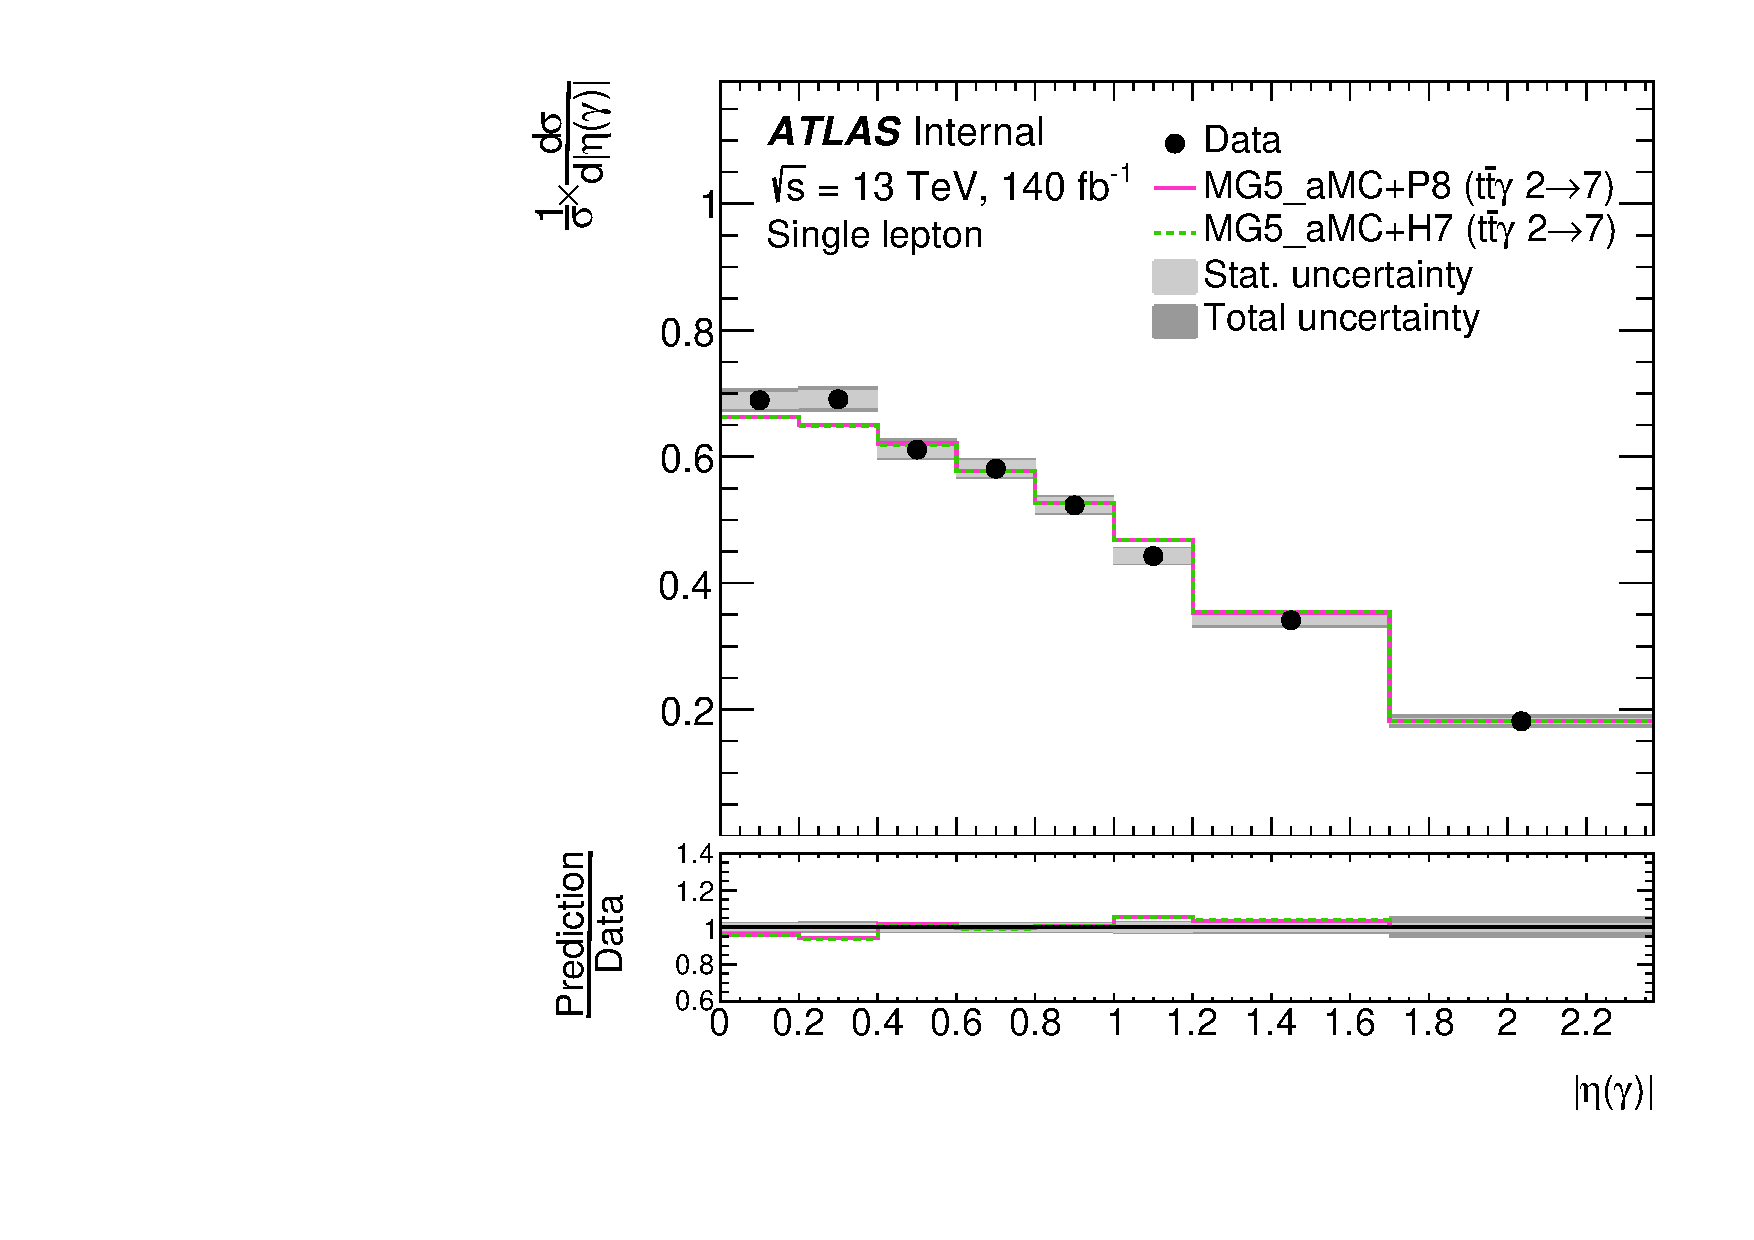
\includegraphics[width=0.33\textwidth]{figures/diff_xsec/normalized-unfolded-distributions/tty_total_ljet/SL_tty_total_eta_unfolded_normalized.pdf}%
  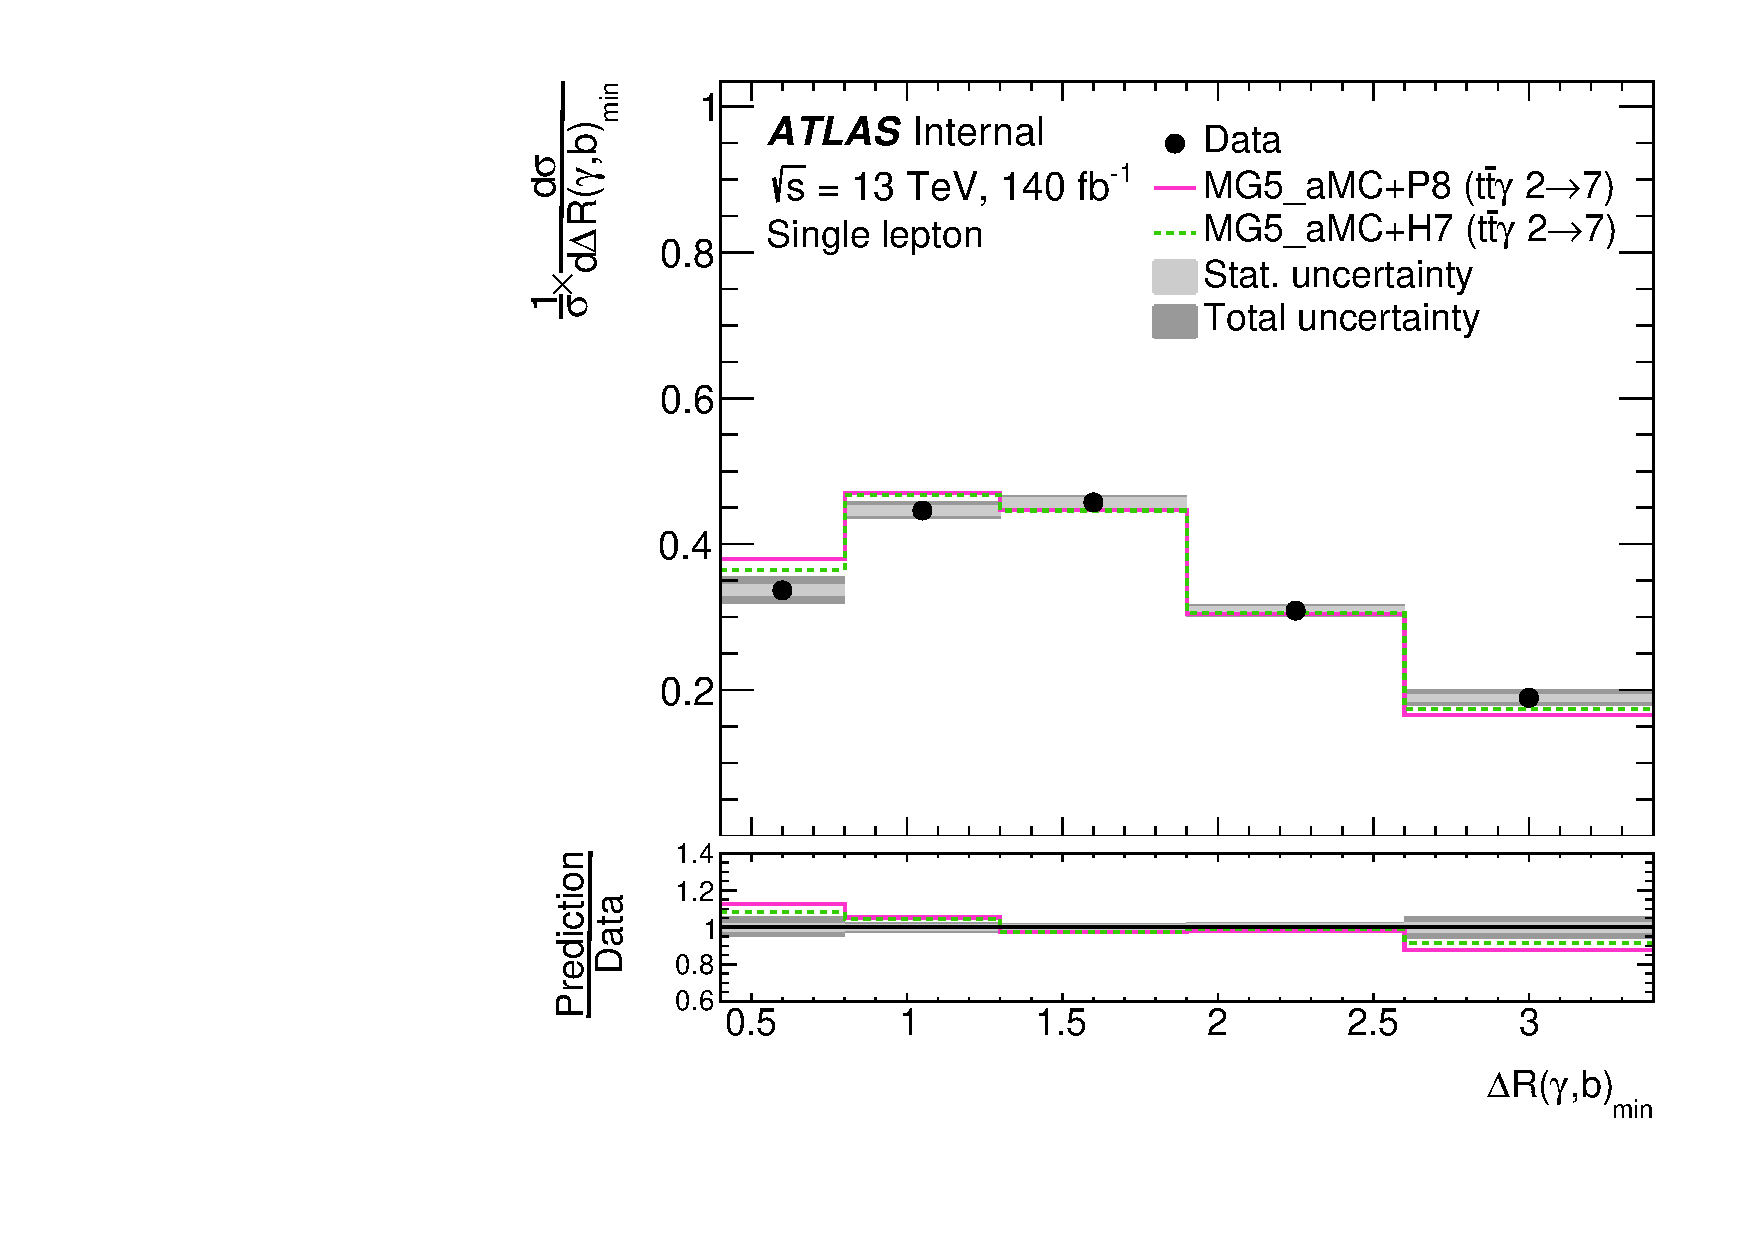
\includegraphics[width=0.33\textwidth]{figures/diff_xsec/normalized-unfolded-distributions/tty_total_ljet/SL_tty_total_drphb_unfolded_normalized.pdf}\\
  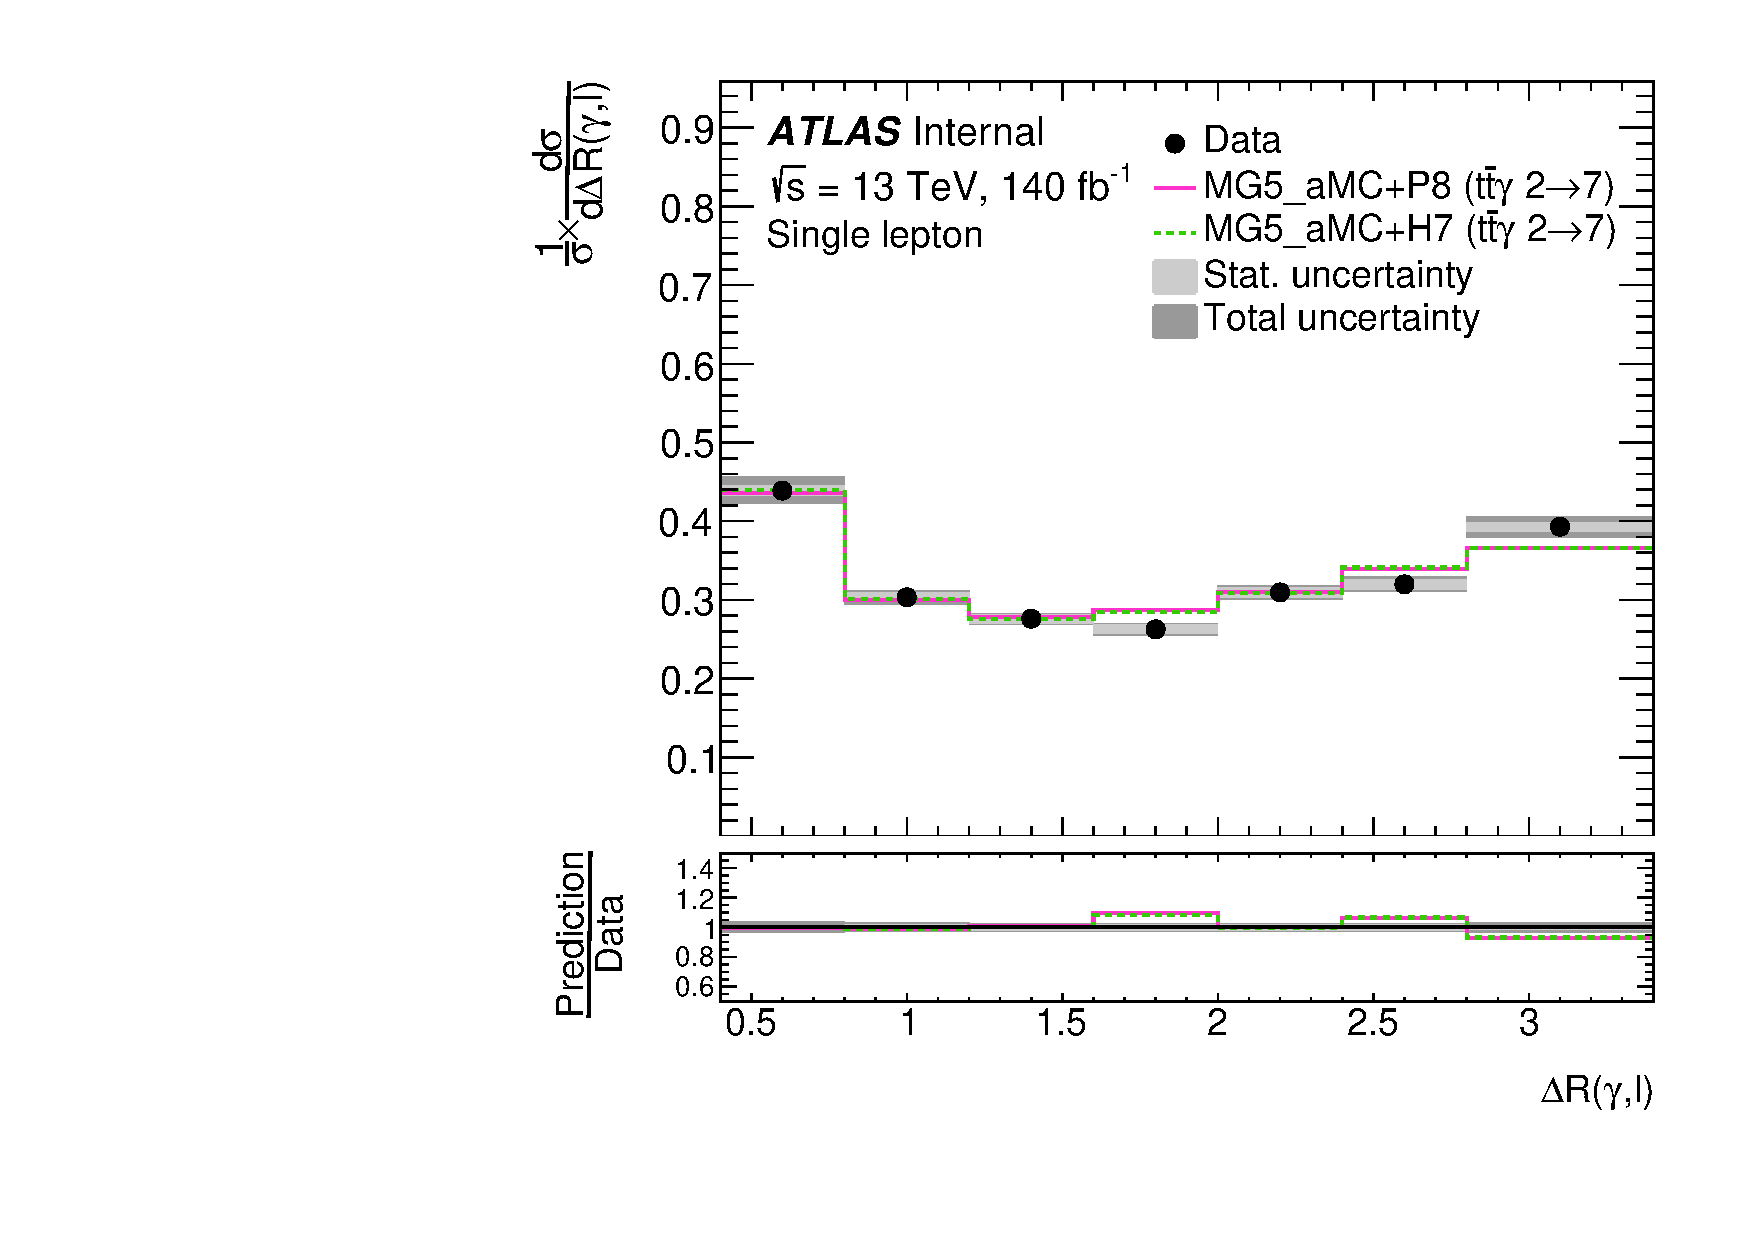
\includegraphics[width=0.33\textwidth]{figures/diff_xsec/normalized-unfolded-distributions/tty_total_ljet/SL_tty_total_drphl_unfolded_normalized.pdf}%
  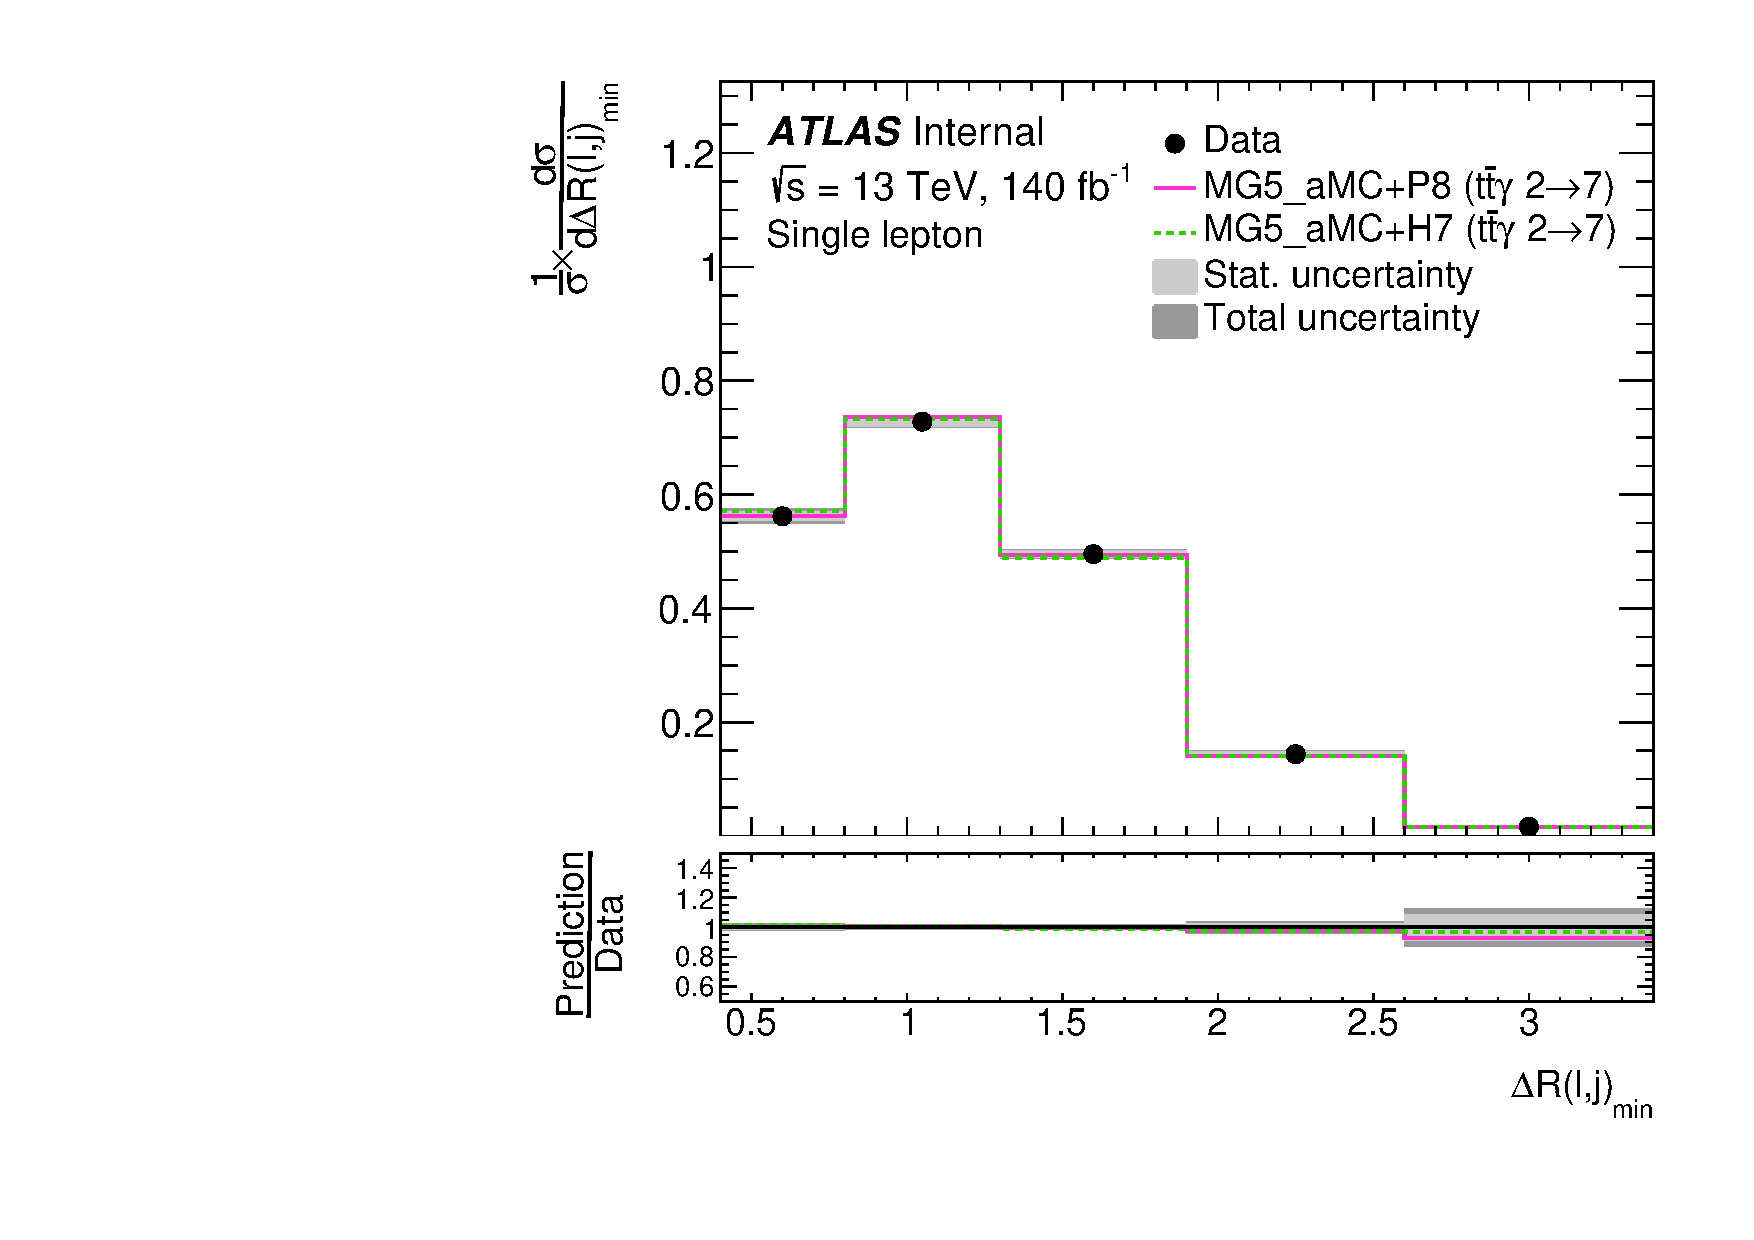
\includegraphics[width=0.33\textwidth]{figures/diff_xsec/normalized-unfolded-distributions/tty_total_ljet/SL_tty_total_drlj_unfolded_normalized.pdf}%
  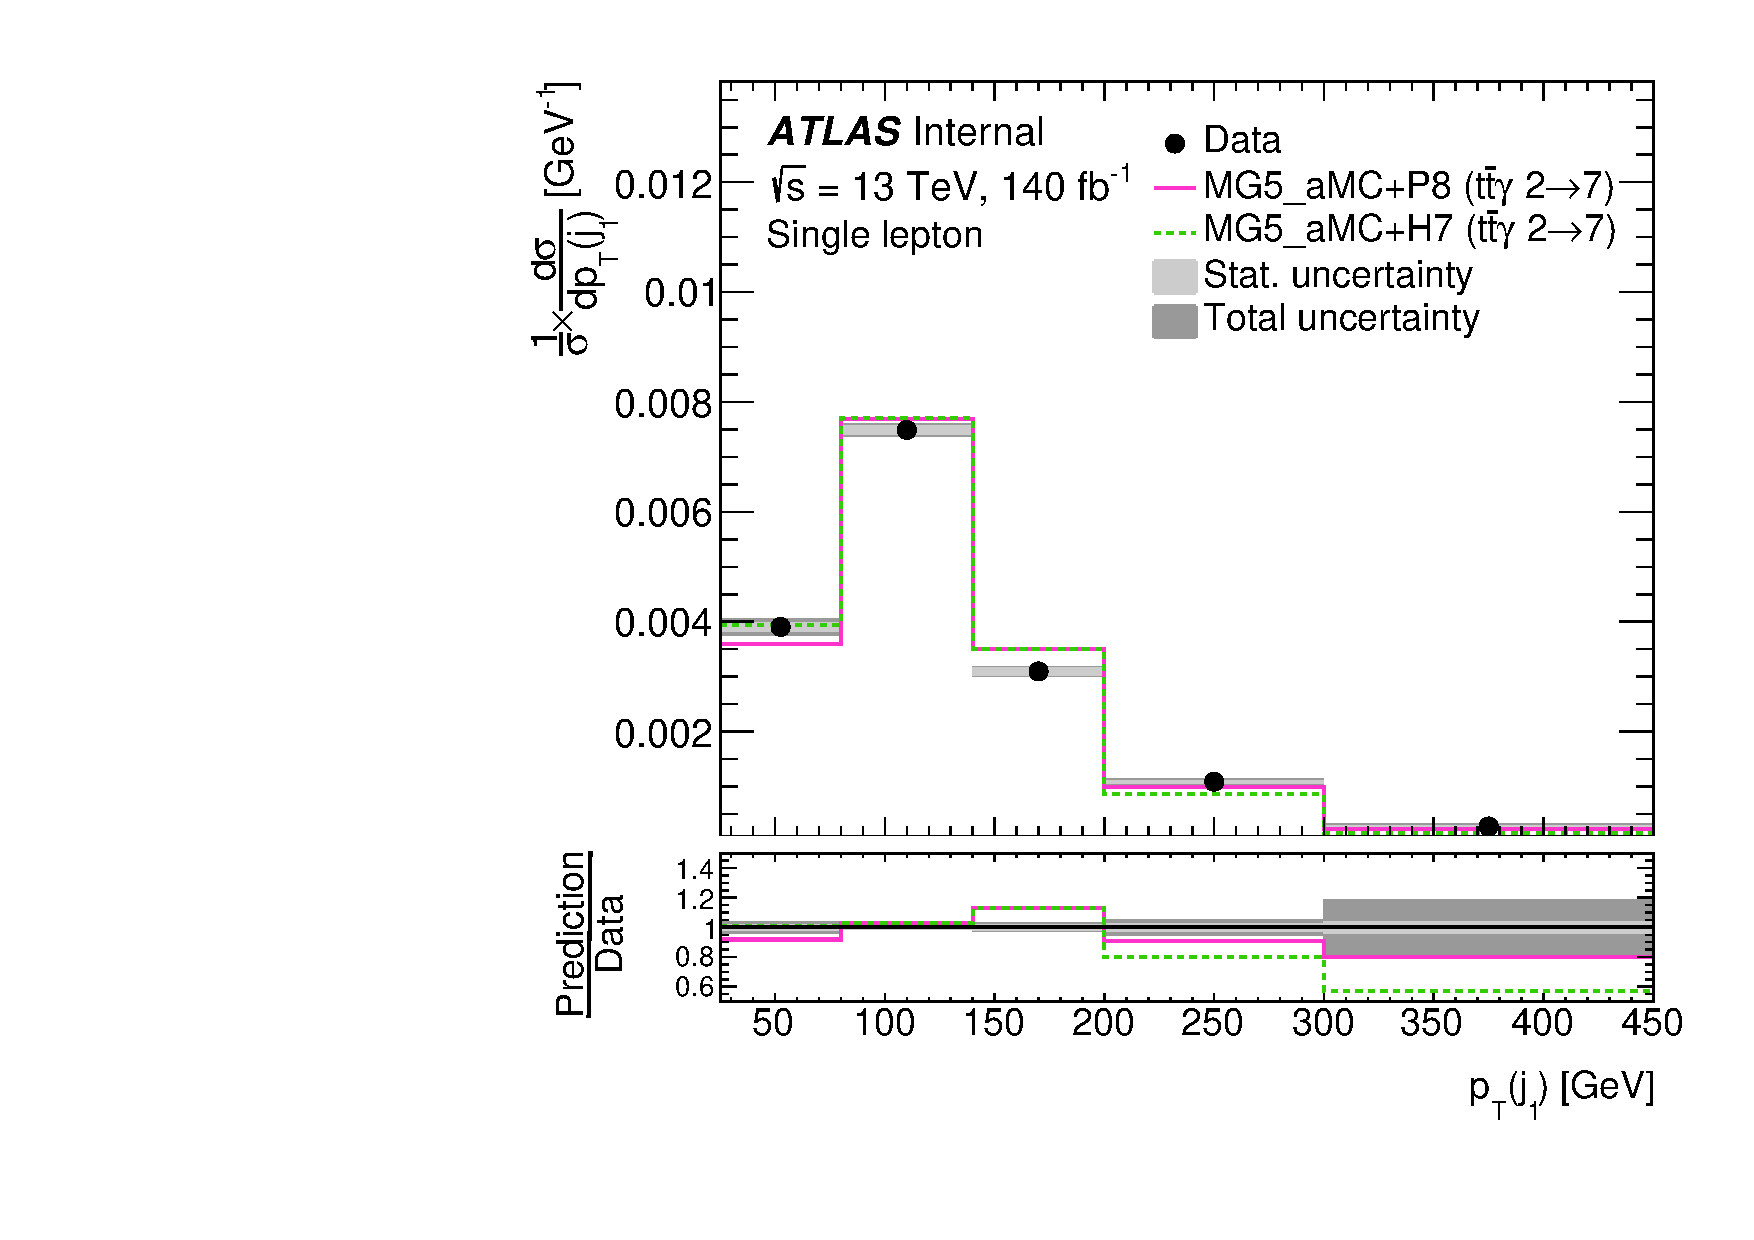
\includegraphics[width=0.33\textwidth]{figures/diff_xsec/normalized-unfolded-distributions/tty_total_ljet/SL_tty_total_ptj1_unfolded_normalized.pdf}%
  \caption{Normalised differential of the total \tty production and decay
  cross-section measured in the fiducial phase space in the single-lepton
  channel as a function of the photon \pt, photon $|\eta|$, $\Delta R_{min}
  (\gamma, b)$, $\Delta R (\gamma, \ell)$ and $\Delta_{min} R (j, \ell)$ (from
  left to right and top to bottom). Data are compared with MadGraph5\_aMC@NLO
  simulation interfaced with \PYTHIA[8] and \HERWIG[7]. The lower parts of each
  plot show the ratio of the prediction to the data. }
  \label{fig:tty_total_diff_Ljets_norm}
\end{figure}
\FloatBarrier

\begin{figure}[ht]
  \centering
  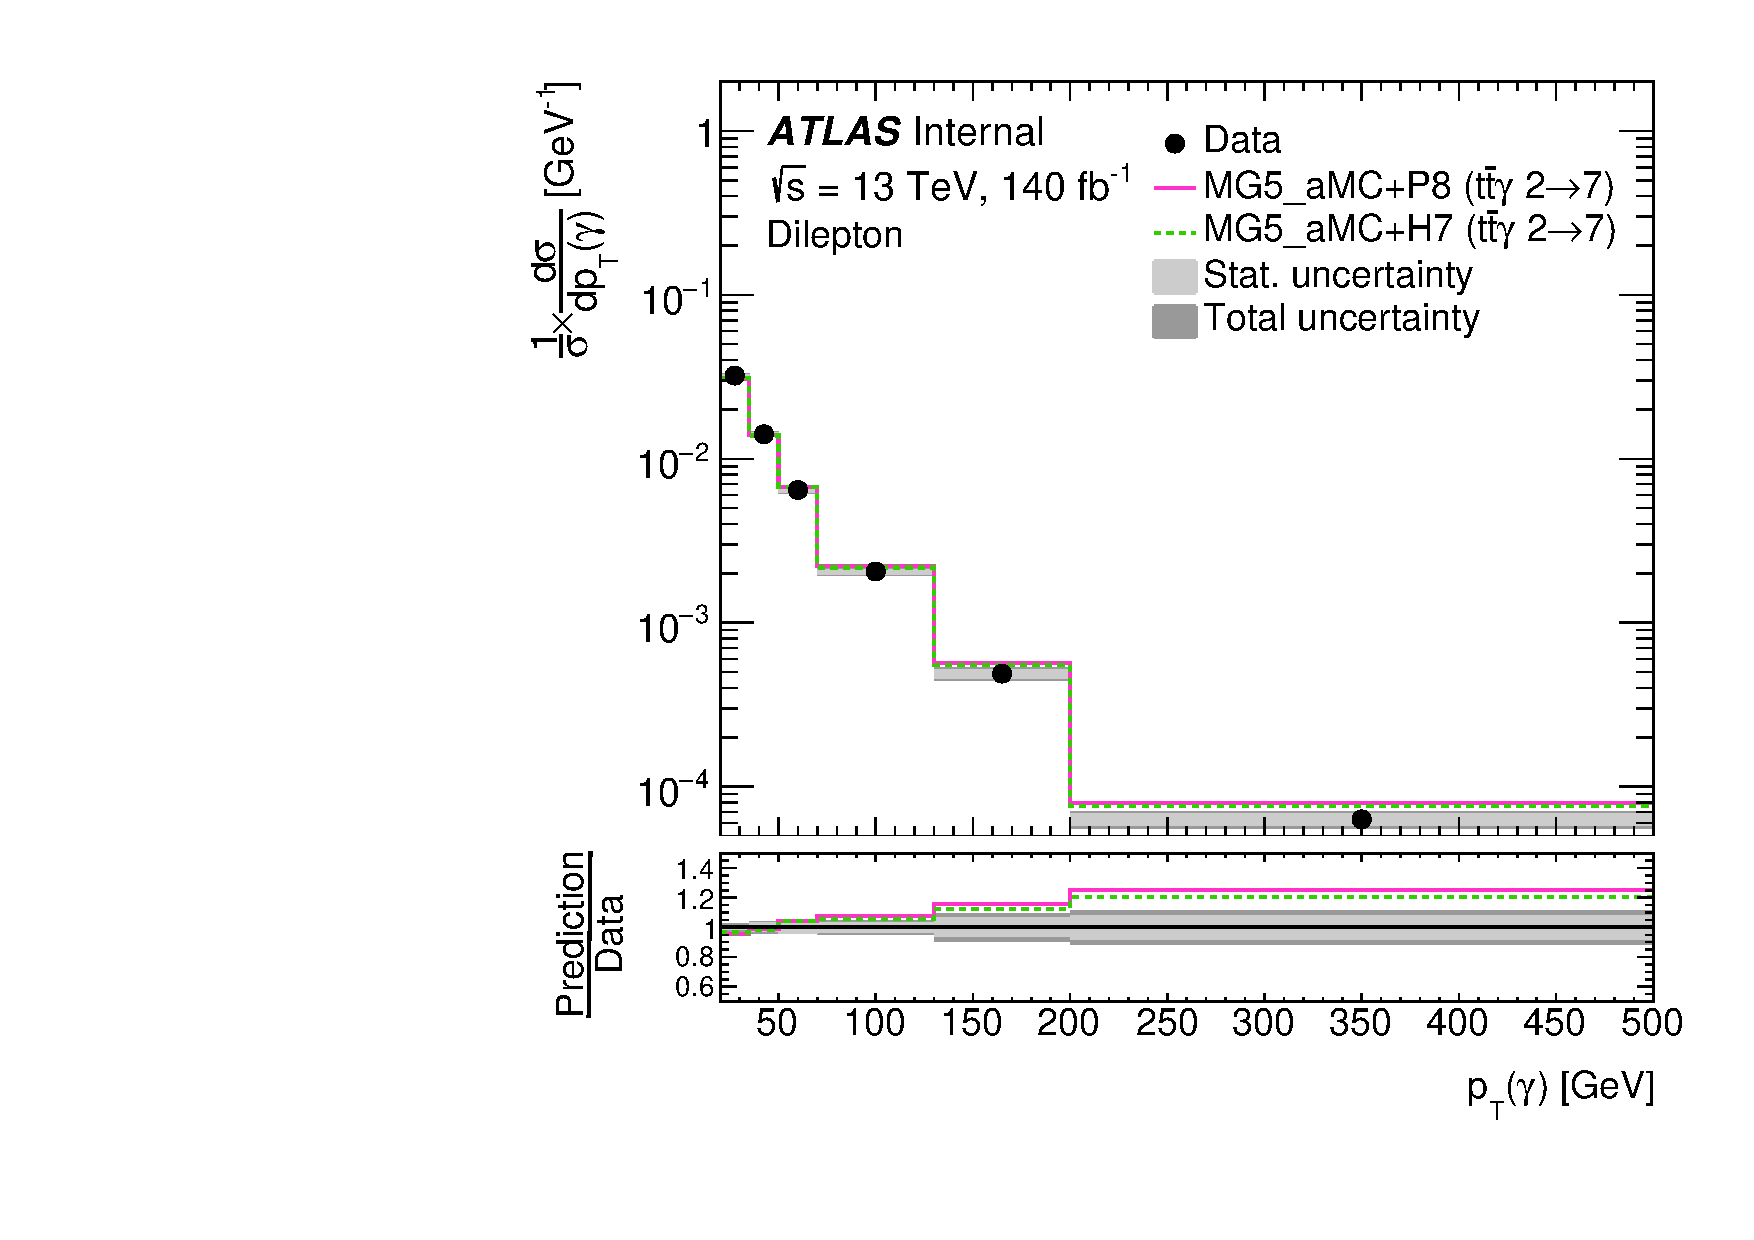
\includegraphics[width=0.33\textwidth]{figures/diff_xsec/normalized-unfolded-distributions/tty_total_dilep/DL_tty_total_pt_unfolded_normalized.pdf}%
  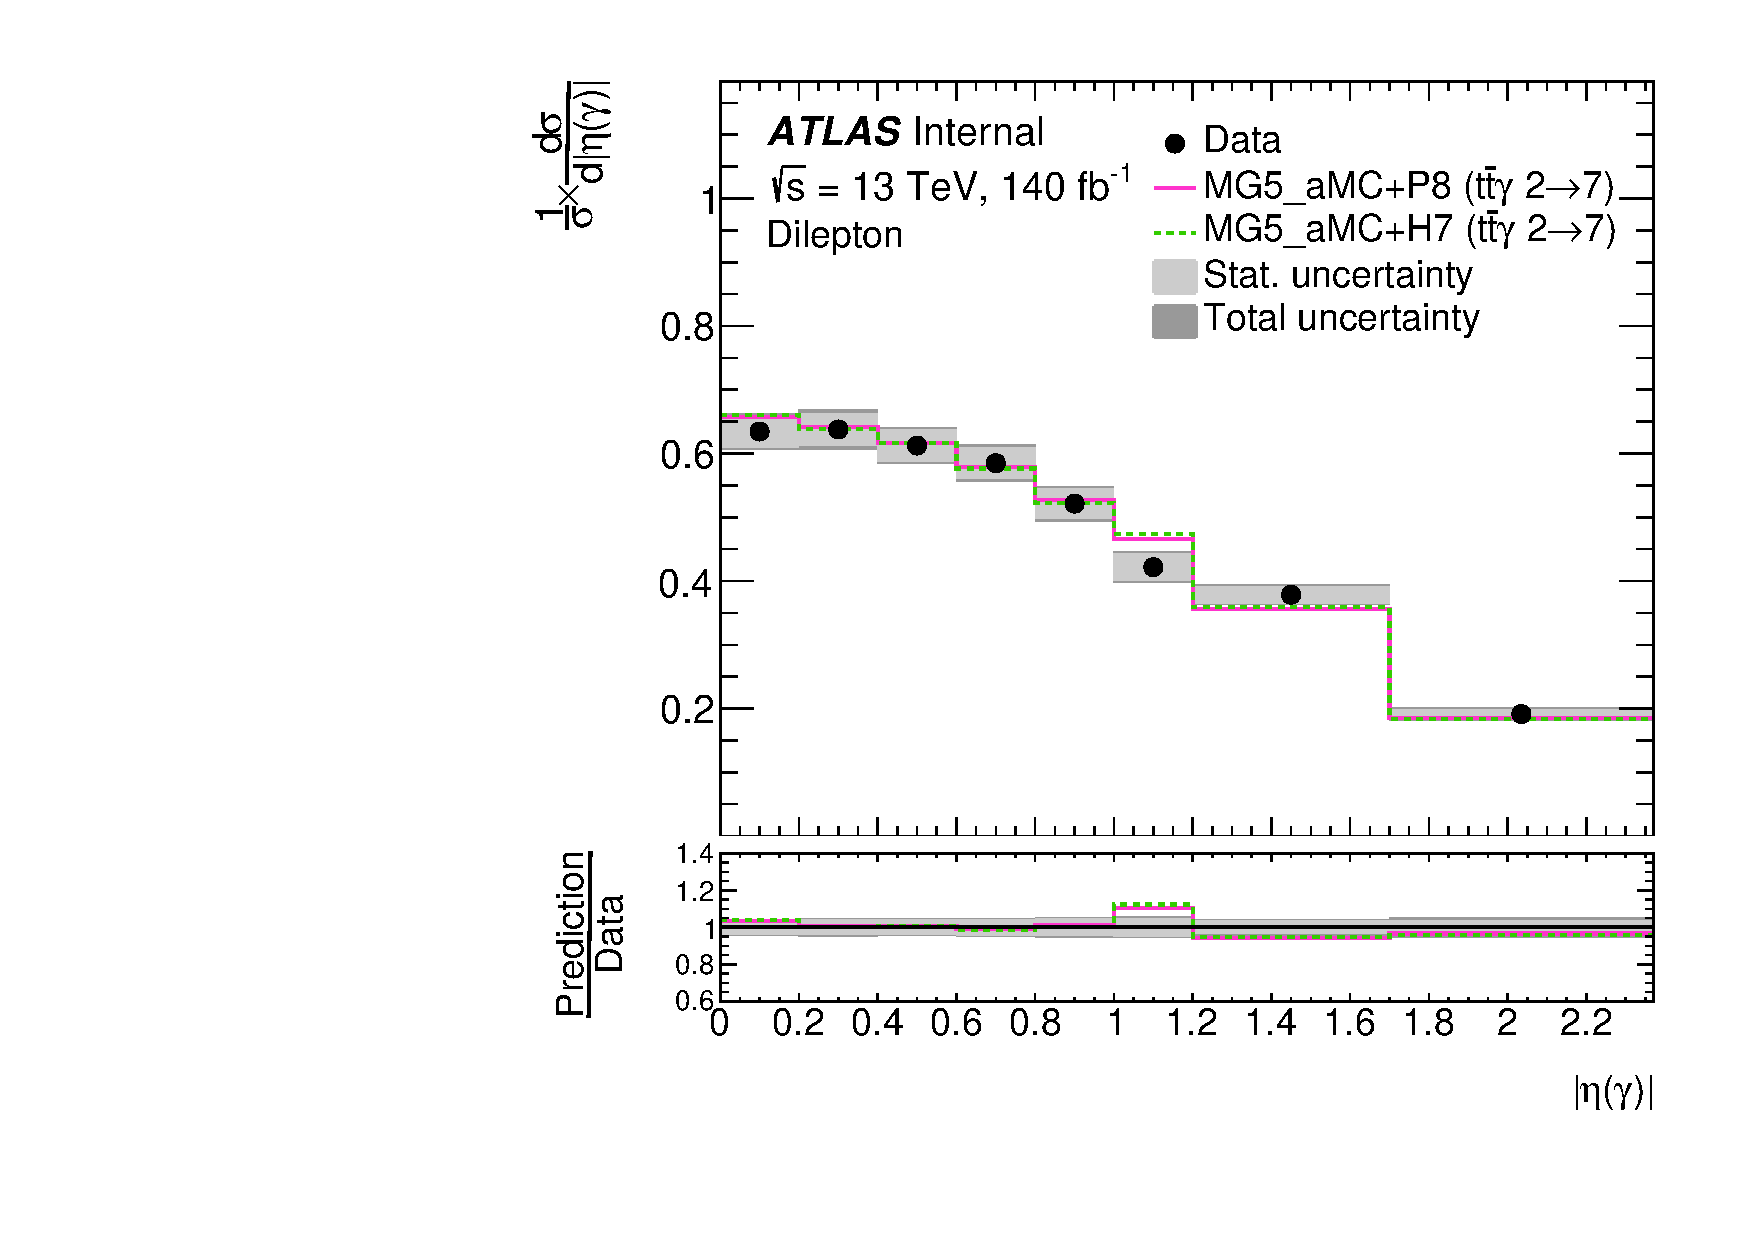
\includegraphics[width=0.33\textwidth]{figures/diff_xsec/normalized-unfolded-distributions/tty_total_dilep/DL_tty_total_eta_unfolded_normalized.pdf}%
  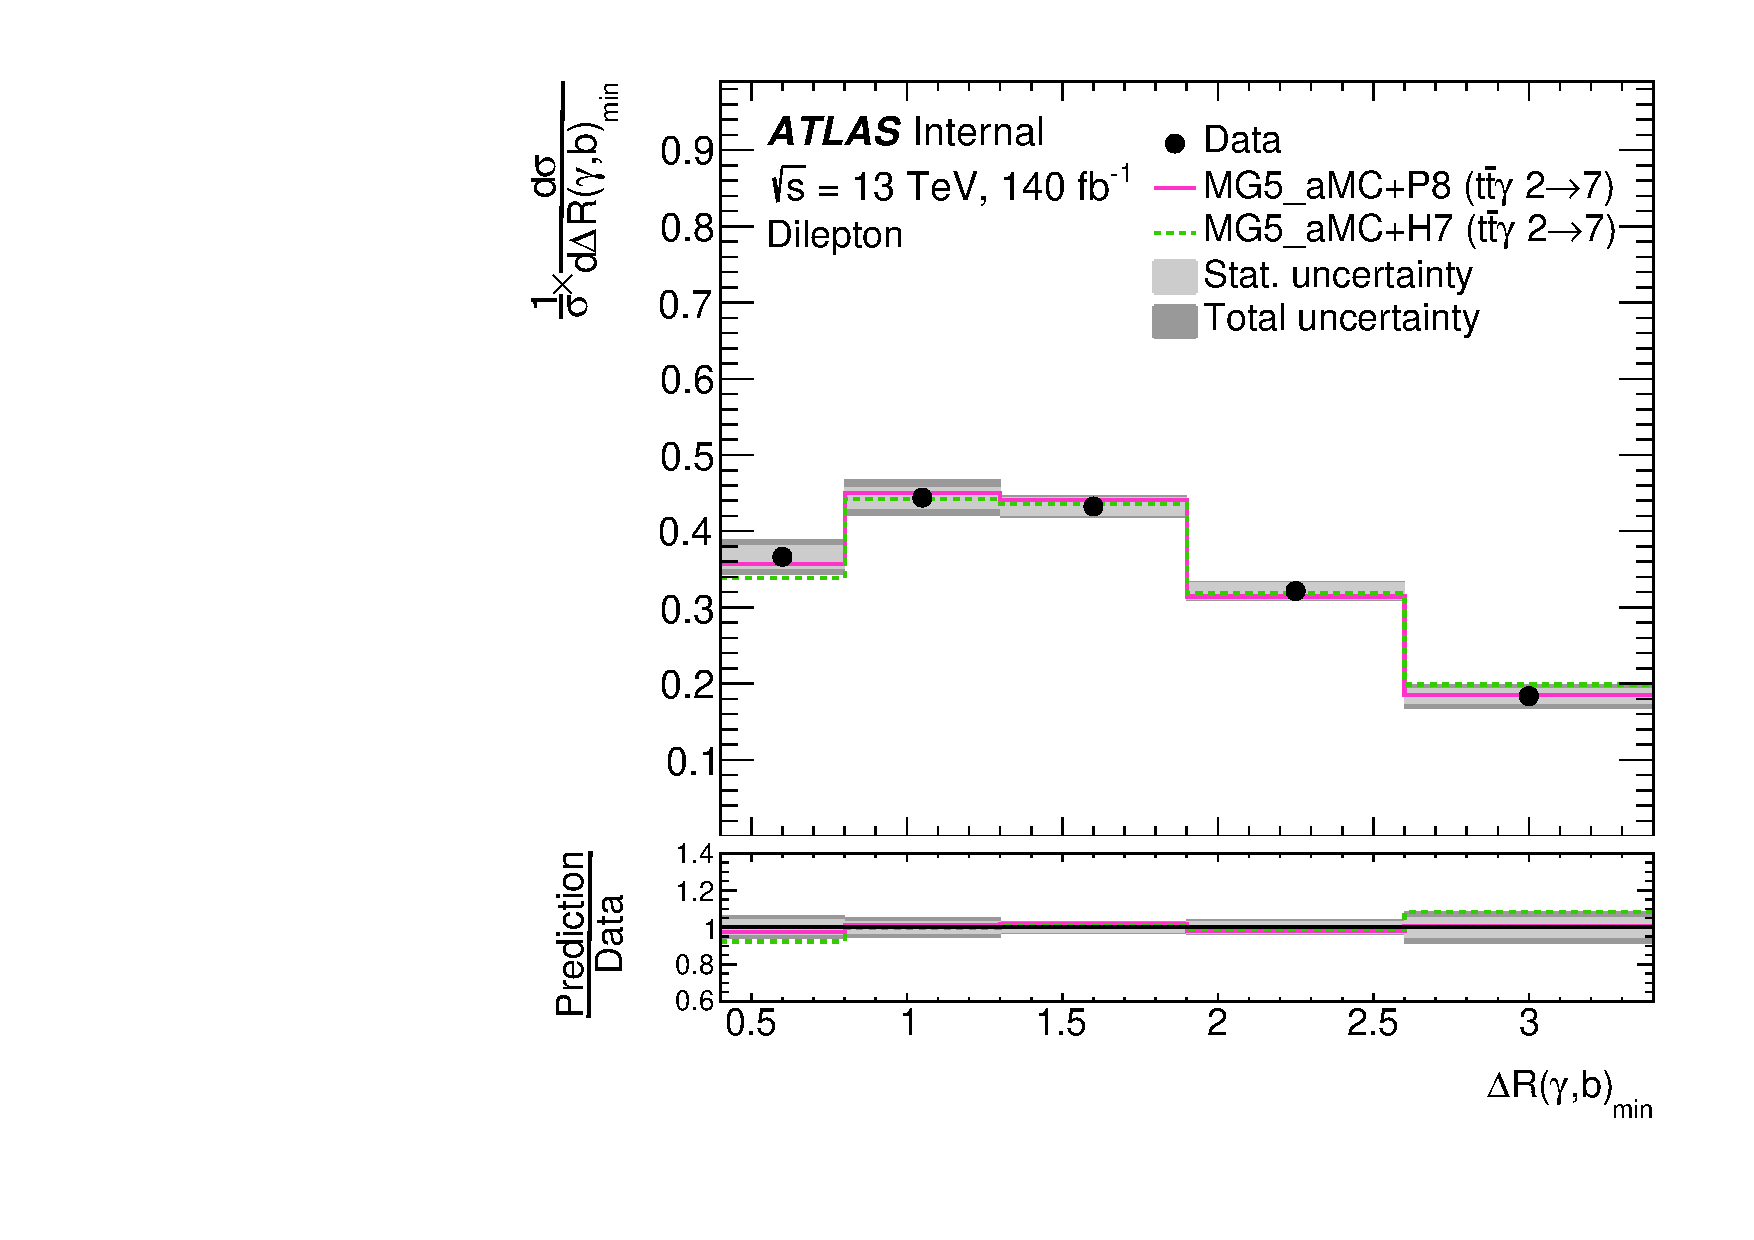
\includegraphics[width=0.33\textwidth]{figures/diff_xsec/normalized-unfolded-distributions/tty_total_dilep/DL_tty_total_drphb_unfolded_normalized.pdf}\\
  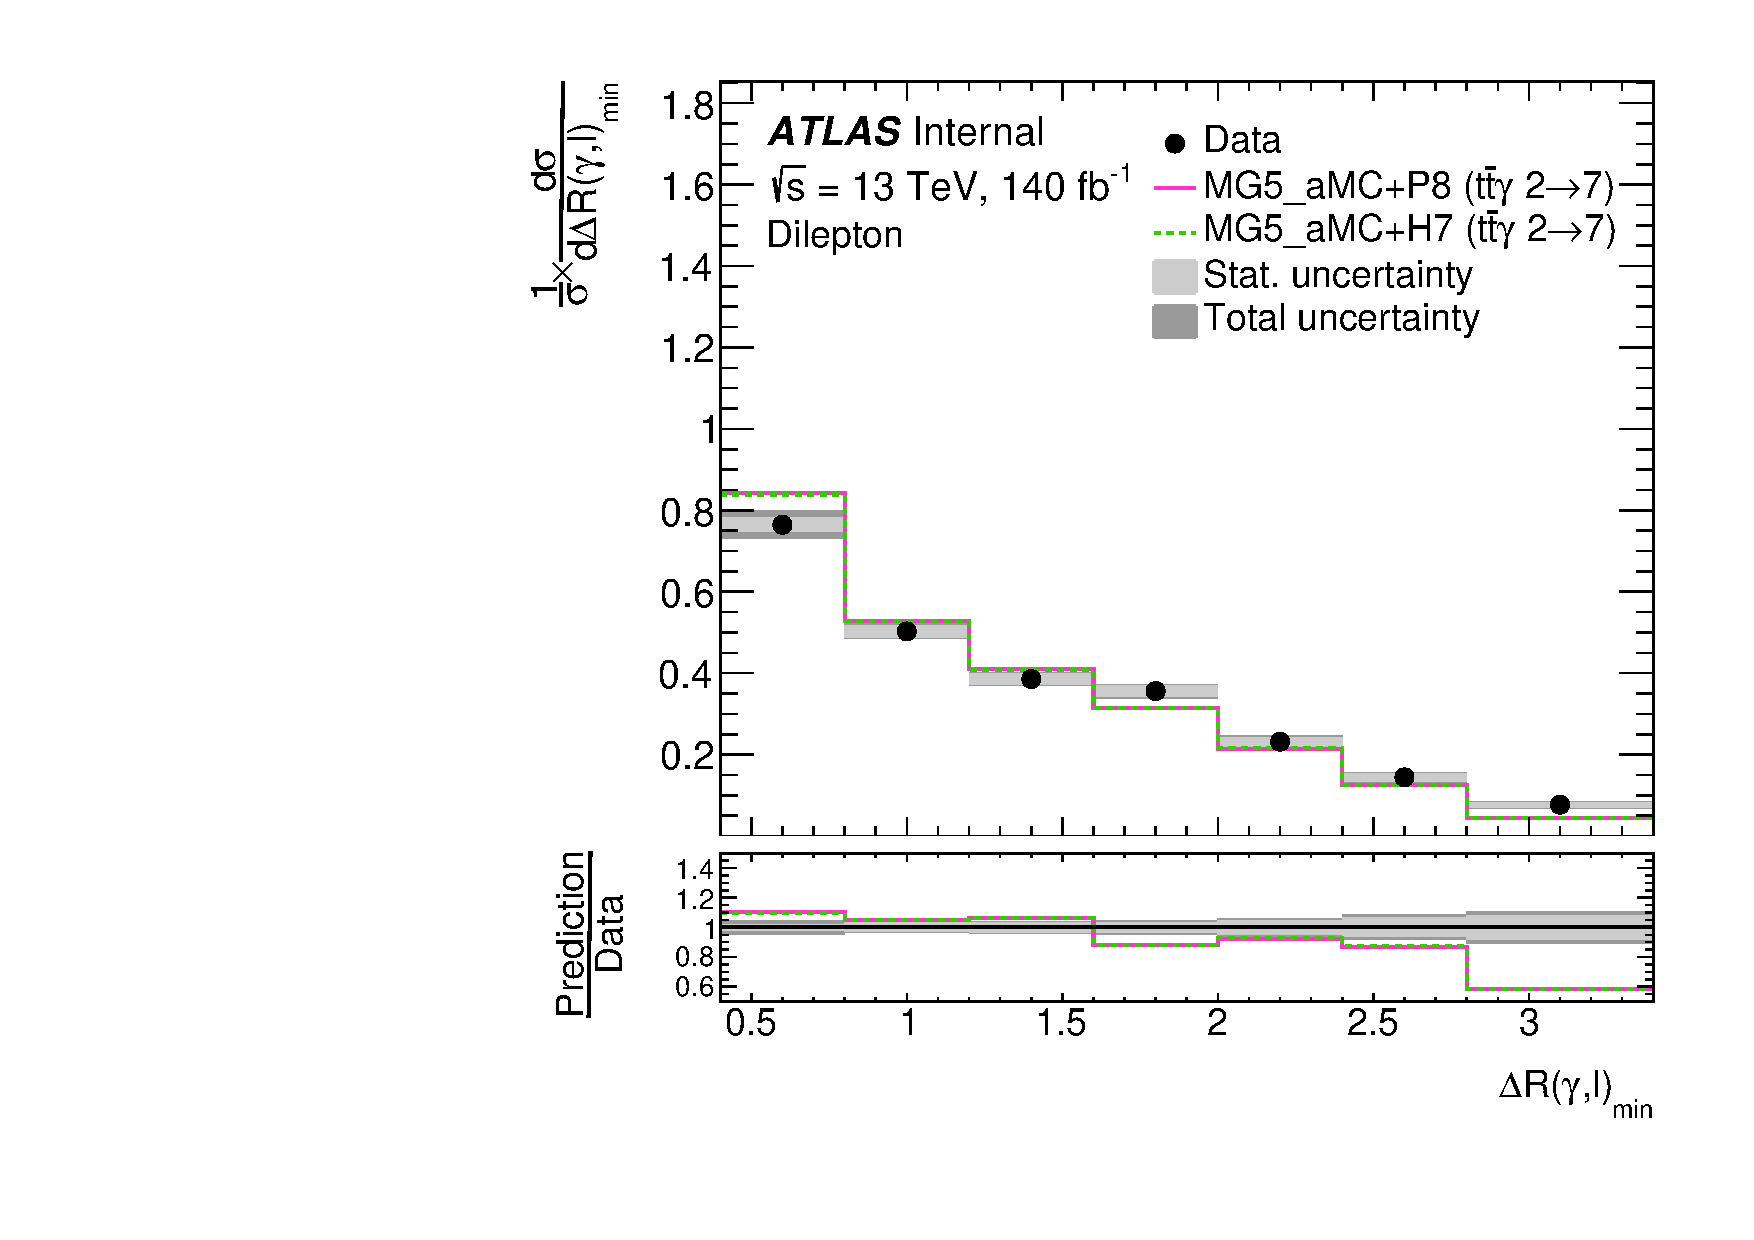
\includegraphics[width=0.33\textwidth]{figures/diff_xsec/normalized-unfolded-distributions/tty_total_dilep/DL_tty_total_drphl_unfolded_normalized.pdf}%
  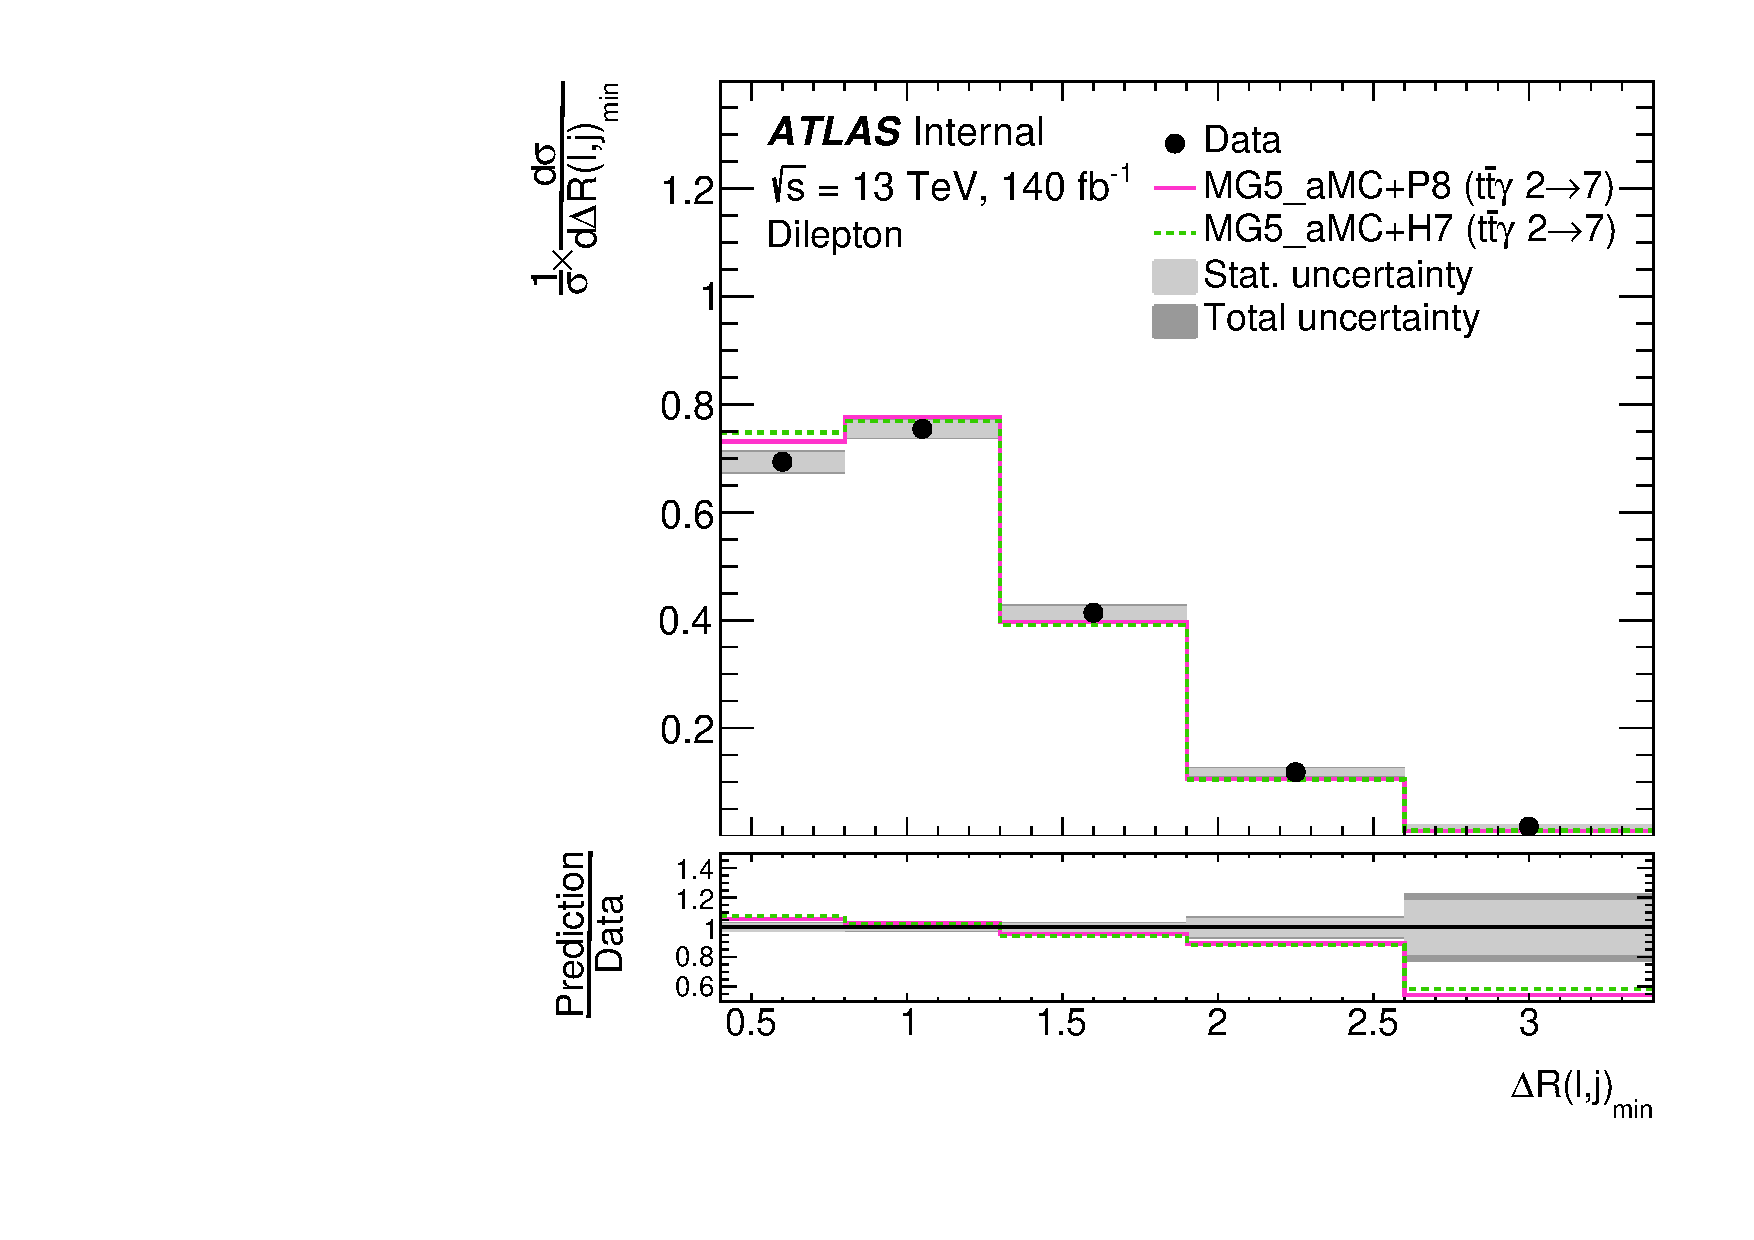
\includegraphics[width=0.33\textwidth]{figures/diff_xsec/normalized-unfolded-distributions/tty_total_dilep/DL_tty_total_drlj_unfolded_normalized.pdf}%
  \caption{Normalised differential of the total \tty production and decay
  cross-section measured in the fiducial phase space in the dilepton channel as
  a function of the photon \pt, photon $|\eta|$, $\Delta R_{min} (\gamma, b)$,
  $\Delta R (\gamma, \ell)$ and $\Delta_{min} R (j, \ell)$ (from left to right
  and top to bottom). Data are compared with MadGraph5\_aMC@NLO simulation
  interfaced with \PYTHIA[8] and \HERWIG[7]. The lower parts of each plot show
  the ratio of the prediction to the data.}
  \label{fig:tty_total_diff_DL1_norm}
\end{figure}
\FloatBarrier

\begin{figure}[ht]
  \centering
  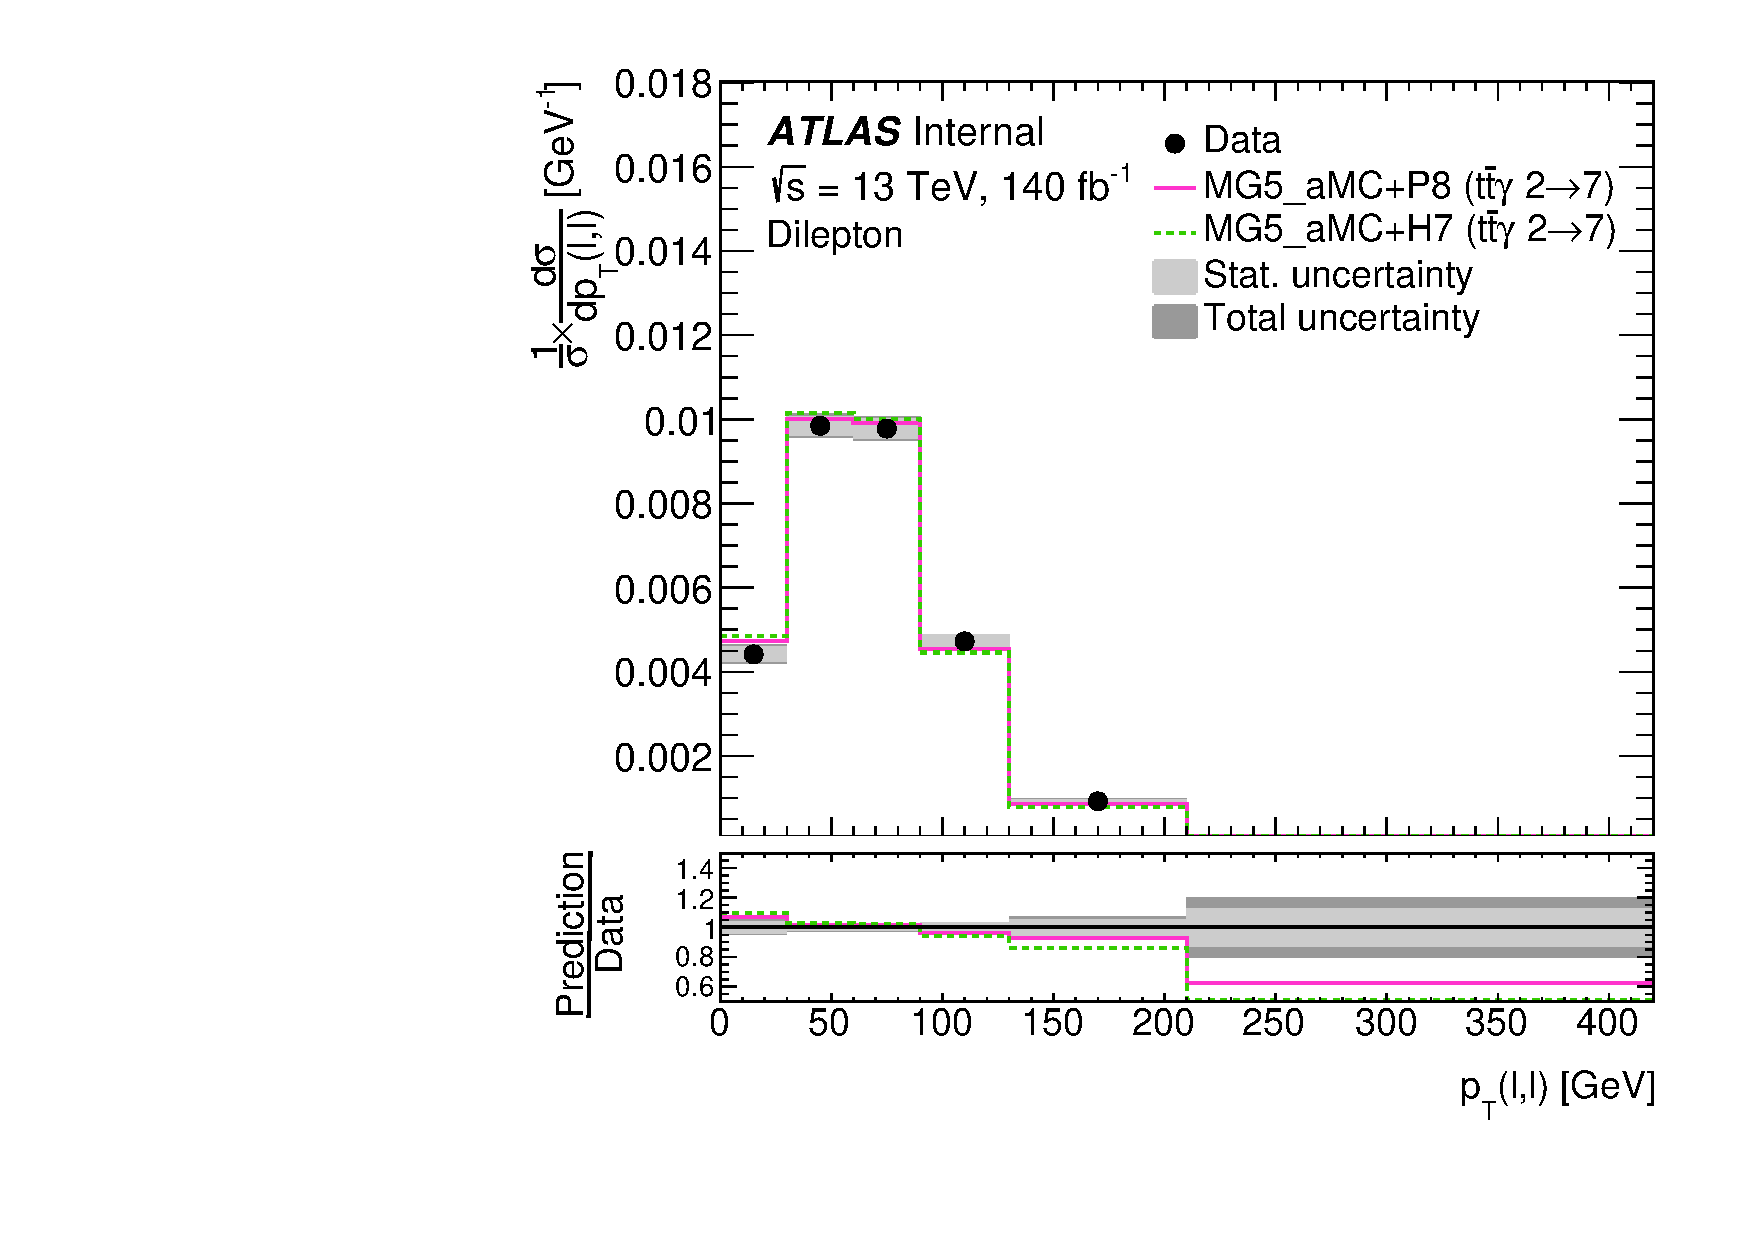
\includegraphics[width=0.33\textwidth]{figures/diff_xsec/normalized-unfolded-distributions/tty_total_dilep/DL_tty_total_ptll_unfolded_normalized.pdf}%
  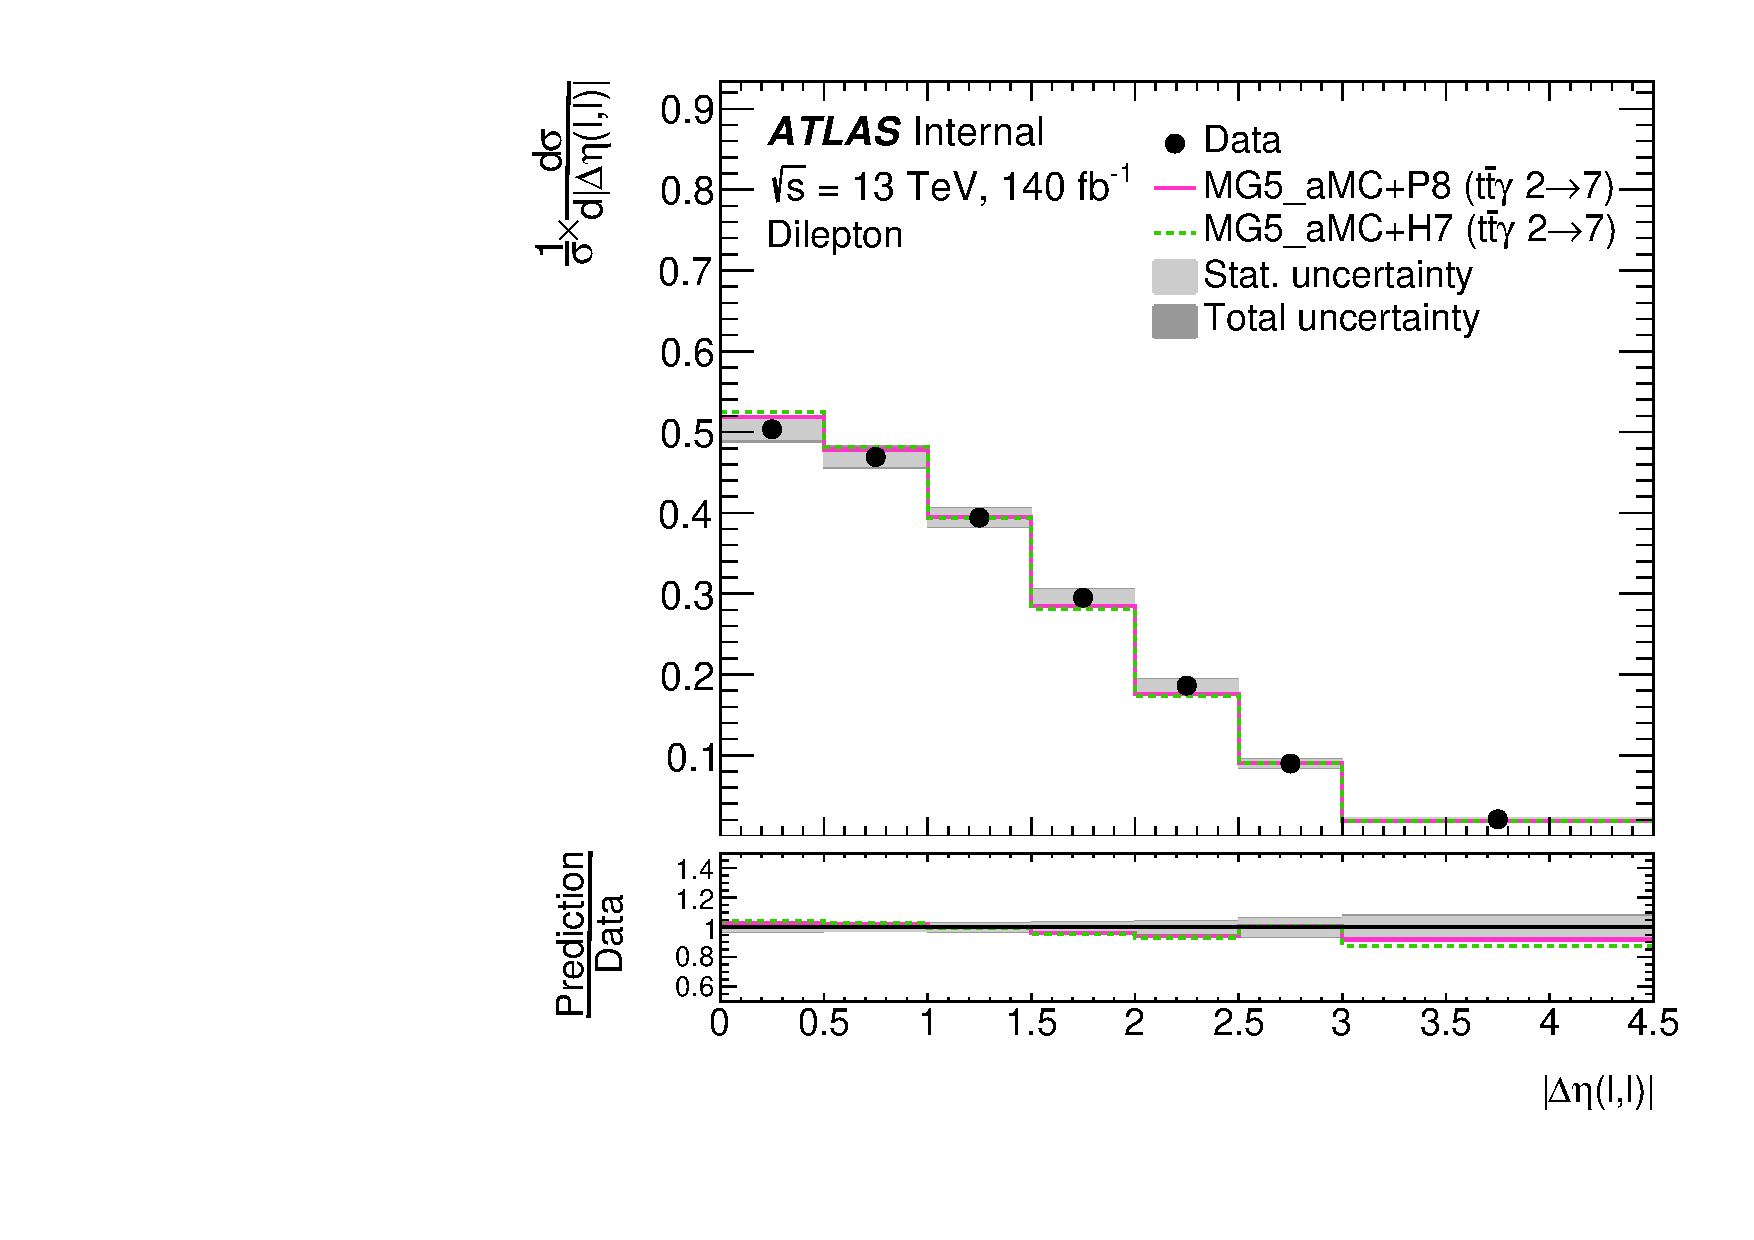
\includegraphics[width=0.33\textwidth]{figures/diff_xsec/normalized-unfolded-distributions/tty_total_dilep/DL_tty_total_dEtall_unfolded_normalized.pdf}%
  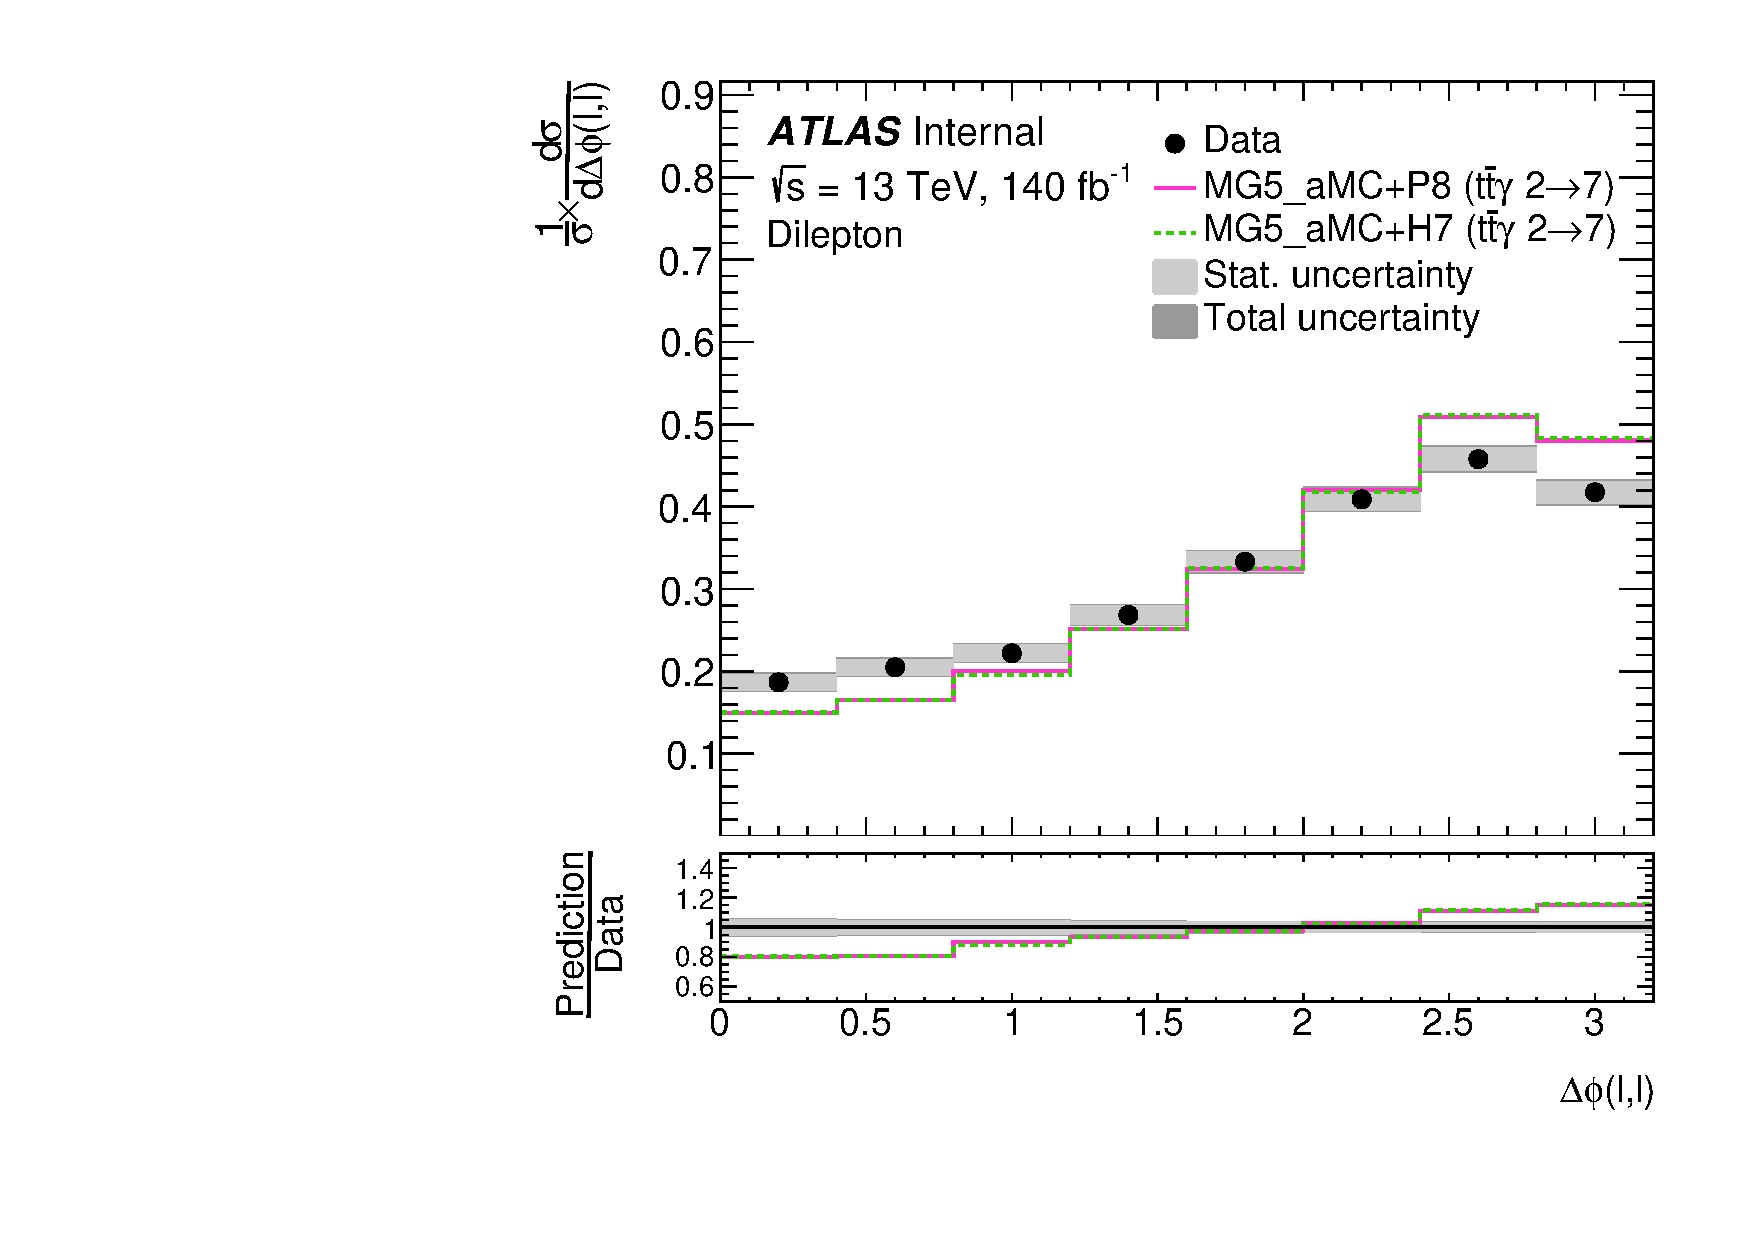
\includegraphics[width=0.33\textwidth]{figures/diff_xsec/normalized-unfolded-distributions/tty_total_dilep/DL_tty_total_dPhill_unfolded_normalized.pdf}\\
  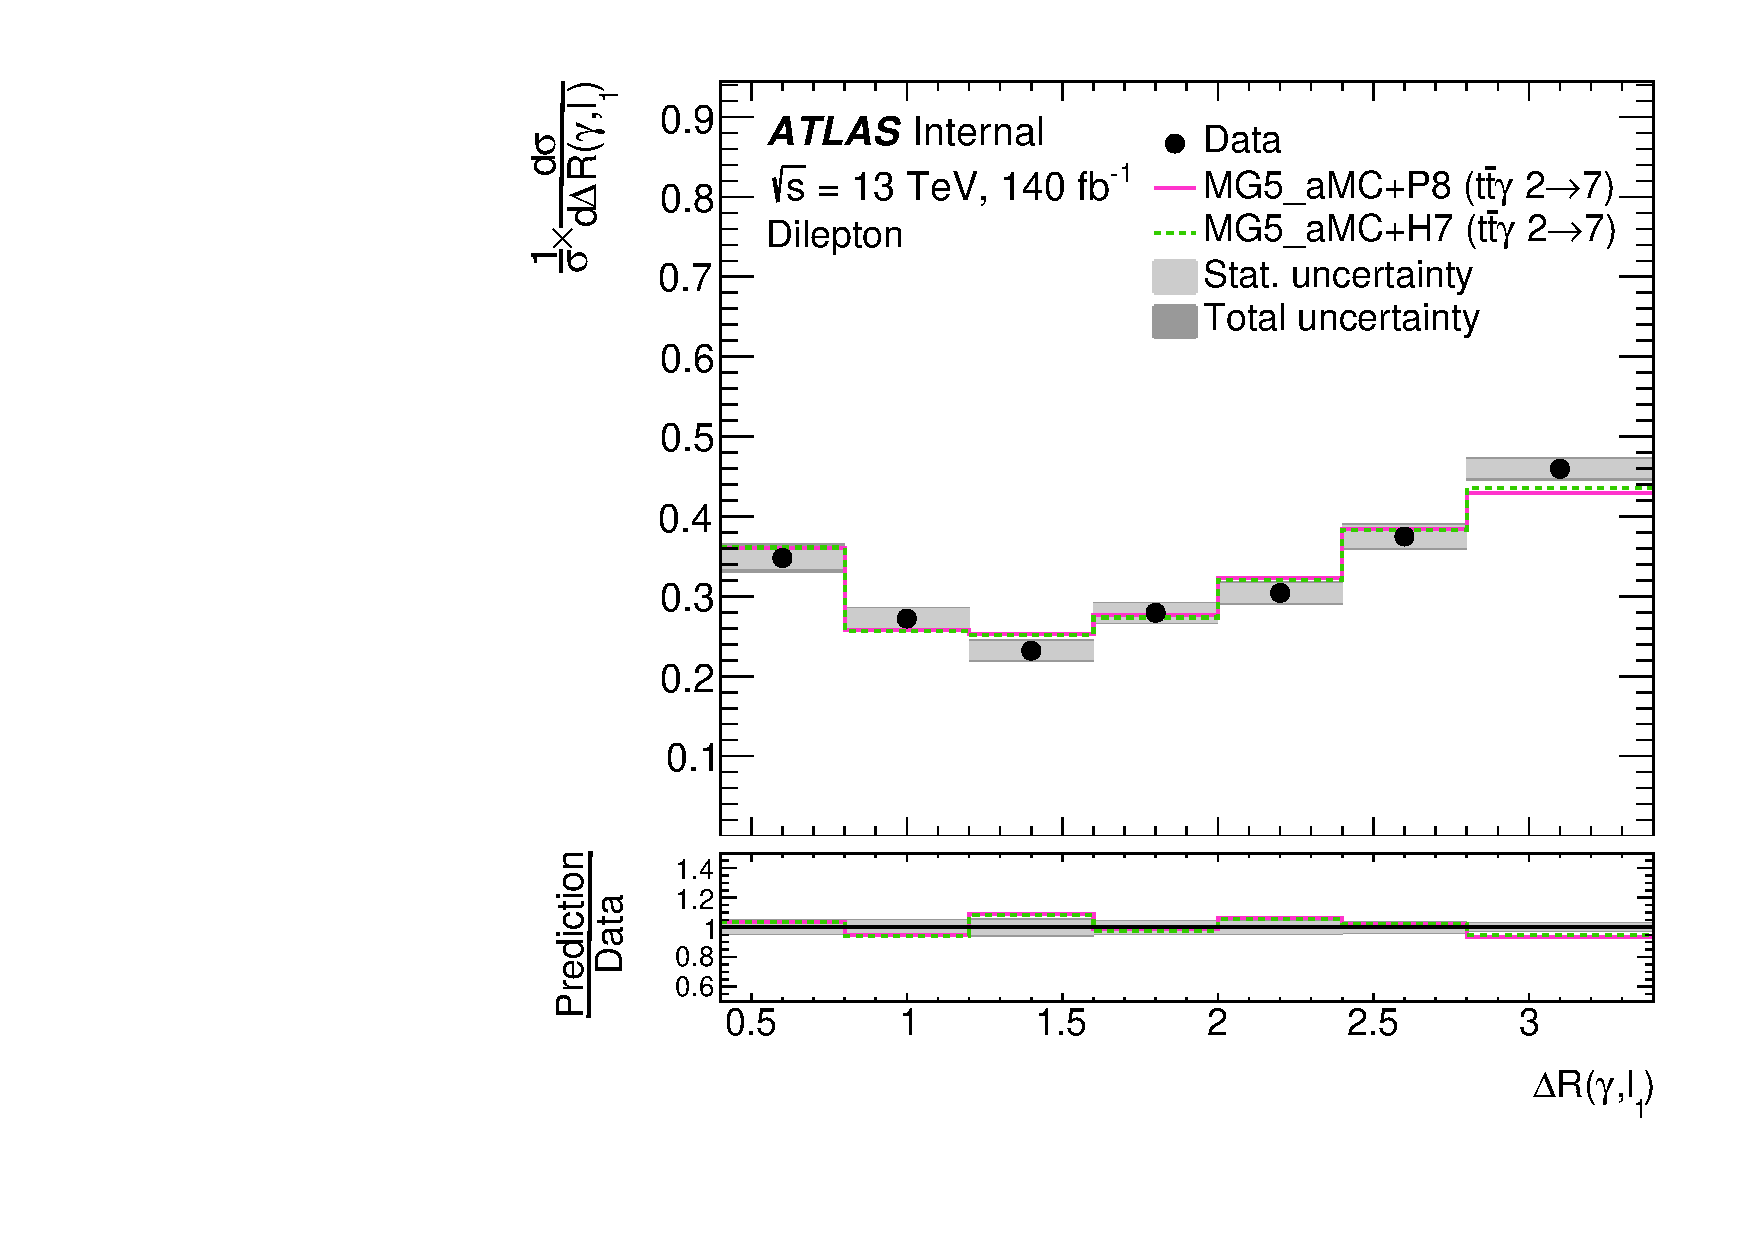
\includegraphics[width=0.33\textwidth]{figures/diff_xsec/normalized-unfolded-distributions/tty_total_dilep/DL_tty_total_drphl1_unfolded_normalized.pdf}%
  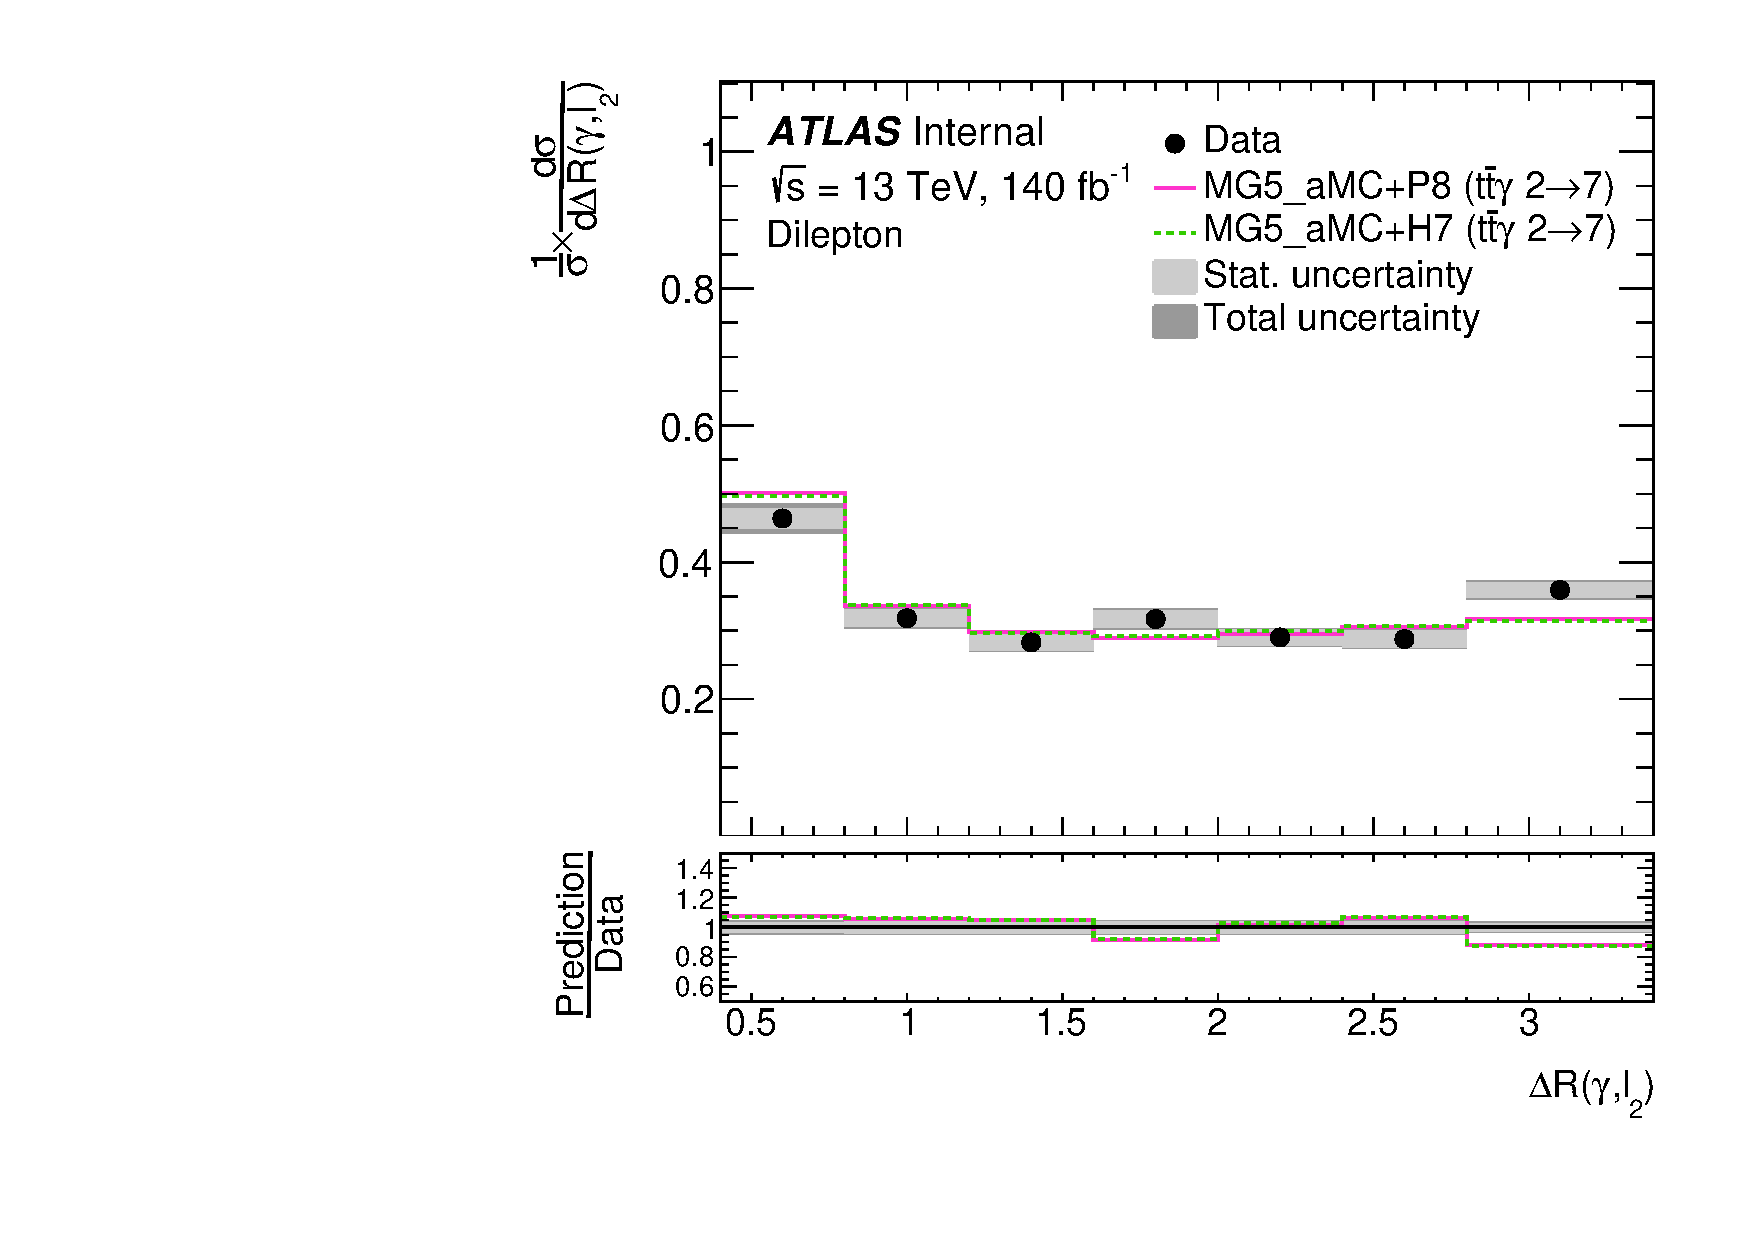
\includegraphics[width=0.33\textwidth]{figures/diff_xsec/normalized-unfolded-distributions/tty_total_dilep/DL_tty_total_drphl2_unfolded_normalized.pdf}%
  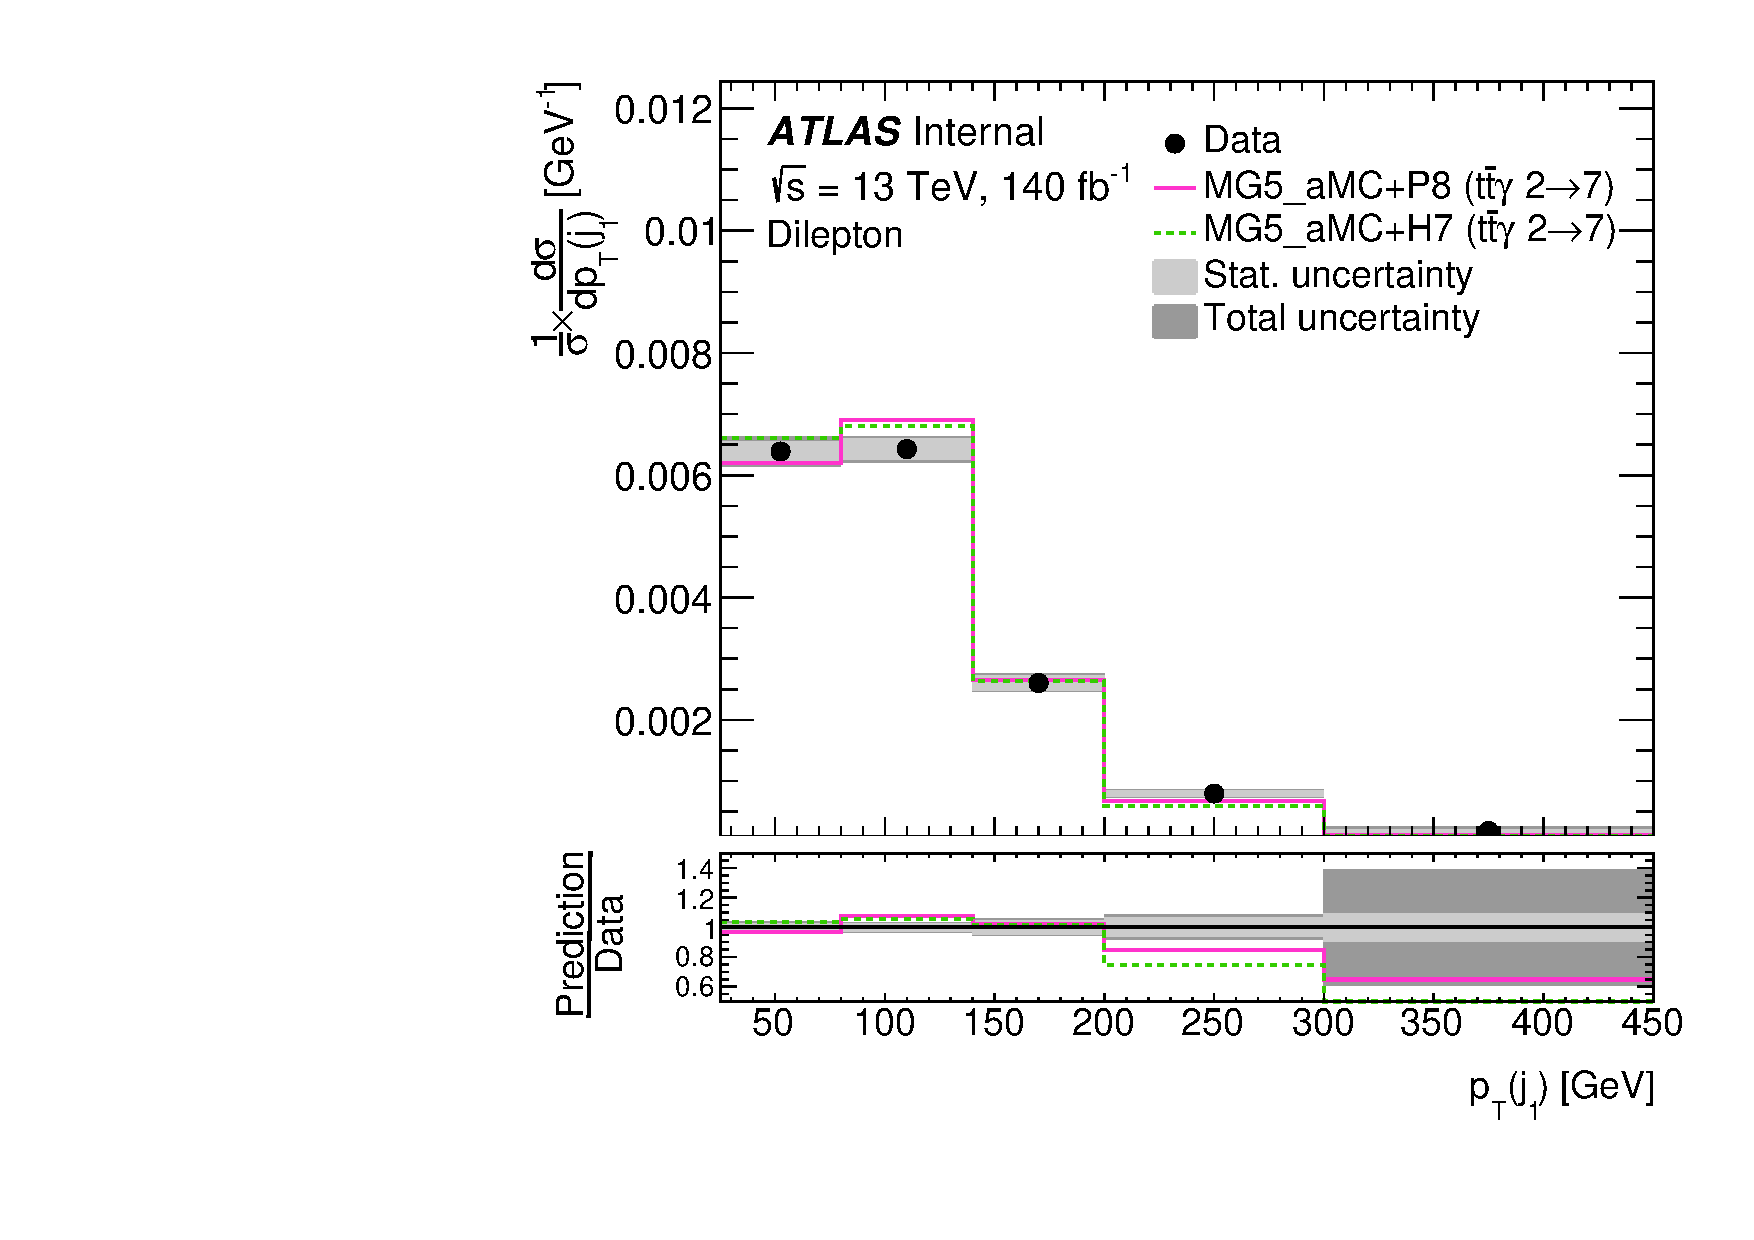
\includegraphics[width=0.33\textwidth]{figures/diff_xsec/normalized-unfolded-distributions/tty_total_dilep/DL_tty_total_ptj1_unfolded_normalized.pdf}%
    \caption{Normalised differential cross-section of the \tty total measured in the fiducial phase space in the dilepton channel as a function of the scalar sum of the \pt of the leptons, $|\Delta \eta(\ell\ell)|$, $\Delta \phi (\ell\ell)$, $\Delta R (\gamma, \ell_1)$, $\Delta R (\gamma, \ell_2)$ and leading jet \pt (from left to right and top to bottom). Data are compared with MadGraph5\_aMC@NLO simulation interfaced with \PYTHIA[8] and \HERWIG[7]. The lower parts of each plot show the ratio of the prediction to the data.}
  \label{fig:tty_total_diff_DL2_norm}
\end{figure}
\FloatBarrier

\begin{figure}[ht]
  \centering
  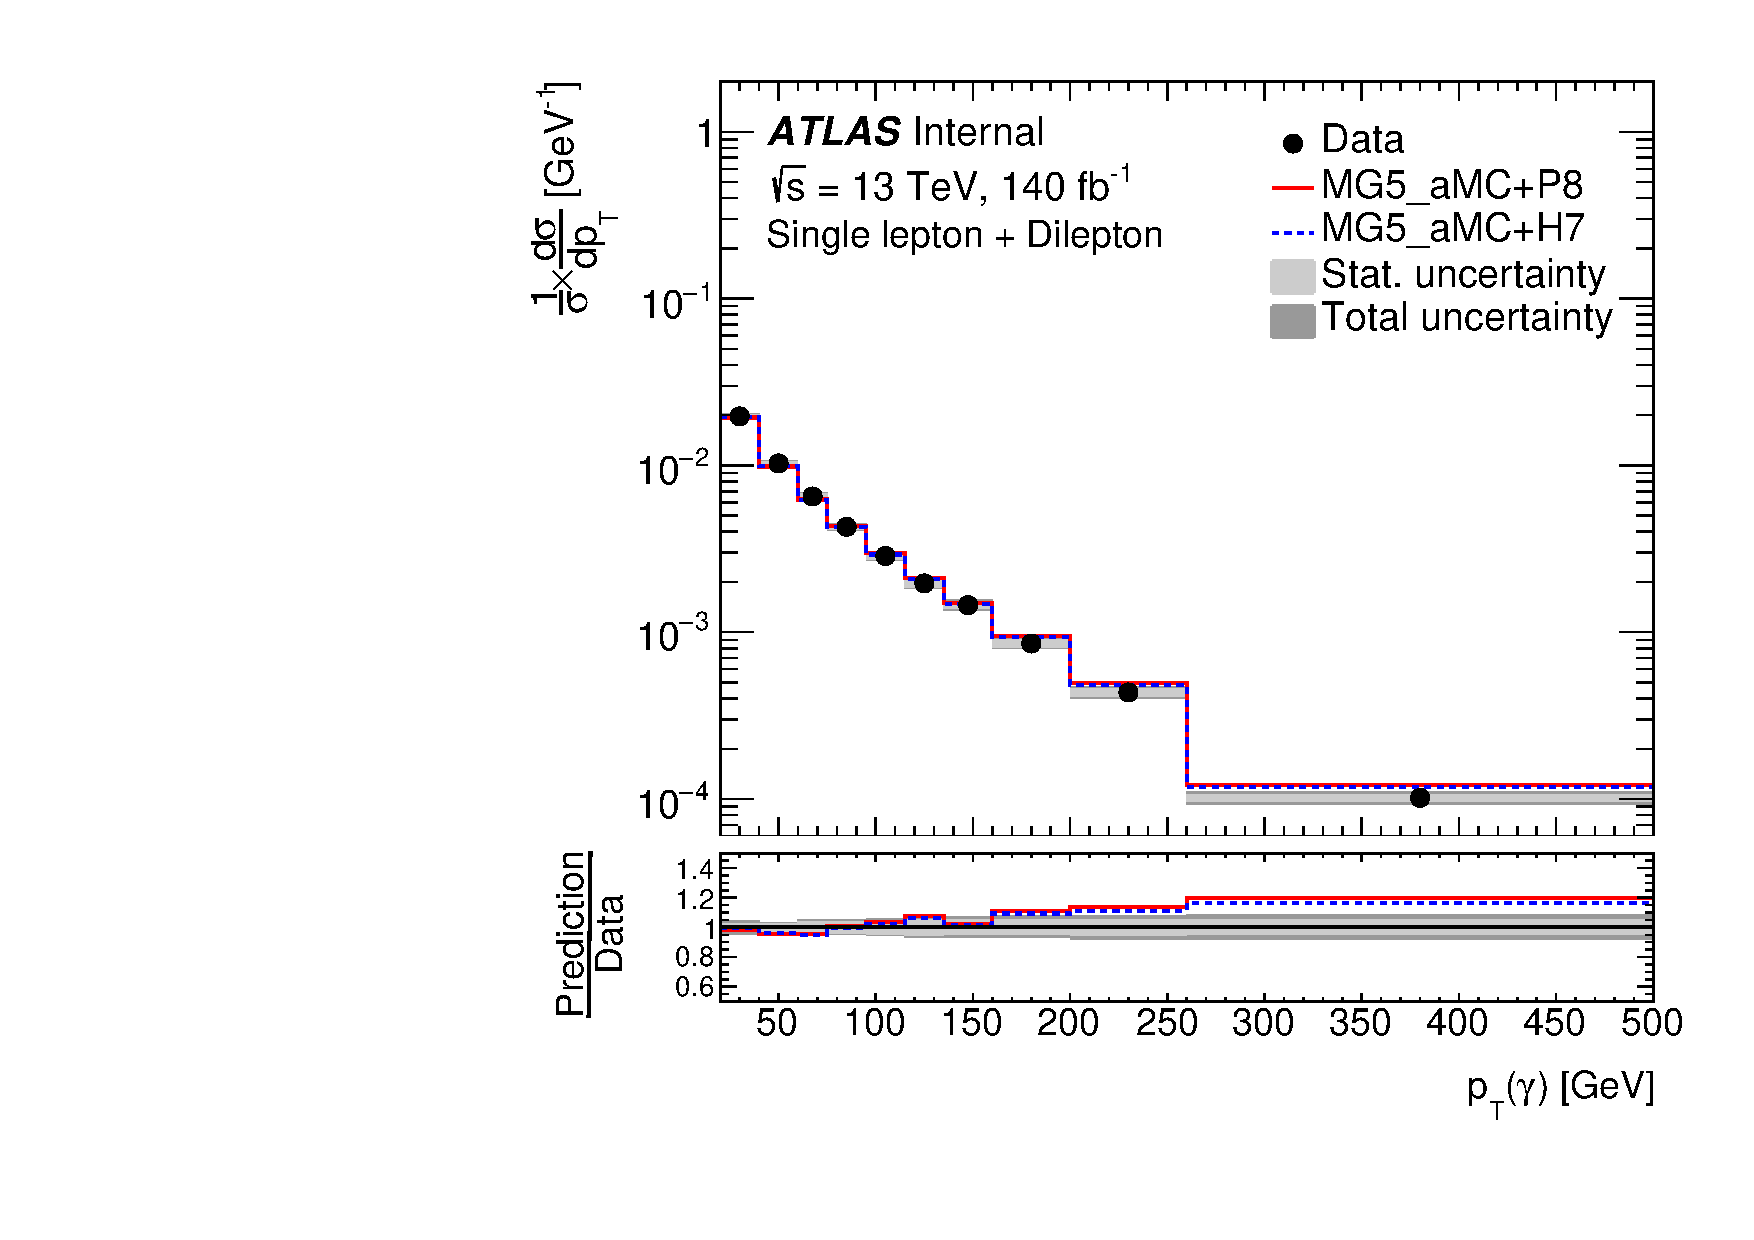
\includegraphics[width=0.33\textwidth]{figures/diff_xsec/normalized-unfolded-distributions/tty_prod_SLDL/tty_pt_UnfoldedData.pdf}%
  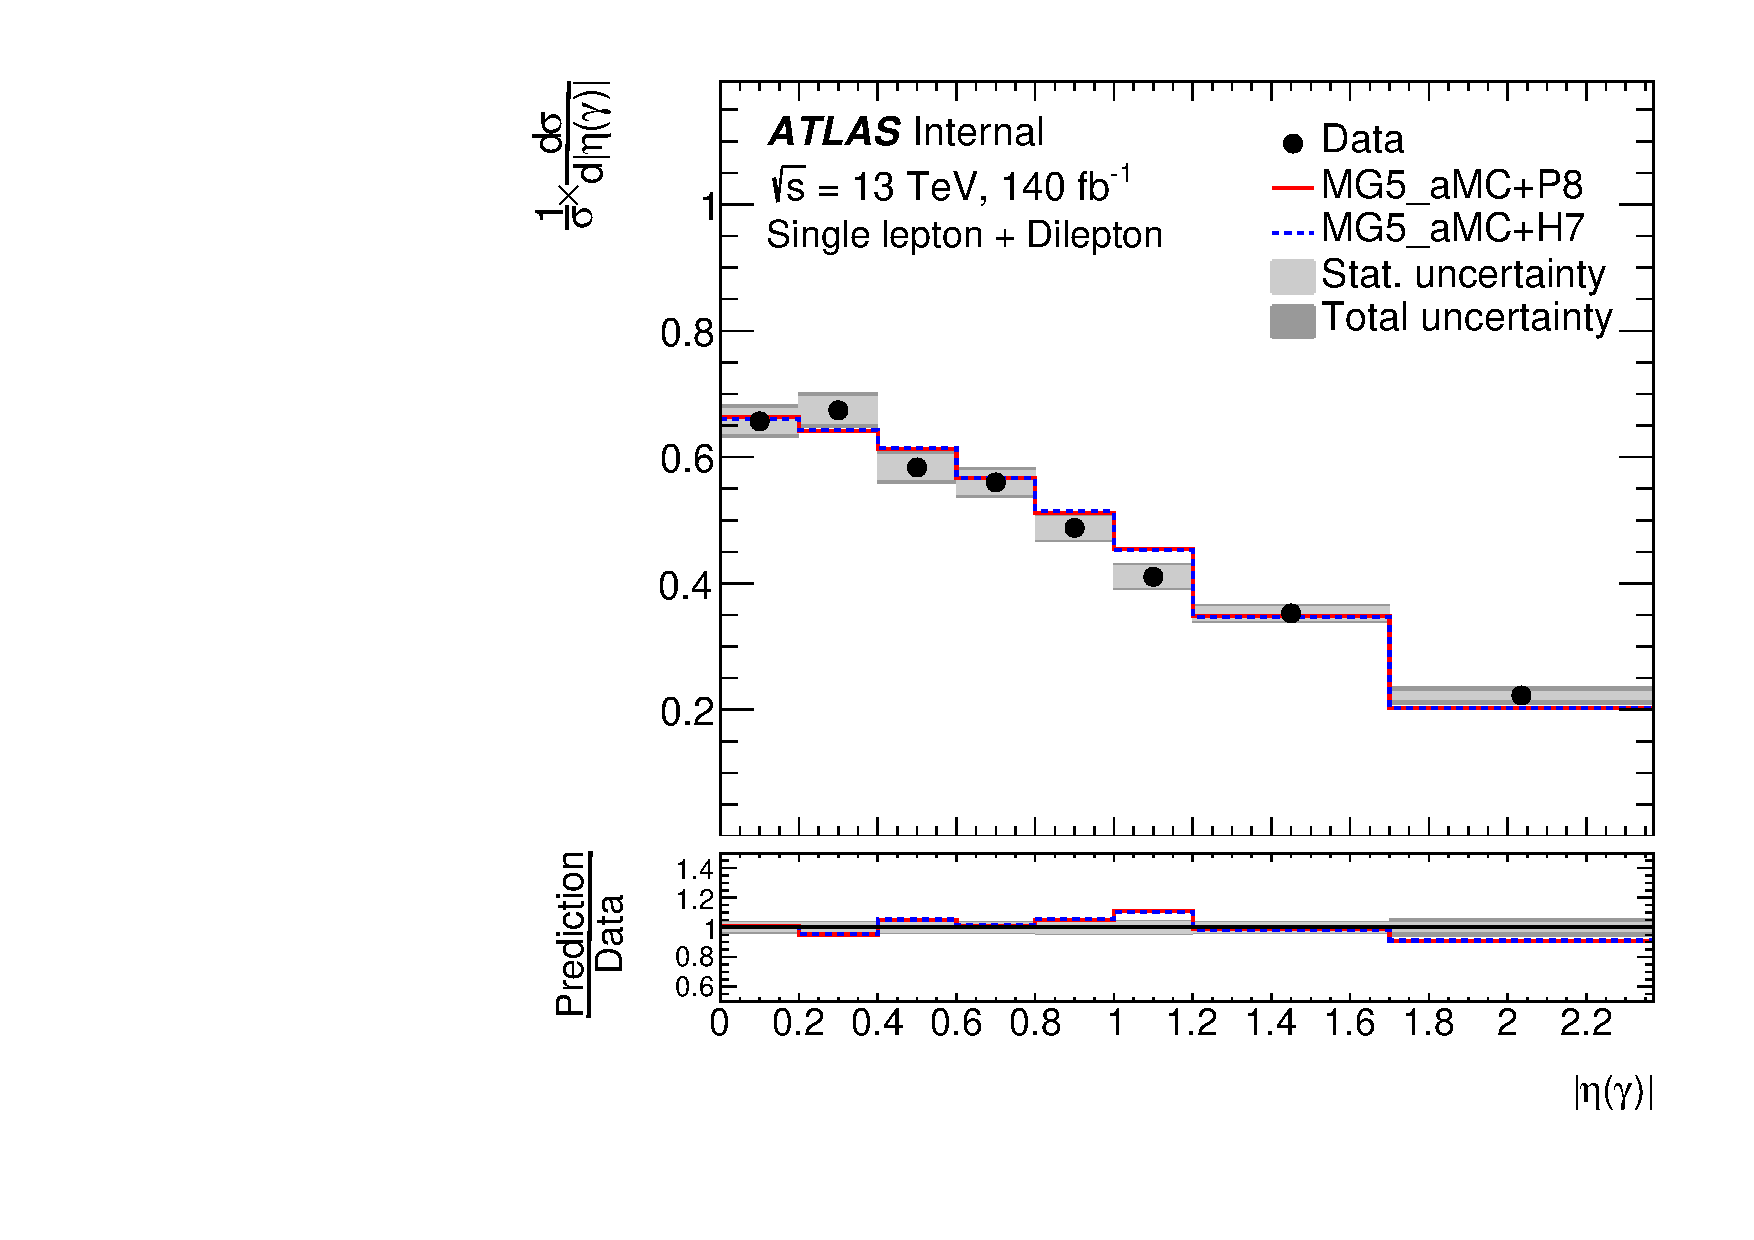
\includegraphics[width=0.33\textwidth]{figures/diff_xsec/normalized-unfolded-distributions/tty_prod_SLDL/tty_eta_UnfoldedData.pdf}%
  \caption{Normalised differential of the \tty production 
  cross-section measured in a combined single lepton and dilepton fiducial phase space as a function of the photon \pt, photon $|\eta|$.
  Data are compared with MadGraph5\_aMC@NLO
  simulation interfaced with \PYTHIA[8] and \HERWIG[7]. The lower parts of each
  plot show the ratio of the prediction to the data. }

  \label{fig:tty_prod_diff_SLDL_norm}
\end{figure}
\FloatBarrier


%%%%%%%%%%%%%%%%%%%%%%%%%%%%%%%%%%%%%%%%%%%%%%%%%%%%%%%%%%%%%%%%%%%%%%%%%%%%%%%%
%%%%%%%%% grouped impact %%%%%%%%%%%%%%%%%%%%%%%%%%%%%%%%%%%%%%%%%%%%%%%%%%%%%%%
%%%%%%%%%%%%%%%%%%%%%%%%%%%%%%%%%%%%%%%%%%%%%%%%%%%%%%%%%%%%%%%%%%%%%%%%%%%%%%%%

%%%%%%%%%%%%%%%%%%%%%%%%%%%%%%%%%% SLDL tty production %%%%%%%%%%%%%%%%%%%%%%%%%%%%%%%%%%%%%%%%%%%%%
\begin{figure}[ht]
  \centering
  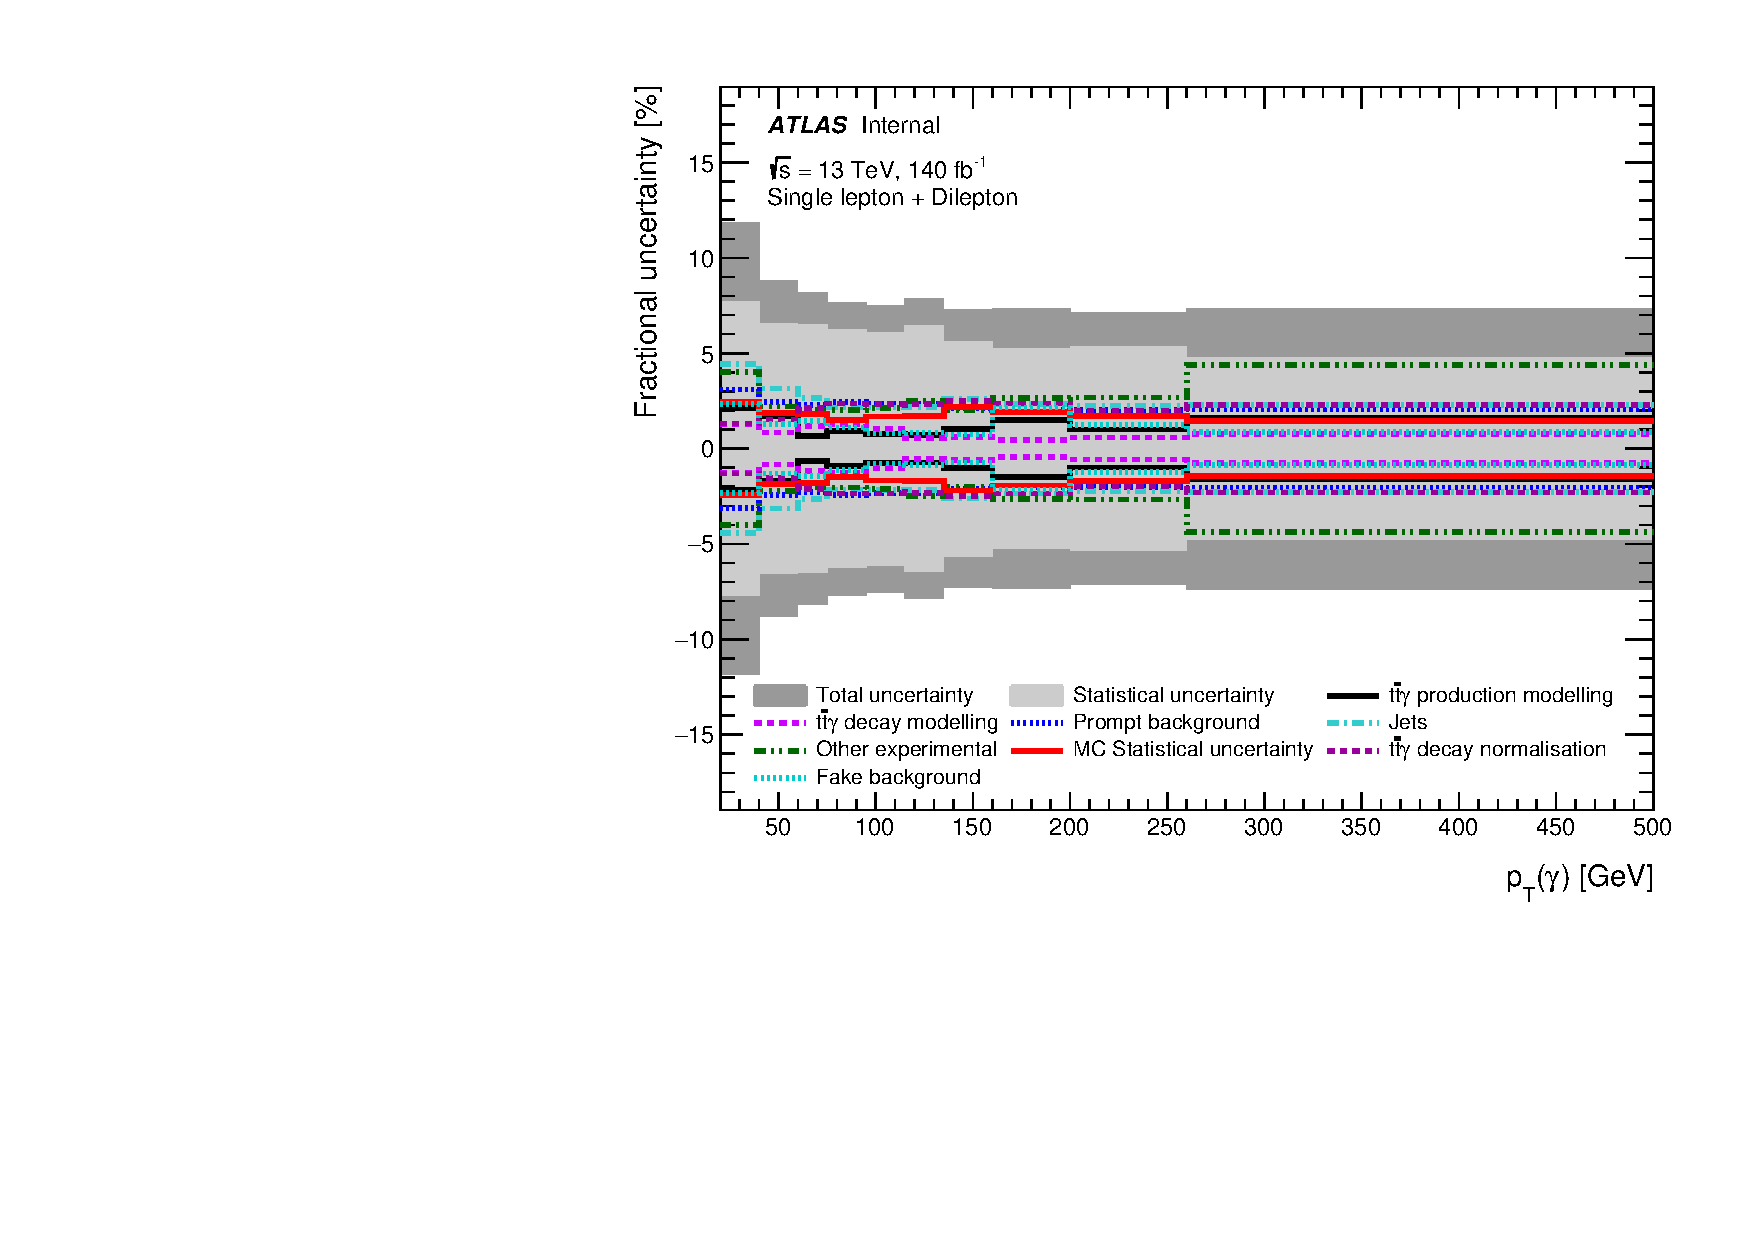
\includegraphics[width=0.80\textwidth]{figures/diff_xsec/groupedimpact-absolute-xsec/tty_prod_SLDL/GroupedImpact_tty_prod_pt_SLDL.pdf}\\
  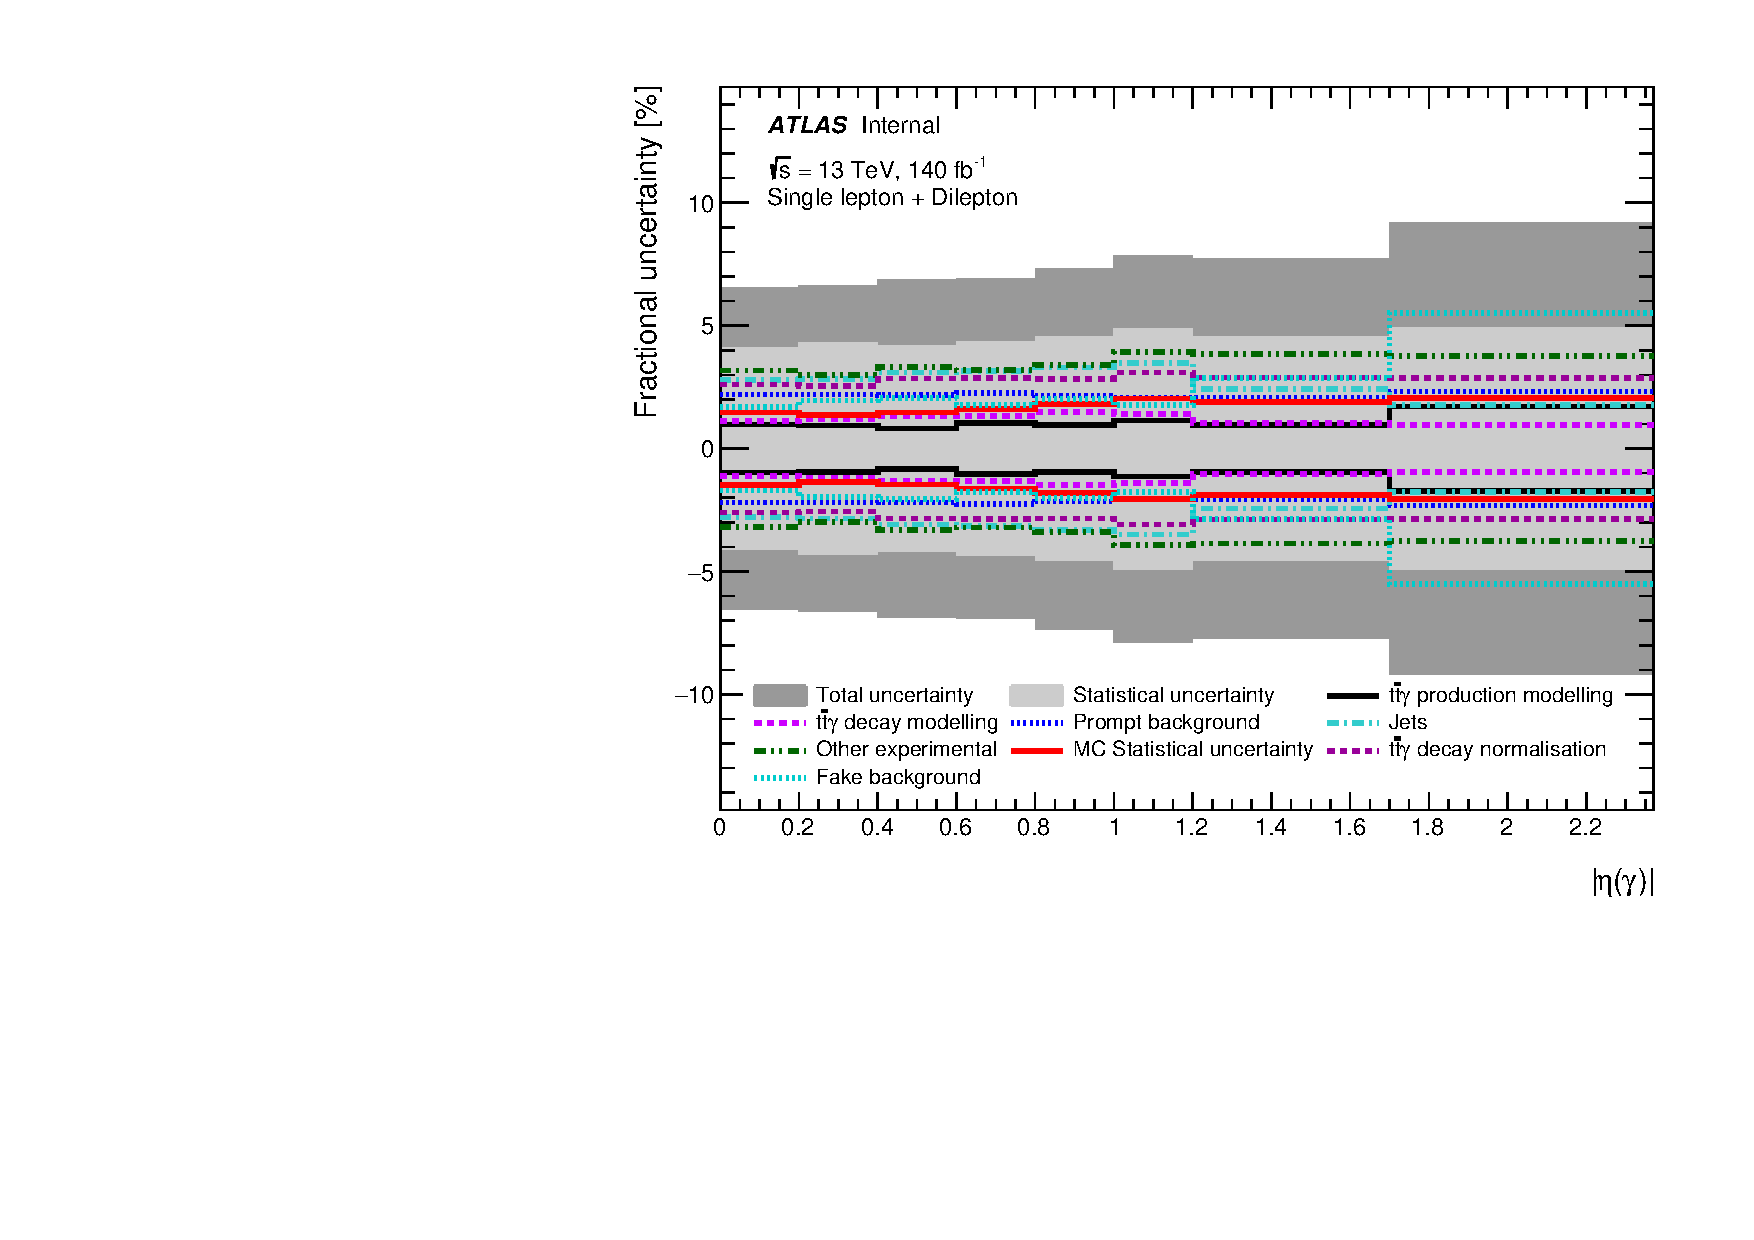
\includegraphics[width=0.80\textwidth]{figures/diff_xsec/groupedimpact-absolute-xsec/tty_prod_SLDL/GroupedImpact_tty_prod_eta_SLDL.pdf}%
\caption{The decomposed systematic uncertainties for absolute differential cross-sections as a function of the unfolded observables in combined single-lepton and dilepton channel for \tty production measurement.}
\label{fig:tty_prod_diff_SLDL_groupedimpact}
\end{figure}
\FloatBarrier

%%%%%%%%%%%%%%%%%%%%%%%%%%%%%%%%%% SLDL tty production normalized %%%%%%%%%%%%%%%%%%%%%%%%%%%%%%%%%%%%%%%%%%%%%
\begin{figure}[ht]
  \centering
  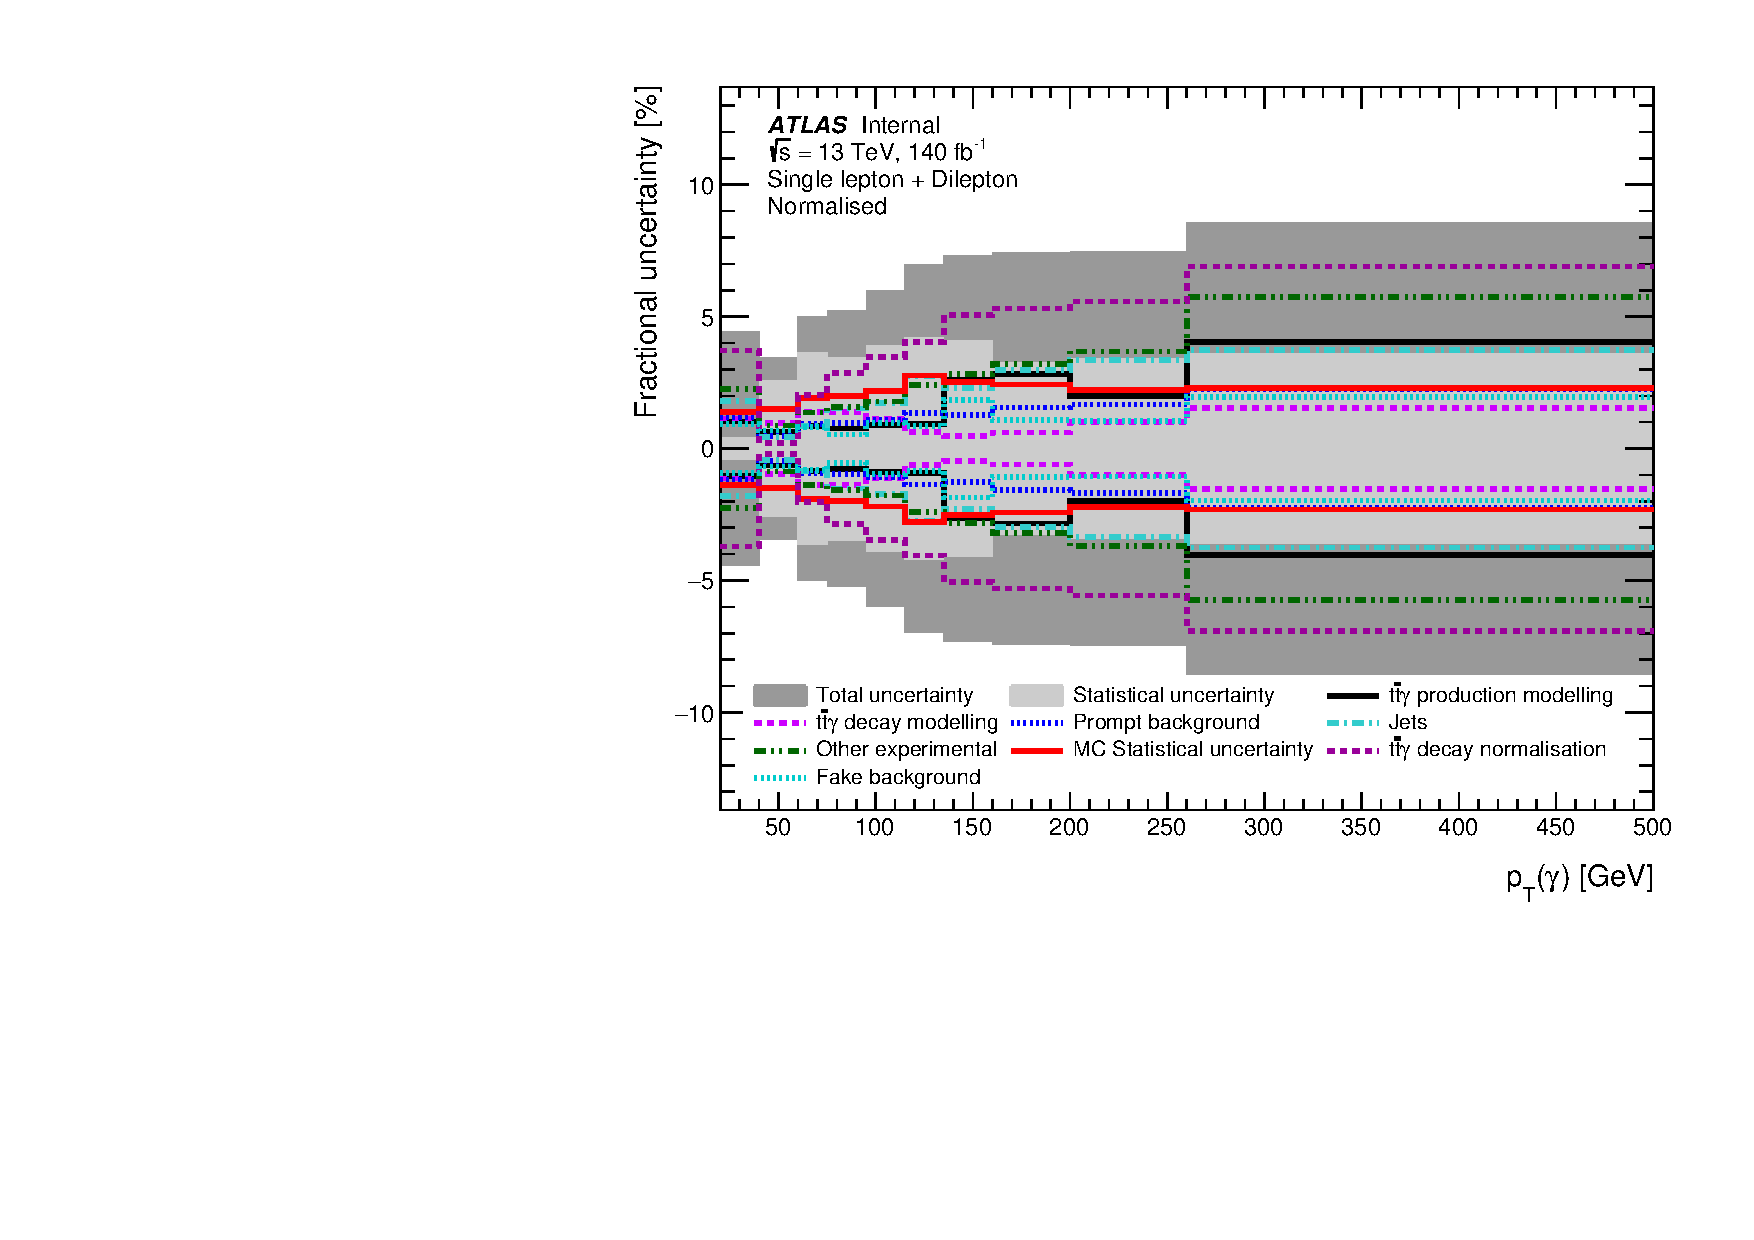
\includegraphics[width=0.80\textwidth]{figures/diff_xsec/groupedimpact-normalized-xsec/tty_prod_SLDL/GroupedImpact_tty_prod_pt_SLDL_norm.pdf}\\
  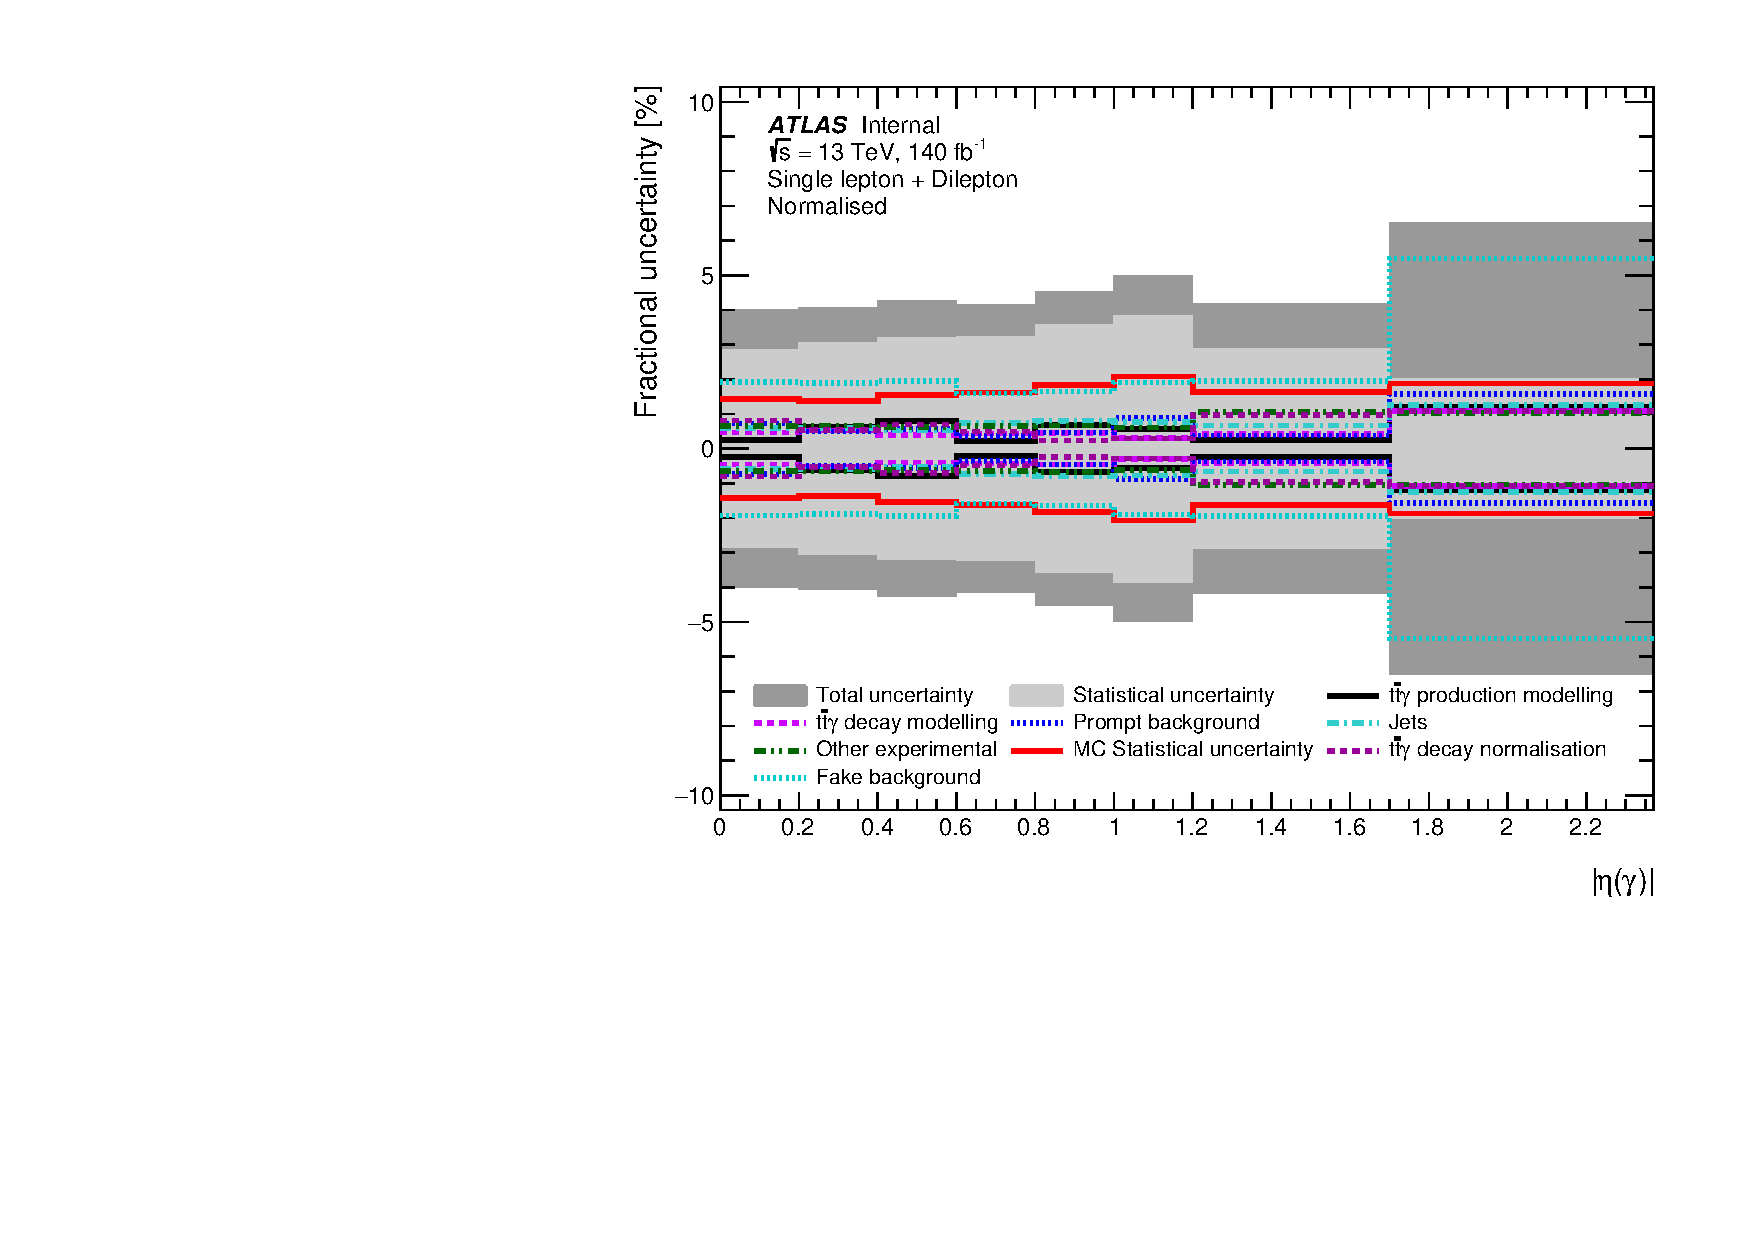
\includegraphics[width=0.80\textwidth]{figures/diff_xsec/groupedimpact-normalized-xsec/tty_prod_SLDL/GroupedImpact_tty_prod_eta_SLDL_norm.pdf}
\caption{The decomposed systematic uncertainties for normalized differential cross-sections as a function of the unfolded observables in combined single-lepton and dilepton channel for \tty production measurement.}
\label{fig:tty_prod_diff_SLDL_groupedimpact_normalized}
\end{figure}
\FloatBarrier


%%%%%%%%%%%%%%%%%%%%%%%%%%%%%%%%%% SL tty production %%%%%%%%%%%%%%%%%%%%%%%%%%%%%%%%%%%%%%%%%%%%%
\begin{figure}[ht]
  \centering
  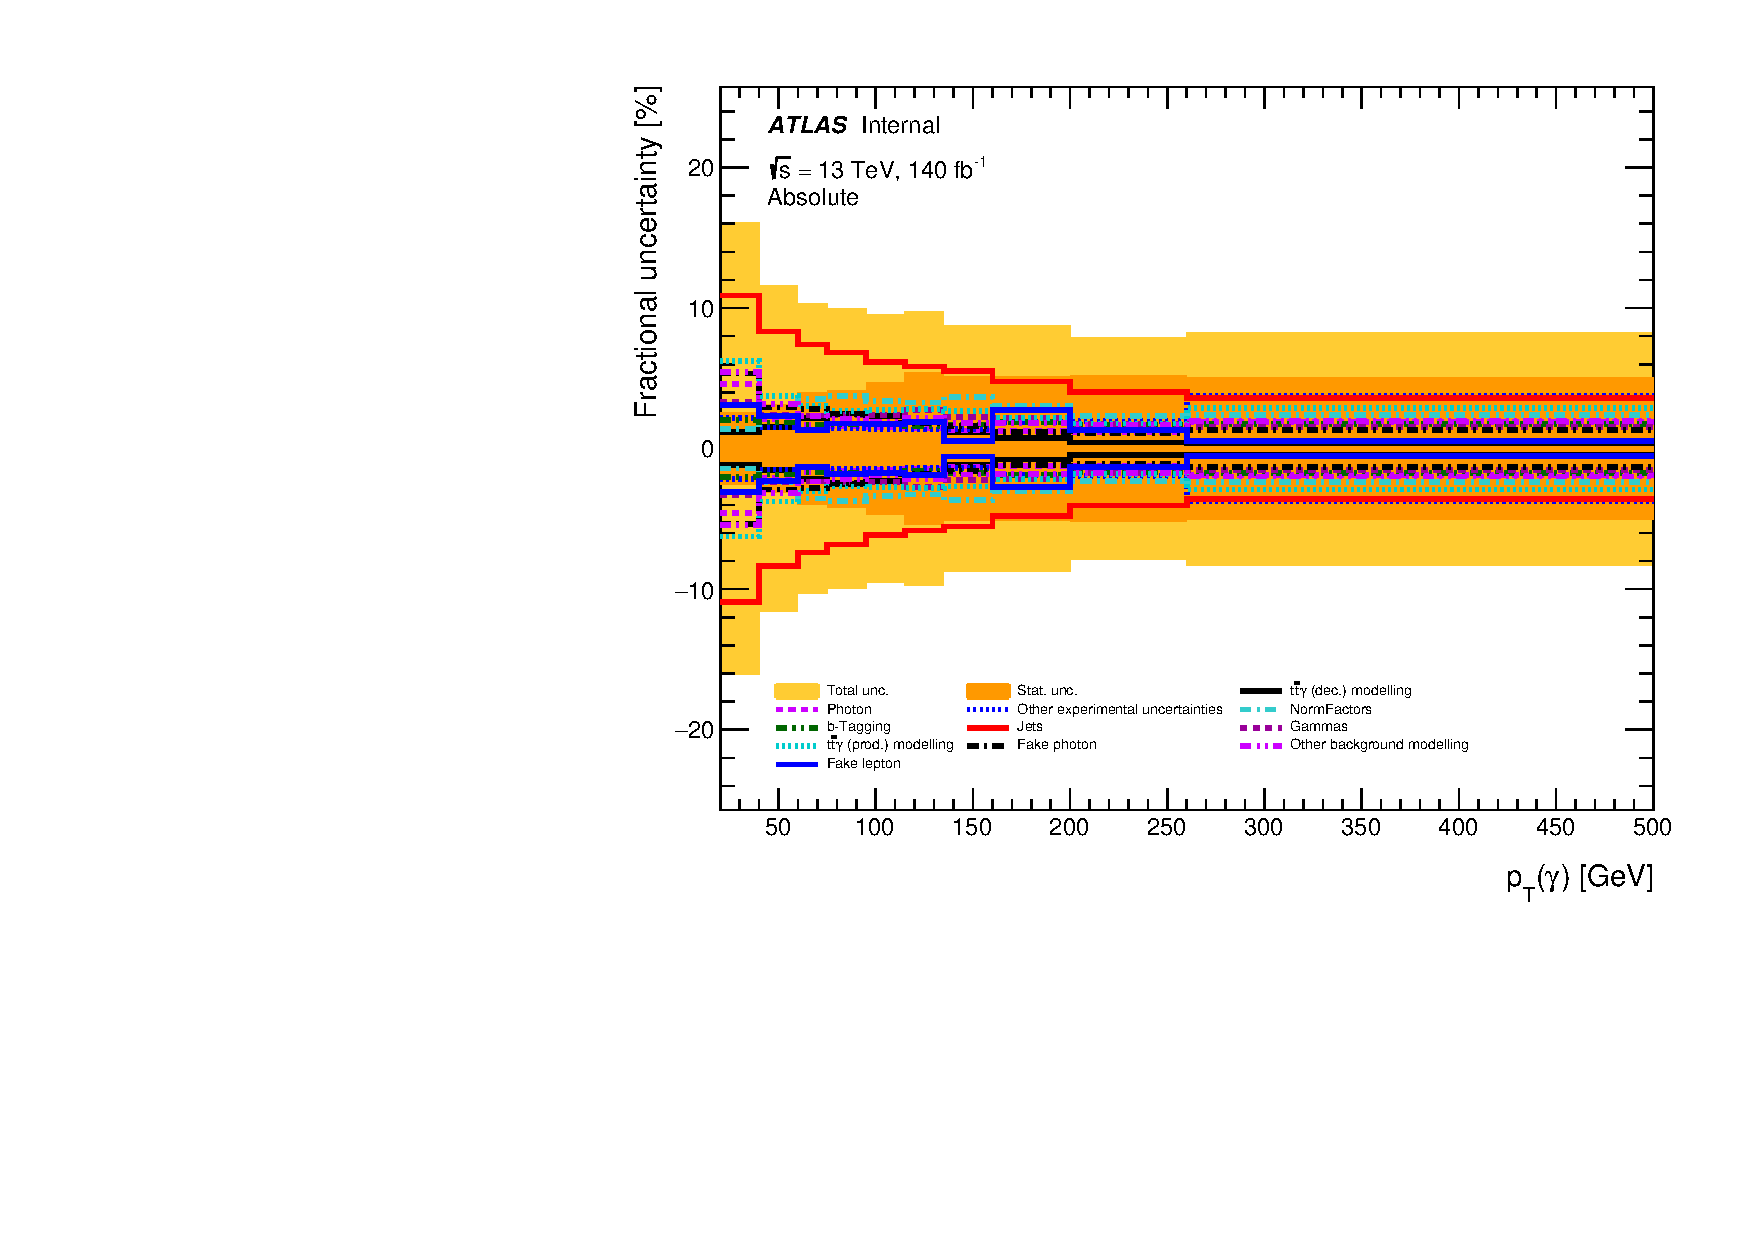
\includegraphics[width=0.45\textwidth]{figures/diff_xsec/groupedimpact-absolute-xsec/tty_prod_SL/Uncertainty_tty_pt.pdf}%
  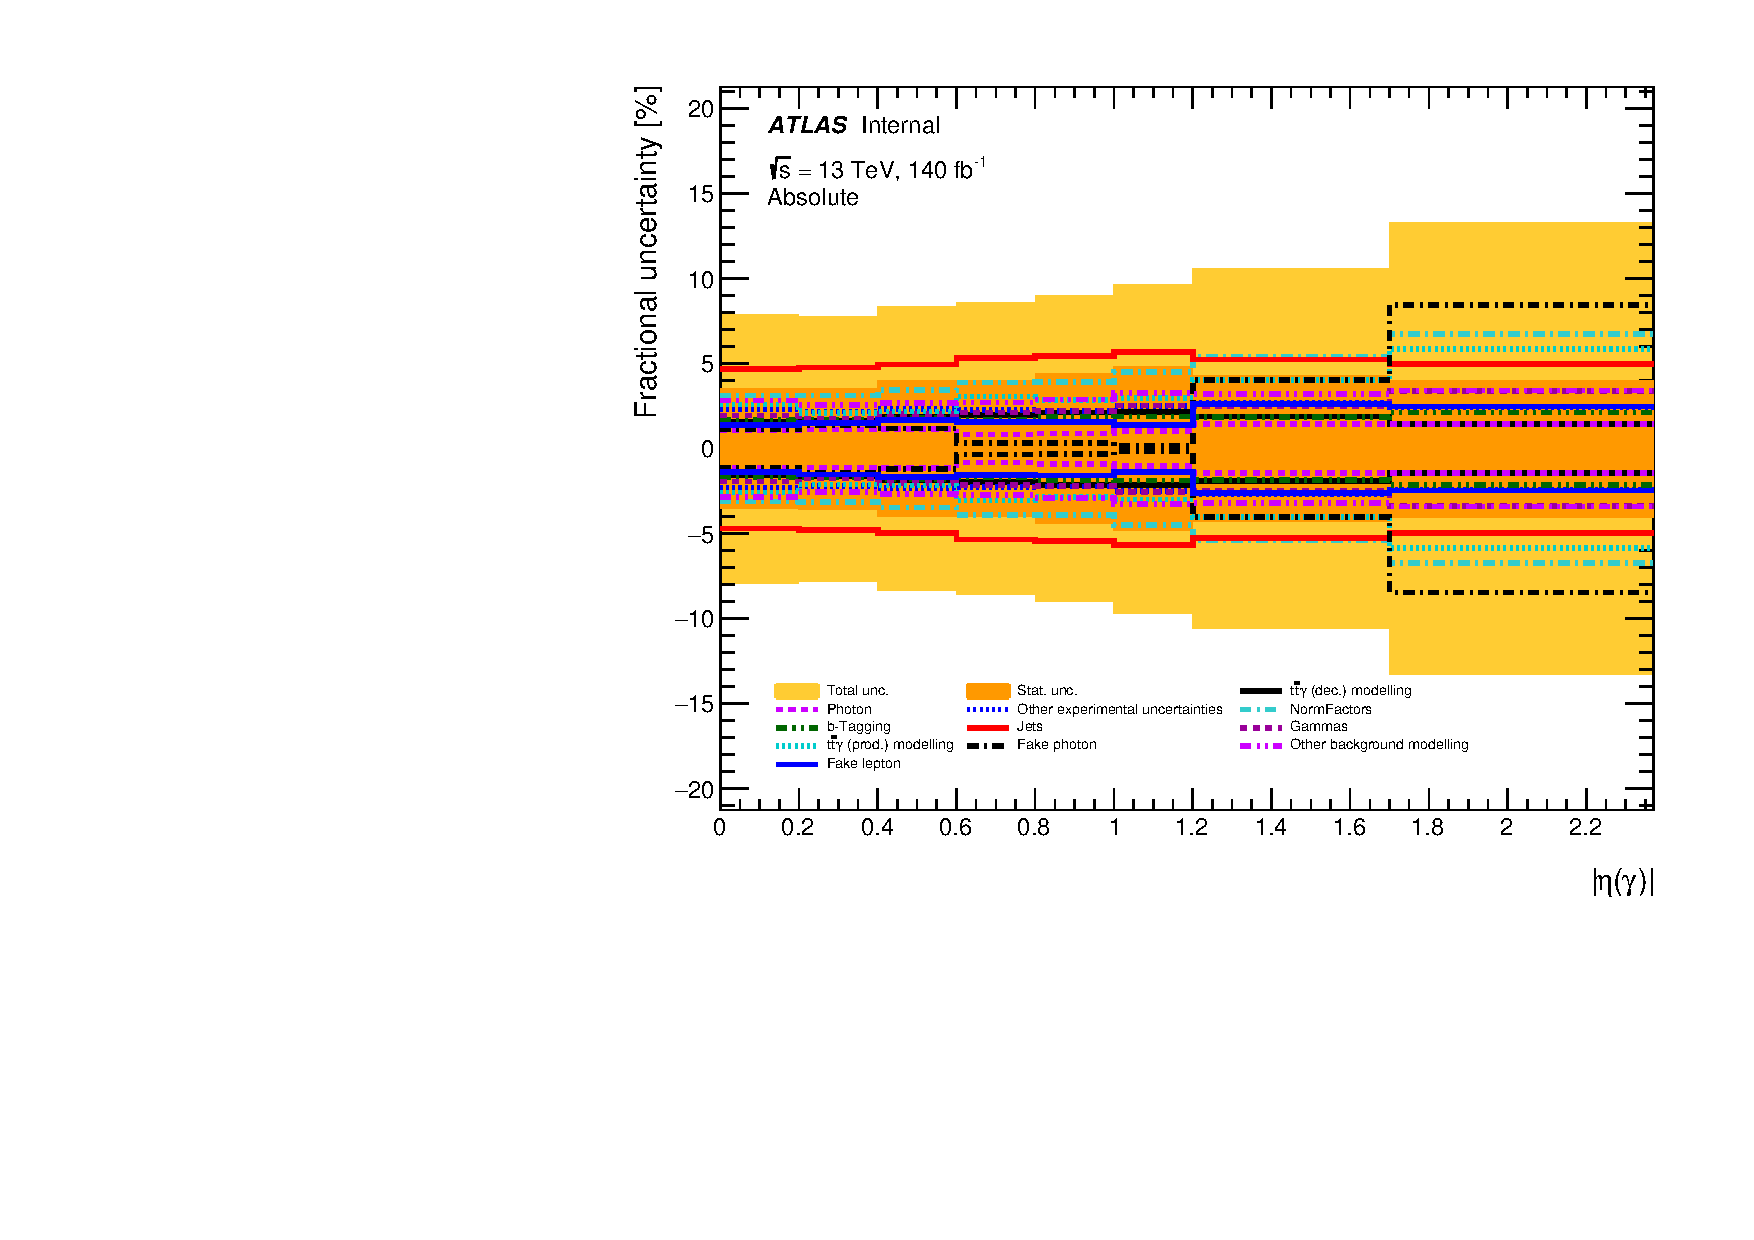
\includegraphics[width=0.45\textwidth]{figures/diff_xsec/groupedimpact-absolute-xsec/tty_prod_SL/Uncertainty_tty_eta.pdf}\\%
  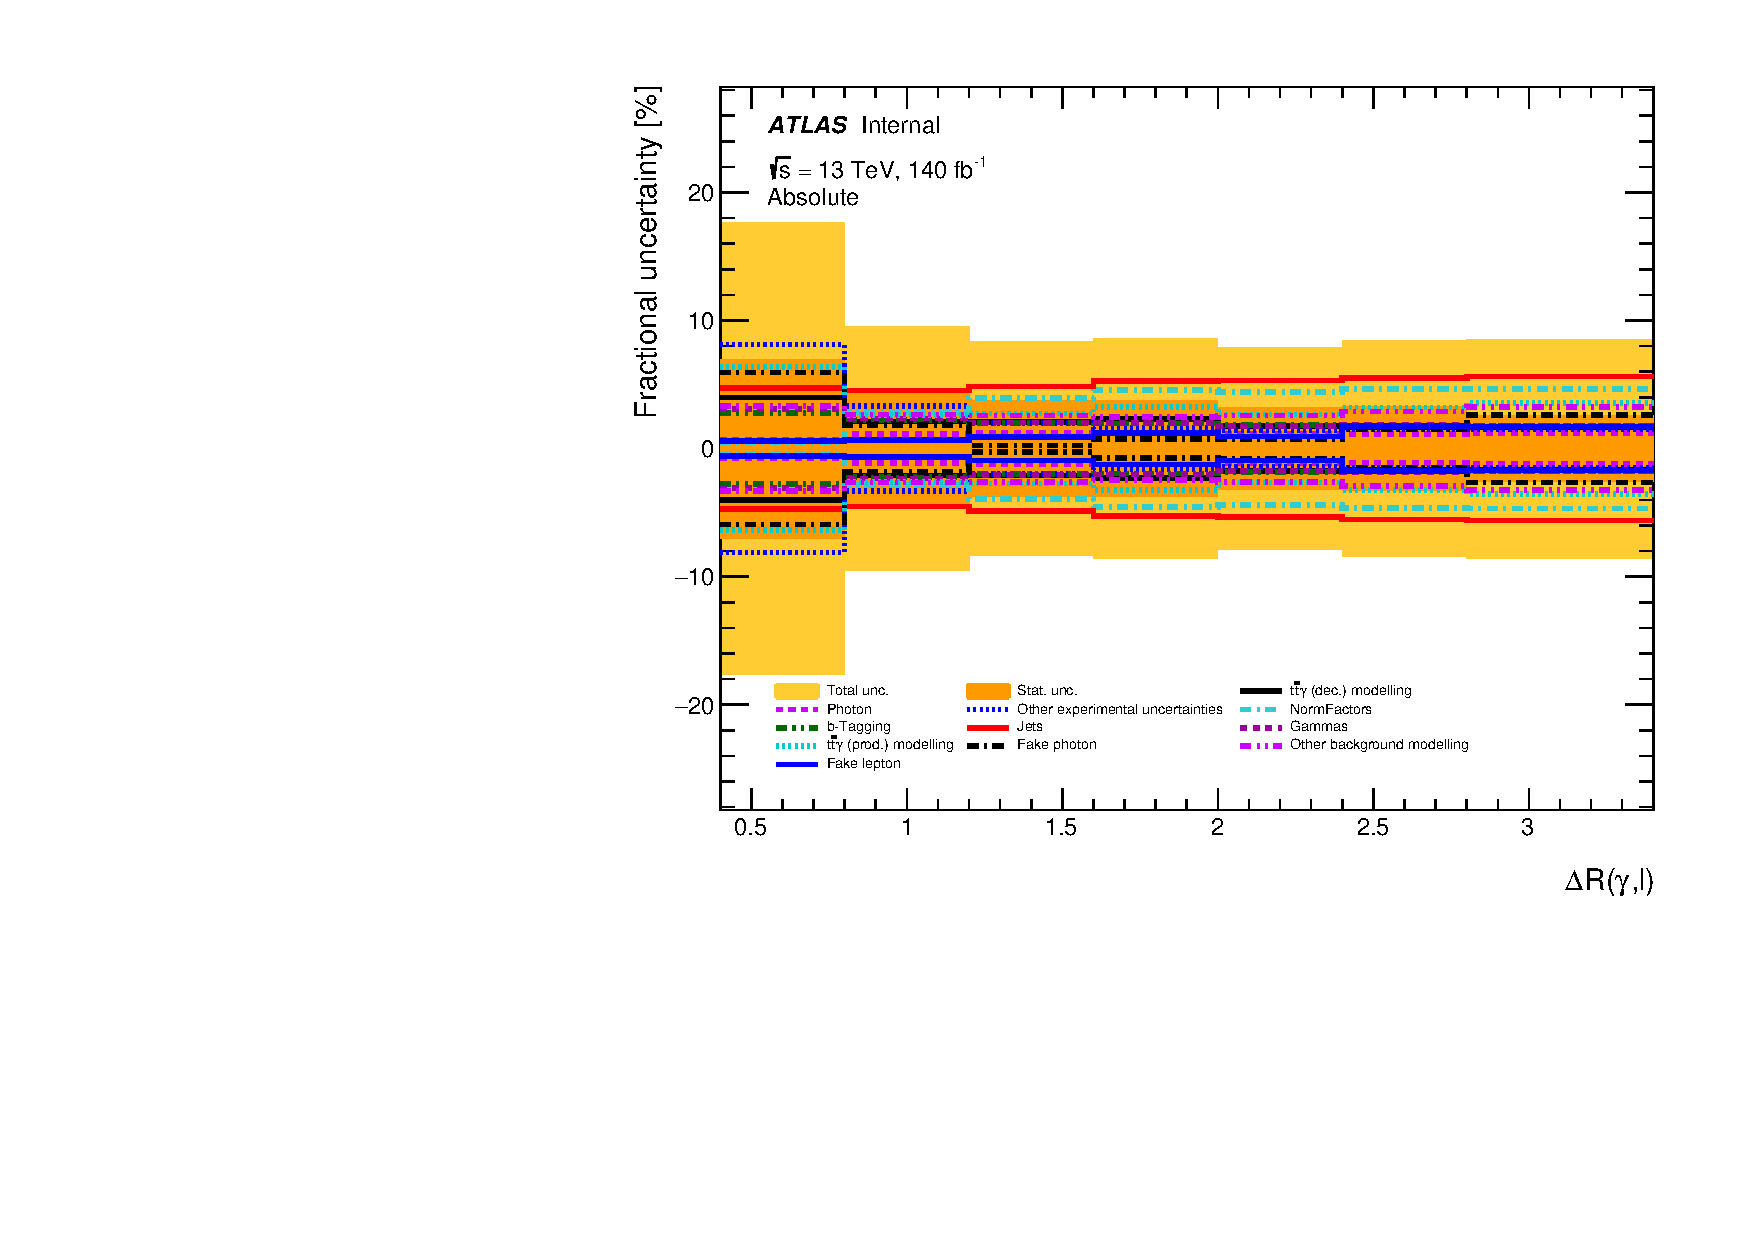
\includegraphics[width=0.45\textwidth]{figures/diff_xsec/groupedimpact-absolute-xsec/tty_prod_SL/Uncertainty_tty_drphl.pdf} %
  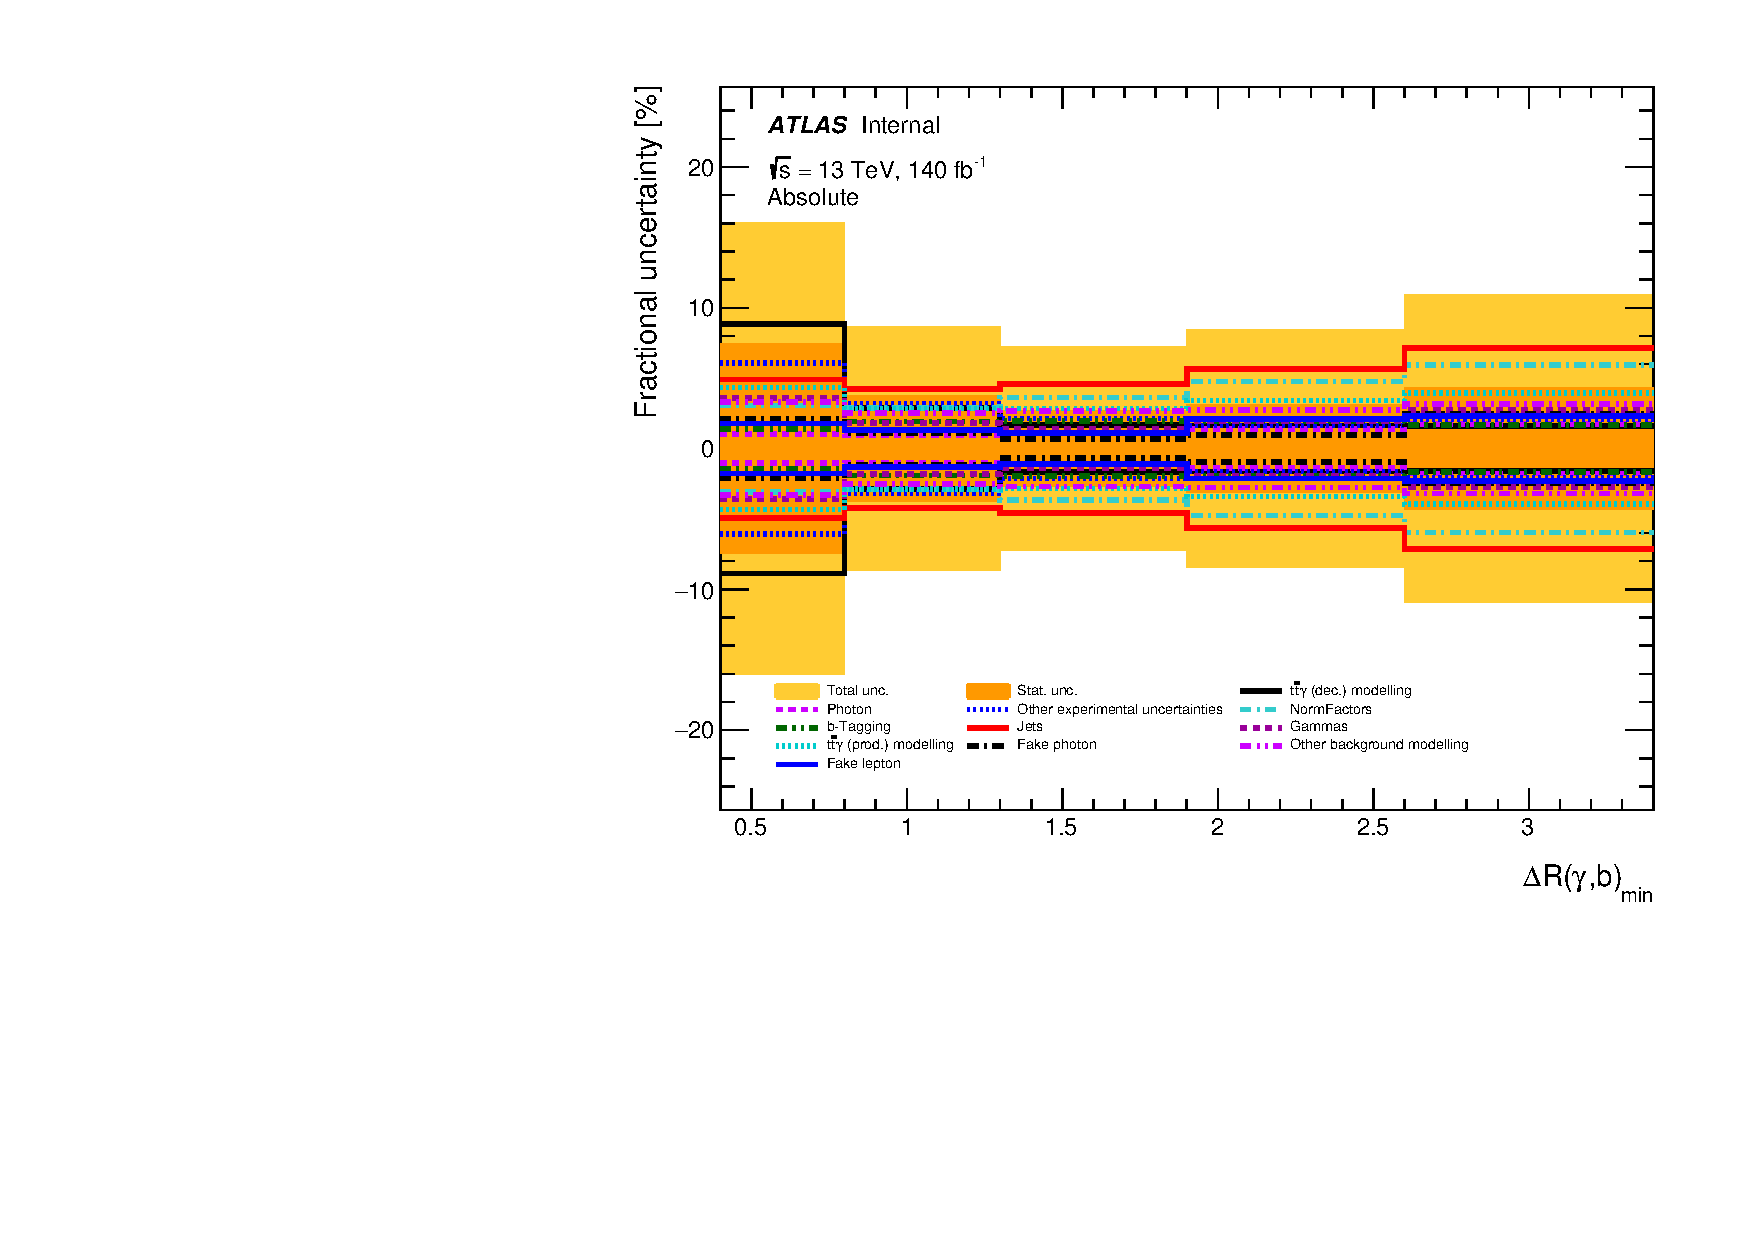
\includegraphics[width=0.45\textwidth]{figures/diff_xsec/groupedimpact-absolute-xsec/tty_prod_SL/Uncertainty_tty_drphb.pdf}\\%
  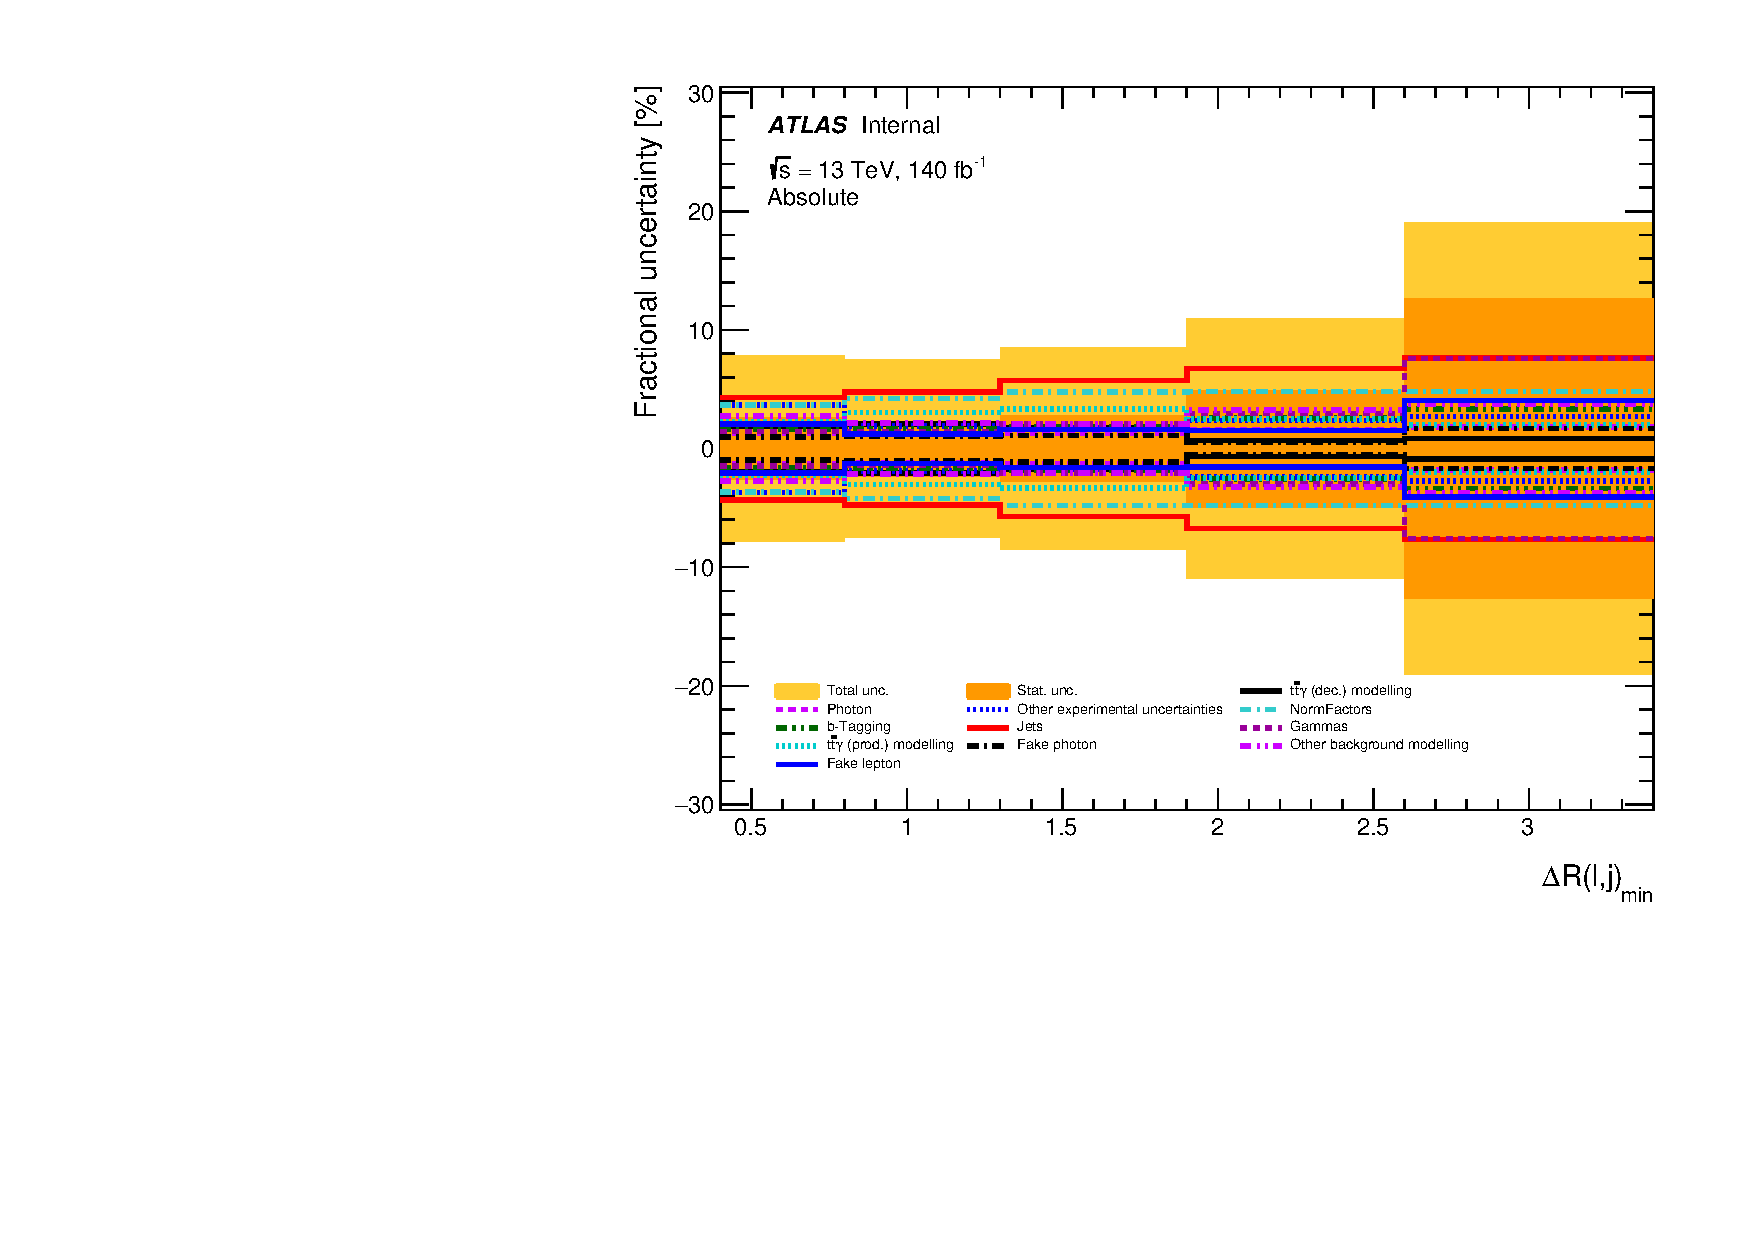
\includegraphics[width=0.45\textwidth]{figures/diff_xsec/groupedimpact-absolute-xsec/tty_prod_SL/Uncertainty_tty_drlj.pdf}% 
  \includegraphics[width=0.45\textwidth]{figures/diff_xsec/groupedimpact-absolute-xsec/tty_prod_SL/Uncertainty_tty_ptj1.pdf}\\%
\caption{The decomposed systematic uncertainties for absolute differential cross-sections as a function of the unfolded observables in single-lepton channel for \tty production measurement. 
(Note: the plots will be updated with same grouping as in Figure ~\ref{fig:tty_prod_diff_SLDL_groupedimpact}.)}
\label{fig:tty_prod_diff_Ljets_groupedimpact}
\end{figure}
\FloatBarrier

%%%%%%%%%%%%%%%%%%%%%%%%%%%%%%%%%% SL tty total %%%%%%%%%%%%%%%%%%%%%%%%%%%%%%%%%%%%%%%%%%%%%
\begin{figure}[ht]
  \centering
  \includegraphics[width=0.45\textwidth]{figures/diff_xsec/groupedimpact-absolute-xsec/tty_total_SL/Uncertainty_tty_pt.pdf}%
  \includegraphics[width=0.45\textwidth]{figures/diff_xsec/groupedimpact-absolute-xsec/tty_total_SL/Uncertainty_tty_eta.pdf}\\%
  \includegraphics[width=0.45\textwidth]{figures/diff_xsec/groupedimpact-absolute-xsec/tty_total_SL/Uncertainty_tty_drphl.pdf} %
  \includegraphics[width=0.45\textwidth]{figures/diff_xsec/groupedimpact-absolute-xsec/tty_total_SL/Uncertainty_tty_drphb.pdf}\\%
  \includegraphics[width=0.45\textwidth]{figures/diff_xsec/groupedimpact-absolute-xsec/tty_total_SL/Uncertainty_tty_drlj.pdf}% 
  \includegraphics[width=0.45\textwidth]{figures/diff_xsec/groupedimpact-absolute-xsec/tty_total_SL/Uncertainty_tty_ptj1.pdf}\\%
\caption{The decomposed systematic uncertainties for absolute differential cross-sections as a function of the unfolded observables in single-lepton channel for inclusive \tty measurement.
 (Note: the plots will be updated with same grouping as in Figure ~\ref{fig:tty_prod_diff_SLDL_groupedimpact}.)}
\label{fig:tty_total_diff_Ljets_groupedimpact}
\end{figure}
\FloatBarrier

%%%%%%%%%%%%%%%%%%%%%%%%%%%%%%%%%% DL tty production %%%%%%%%%%%%%%%%%%%%%%%%%%%%%%%%%%%%%%%%%%%%%
\begin{figure}[ht]
  \centering
  \includegraphics[width=0.45\textwidth]{figures/diff_xsec/groupedimpact-absolute-xsec//tty_prod_DL/Uncertainty_tty_pt.pdf}%
  \includegraphics[width=0.45\textwidth]{figures/diff_xsec/groupedimpact-absolute-xsec//tty_prod_DL/Uncertainty_tty_eta.pdf}\\%
  \includegraphics[width=0.45\textwidth]{figures/diff_xsec/groupedimpact-absolute-xsec//tty_prod_DL/Uncertainty_tty_min_drphl.pdf} %
  \includegraphics[width=0.45\textwidth]{figures/diff_xsec/groupedimpact-absolute-xsec//tty_prod_DL/Uncertainty_tty_drphb.pdf}\\%
  \includegraphics[width=0.45\textwidth]{figures/diff_xsec/groupedimpact-absolute-xsec//tty_prod_DL/Uncertainty_tty_drlj.pdf}% 
  \includegraphics[width=0.45\textwidth]{figures/diff_xsec/groupedimpact-absolute-xsec//tty_prod_DL/Uncertainty_tty_ptj1.pdf}\\%
\caption{The decomposed systematic uncertainties for absolute differential cross-sections as a function of the unfolded observables in dilepton channel for \tty production measurement.
 (Note: the plots will be updated with same grouping as in Figure ~\ref{fig:tty_prod_diff_SLDL_groupedimpact}.)}
\label{fig:tty_prod_diff_DL1_groupedimpact}
\end{figure}
\FloatBarrier

\begin{figure}[ht]
  \centering
  \includegraphics[width=0.45\textwidth]{figures/diff_xsec/groupedimpact-absolute-xsec/tty_prod_DL/Uncertainty_tty_drphl1.pdf}%
  \includegraphics[width=0.45\textwidth]{figures/diff_xsec/groupedimpact-absolute-xsec/tty_prod_DL/Uncertainty_tty_drphl2.pdf}\\%
  \includegraphics[width=0.45\textwidth]{figures/diff_xsec/groupedimpact-absolute-xsec/tty_prod_DL/Uncertainty_tty_ptll.pdf}%
  \includegraphics[width=0.45\textwidth]{figures/diff_xsec/groupedimpact-absolute-xsec/tty_prod_DL/Uncertainty_tty_dEtall.pdf}\\%
  \includegraphics[width=0.45\textwidth]{figures/diff_xsec/groupedimpact-absolute-xsec/tty_prod_DL/Uncertainty_tty_dPhill.pdf}% 
\caption{The decomposed systematic uncertainties for absolute differential cross-sections as a function of the unfolded observables in dilepton channel for \tty production measurement.
 (Note: the plots will be updated with same grouping as in Figure ~\ref{fig:tty_prod_diff_SLDL_groupedimpact}.)}
\label{fig:tty_prod_diff_DL2_groupedimpact}
\end{figure}
\FloatBarrier

%%%%%%%%%%%%%%%%%%%%%%%%%%%%%%%%%% DL tty total %%%%%%%%%%%%%%%%%%%%%%%%%%%%%%%%%%%%%%%%%%%%%
\begin{figure}[ht]
  \centering
  \includegraphics[width=0.45\textwidth]{figures/diff_xsec/groupedimpact-absolute-xsec/tty_total_DL/Uncertainty_tty2l_pt_all_syst.pdf}%
  \includegraphics[width=0.45\textwidth]{figures/diff_xsec/groupedimpact-absolute-xsec/tty_total_DL/Uncertainty_tty2l_eta_all_syst.pdf}\\%
  \includegraphics[width=0.45\textwidth]{figures/diff_xsec/groupedimpact-absolute-xsec/tty_total_DL/Uncertainty_tty2l_dr_all_syst.pdf}%
  \includegraphics[width=0.45\textwidth]{figures/diff_xsec/groupedimpact-absolute-xsec/tty_total_DL/Uncertainty_tty2l_drphb_all_syst.pdf}\\%
  \includegraphics[width=0.45\textwidth]{figures/diff_xsec/groupedimpact-absolute-xsec/tty_total_DL/Uncertainty_tty2l_drlj_all_syst.pdf}% 
  \includegraphics[width=0.45\textwidth]{figures/diff_xsec/groupedimpact-absolute-xsec/tty_total_DL/Uncertainty_tty2l_ptj1_all_syst.pdf}\\%
\caption{The decomposed systematic uncertainties for absolute differential cross-sections as a function of the unfolded observables in dilepton channel for inclusive \tty measurement.
 (Note: the plots will be updated with same grouping as in Figure ~\ref{fig:tty_prod_diff_SLDL_groupedimpact}.)}
\label{fig:tty_total_diff_DL1_groupedimpact}
\end{figure}
\FloatBarrier

\begin{figure}[ht]
  \centering
  \includegraphics[width=0.45\textwidth]{figures/diff_xsec/groupedimpact-absolute-xsec/tty_total_DL/Uncertainty_tty2l_dr1_all_syst.pdf}%
  \includegraphics[width=0.45\textwidth]{figures/diff_xsec/groupedimpact-absolute-xsec/tty_total_DL/Uncertainty_tty2l_dr2_all_syst.pdf}\\%
  \includegraphics[width=0.45\textwidth]{figures/diff_xsec/groupedimpact-absolute-xsec/tty_total_DL/Uncertainty_tty2l_dEtall_all_syst.pdf}%
  \includegraphics[width=0.45\textwidth]{figures/diff_xsec/groupedimpact-absolute-xsec/tty_total_DL/Uncertainty_tty2l_dPhill_all_syst.pdf}\\% 
\caption{The decomposed systematic uncertainties for absolute differential cross-sections as a function of the unfolded observables in dilepton channel for inclusive \tty measurement.
 (Note: the plots will be updated with same grouping as in Figure ~\ref{fig:tty_prod_diff_SLDL_groupedimpact}.)}
\label{fig:tty_total_diff_DL2_groupedimpact}
\end{figure}
\FloatBarrier


%%%%%%%%%%%%%%%%%%%%%%%%%%%%%%%%%%%%%%%%%%%%%%%%%%%%%%%%%%%%%%%%%%%%%%%%%%%%
%%%%%%%%%%%%%%%%%%%%%%% chi2 and p-values %%%%%%%%%%%%%%%%%%%%%%%%%%%%%%%%%%
%%%%%%%%%%%%%%%%%%%%%%%%%%%%%%%%%%%%%%%%%%%%%%%%%%%%%%%%%%%%%%%%%%%%%%%%%%%%


\begin{table}
  \scriptsize
  \centering
  \caption{$\chi^2$/ndf and $p$-values between the measured absolute and normalised cross-sections of \tty production and the NLO \MGNLO simulations interfaced with \PYTHIA[8] and \HERWIG[7].}
  \scalebox{0.9}{
  \begin{tabular}{l | c c | c c | c c |  c c }
  \toprule
    & \multicolumn{4}{c}{Absolute cross-sections} & \multicolumn{4}{c}{Normalised cross-sections} \\
    &  \multicolumn{2}{c}{MG5\_aMC@NLO+\Pythia[8]} & \multicolumn{2}{c}{MG5\_aMC@NLO+\Herwig[7]} &  \multicolumn{2}{c}{MG5\_aMC@NLO+\Pythia[8]} & \multicolumn{2}{c}{MG5\_aMC@NLO+\Herwig[7]}\\
  Variables & $\chi^2$/ndf & $p$-value & $\chi^2$/ndf & $p$-value & $\chi^2$/ndf & $p$-value & $\chi^2$/ndf & $p$-value \\
  \midrule
  \multicolumn{9}{c}{Single-lepton and dilepton combined} \\
  \midrule
  \pt($\gamma$) &	 10.1/10 &	 0.44 &	 9.0/10 &	 0.54 &	 15.0/9 &	 0.09 &	 10.4/9 & 	 0.32 \\			
  $|\eta|$($\gamma$) &	 14.6/8 &	 0.07 &	 13.5/8 &	 0.09 &	 10.4/7 &	 0.17 &	 10.5/7 & 	 0.16 \\	

  \bottomrule
  \end{tabular}
  \label{tab:chi2_ttyprod_sldl}
  }
  \end{table}
  \FloatBarrier





%%%%%%%%%%%%% tty total %%%%%%%%%%%%%%%%
  \begin{table}
    \scriptsize
    \centering
    \caption{$\chi^2$/ndf and $p$-values between the measured absolute and normalised cross-sections of the total \tty production and decay process and the LO $2\rightarrow 7$ \MGNLO simulation interfaced with \PYTHIA[8] and \HERWIG[7].}
    \scalebox{0.9}{
    \begin{tabular}{l | c c | c c | c c |  c c }
    \toprule
      & \multicolumn{4}{c}{Absolute cross-sections} & \multicolumn{4}{c}{Normalised cross-sections} \\
      &  \multicolumn{2}{c}{MG5\_aMC@NLO+\Pythia[8]} & \multicolumn{2}{c}{MG5\_aMC@NLO+\Herwig[7]} &  \multicolumn{2}{c}{MG5\_aMC@NLO+\Pythia[8]} & \multicolumn{2}{c}{MG5\_aMC@NLO+\Herwig[7]}\\
    Variables & $\chi^2$/ndf & $p$-value & $\chi^2$/ndf & $p$-value & $\chi^2$/ndf & $p$-value & $\chi^2$/ndf & $p$-value \\
    \midrule
    \multicolumn{9}{c}{Single-lepton channel} \\
    \midrule
    \pt($\gamma$) &	 12.9/10&	 0.23&	 8.7/10&	 0.56&	 122.4/9&	 $<0.01$ &	 31.6/9& 	 $<0.01$ \\ 
                    
    $|\eta|$($\gamma$)	& 13.3/8&	 0.1&	 13.3/8&	 0.1&	 12.2/7&	 0.09&	 13.1/7& 	 0.07 \\
                    
    $\Delta R(\gamma, \ell)$ &	 15.2/7&	 0.03&	 14.2/7&	 0.05&	 18.5/6&	 0.01&	 17.3/6& 	 0.01 \\
                    
    $\Delta R(\gamma, b)_{min}$ &	 8.6/5&	 0.12&	 5.9/5&	 0.31&	 9.1/4&	 0.06&	 5.8/4& 	 0.21 \\
                    
    $\Delta R(\ell, j)_{min}$	& 4.7/5&	 0.46&	 2.9/5&	 0.71&	 0.8/4&	 0.93&	 0.9/4& 	 0.93 \\
                    
    $\pt(j_1)$	& 25.2/5&	 $<0.01$ &	 43.5/5&	 $<0.01$ &	 27.8/4&	 $<0.01$ &	 45.2/4& 	 $<0.01$  \\
    \midrule
    \multicolumn{9}{c}{Dilepton channel} \\
    \midrule
    \pt($\gamma$) &	 7.5/6&	 0.28&	 4.3/6&	 0.64&	 6.4/5&	 0.27&	 4.1/5& 	 0.53 \\
                    
    $|\eta|$($\gamma$)	& 5.3/8&	 0.73&	 6.5/8&	 0.59&	 5.5/7&	 0.6&	 6.8/7& 	 0.45 \\
                    
    $\Delta R(\gamma, \ell)_{min}$ &	 24.7/7&	 $<0.01$ &	 24.3/7&	 $<0.01$ &	 21.0/6&	 $<0.01$ &	 20.7/6& 	 $<0.01$  \\
                    
    $\Delta R(\gamma, \ell_1)$ &      	 9.1/7&	 0.25&	 7.7/7&	 0.36&	 9.0/6&	 0.17&	 7.5/6& 	 0.28 \\
                    
    $\Delta R(\gamma, \ell_2)$ &      	 17.1/7&	 0.02&	 18.1/7&	 0.01&	 16.7/6&	 0.01&	 17.7/6& 	 0.01 \\
                    
    \Detall &	 4.0/7&	 0.78&	 7.0/7&	 0.43&	 3.3/6&	 0.78&	 5.8/6& 	 0.45 \\
                    
    \Dphill &	 35.8/8&	 $<0.01$ &	 37.6/8&	 $<0.01$ &	 35.6/7&	 $<0.01$ &	 37.3/7& 	 $<0.01$  \\
                    
    $\pt(\ell,\ell)$	& 6.5/6&	 0.37&	 12.5/6&	 0.05&	 5.8/5&	 0.33&	 11.5/5& 	 0.04 \\
                    
    $\Delta R(\gamma, b)_{min}$ &	 0.7/5&	 0.98&	 2.4/5&	 0.79&	 0.7/4&	 0.95&	 2.4/4& 	 0.66 \\
                    
    $\Delta R(\ell, j)_{min}$	& 6.1/5&	 0.3&	 8.9/5&	 0.11&	 9.9/4&	 0.04&	 12.4/4& 	 0.01 \\
                    
    $\pt(j_1)$	& 11.5/5&	 0.04&	 21.1/5&	 $<0.01$ &	 10.4/4&	 0.03&	 19.3/4& 	 $<0.01$  \\
    \bottomrule
    \end{tabular}
    \label{tab:chi2_tty}
    }
    \end{table}
    
  \FloatBarrier

